\documentclass[12pt]{article}

%----------------------------------------
% PACKAGES
%----------------------------------------
\usepackage[margin=1in]{geometry}    % Set margins
\usepackage{graphicx}               % For figures
\usepackage{epstopdf}               % For EPS figure inclusion
\usepackage{amsmath,amssymb}        % For math
\usepackage{enumerate}              % For enumeration styles
\usepackage[numbers,sort&compress]{natbib}  % For references
\usepackage{lmodern}                % Enhanced Latin Modern font
\usepackage{booktabs}               % For better tables
\usepackage{subcaption}             % For sub-figures
\usepackage{hyperref}               % For hyperlinks
\usepackage{xcolor}                 % For color usage
\usepackage{setspace}               % For line spacing
\usepackage{authblk}                % For author and affiliation
\usepackage{caption}

%----------------------------------------
% HYPERREF CONFIGURATION
%----------------------------------------
\hypersetup{
    colorlinks=true,
    linkcolor=blue,
    citecolor=blue,
    urlcolor=blue
}

%----------------------------------------
% TITLE AND AUTHOR INFO
%----------------------------------------
\title{Machine Learning-Based Sentiment Analysis
of Financial Texts}

\author[1]{Chuan Jia(No. 17), Bo li(No. 9), Sheng Su(No. 10)\footnote{The authors are listed in surname order. All authors contributed equally to this work.}}

\date{}  % If no date is required, keep it blank

%----------------------------------------
% DOCUMENT START
%----------------------------------------
\begin{document}
\maketitle

%----------------------------------------
% ABSTRACT
%----------------------------------------
\begin{abstract}
With the widespread adoption of the Internet, cloud computing, and big data, significant transformations have occurred in financial information processing. A vast amount of financial texts, such as news, reports, and social media content, have become crucial resources for formulating investment strategies, asset evaluation, and market forecasting. These texts not only contain numerical data and facts but also embody emotional signals that influence investment decisions. Integrating emotional signals into analytical frameworks helps enhance the rationality and predictability of investment strategies. However, the scarcity of Chinese financial sentiment corpora limits the application of deep learning and pre-trained models (such as BERT) in Chinese sentiment analysis. To address this, we propose a data-driven approach that first utilizes a Transformer-based neural machine translation model to convert English financial sentiment corpora into Chinese, then employs a Chinese sentiment lexicon for annotation, and finally fine-tunes the BERT model to improve Chinese sentiment classification performance. Nevertheless, the emergence of "meaningless Chinese words" during the translation process indicates deficiencies in the model's mapping of specialized terminology. We also explore the possibility of replacing or supplementing BERT with Bayesian or traditional machine learning methods, which sometimes offer advantages in terms of accuracy and interpretability.

\textbf{Keywords}: financial text information, sentiment analysis, Transformer model, BERT model, data augmentation, machine translation, Bayesian interpretability
\end{abstract}

\setstretch{1.2}  % Adjust line spacing if desired

%----------------------------------------
% 1. INTRODUCTION
%----------------------------------------
\section{Introduction}
\label{sec:intro}

Financial activities lie at the heart of modern economic systems, shaping everything from micro-level investment decisions to macro-level policies. Driven by developments in the Internet and data analytics, enormous quantities of financial text---including news, reports, and social media commentary---are now readily available. While traditional analyses often rely on explicit indicators like pricing data or fundamental ratios, they may omit subtle emotional signals embedded within these texts.

Latent sentiments, such as fear, optimism, or skepticism, can influence market trends by affecting trading decisions and shaping public opinion. For instance, a speculative rumor shared on social media regarding a potential product failure might trigger massive sell-offs, contributing to short-term volatility. More comprehensive decision-making frameworks must, therefore, incorporate these emotional cues.

Despite the abundance of English-language financial sentiment corpora, labeled Chinese financial datasets remain scarce. This gap has motivated us to translate high-quality English content into Chinese, thus enlarging our corpus and addressing data insufficiency for a specialized domain. However, translation alone is not a complete solution---certain terms do not map neatly between languages, especially when dealing with finance-specific jargon. Additionally, advanced solutions (such as graph-based methods for unified semantic representation) may be needed to further mitigate mismatches introduced by translation.

This study offers three primary contributions:

\begin{enumerate}
    \item \textbf{Data Augmentation via Translation:} We employ a Transformer-based NMT model to convert English financial sentiment texts into Chinese, expanding the availability of labeled data for model training.
    \item \textbf{Lexicon-Based Annotation:} By leveraging a domain-specific Chinese financial sentiment lexicon, we automatically assign polarity labels to large volumes of text, enriching the dataset further.
    \item \textbf{BERT Fine-Tuning and Alternatives:} We fine-tune a pre-trained BERT model for Chinese financial sentiment classification. Additionally, we consider how Bayesian or traditional machine learning methods may sometimes outperform or offer clearer interpretability compared to deep neural networks in certain contexts.
\end{enumerate}

%----------------------------------------
% 2. RELATED WORK
%----------------------------------------
\section{Related Work}
\label{sec:relatedwork}

\subsection{Financial Sentiment Analysis}
Financial sentiment analysis aims to quantify subjective feelings or attitudes from unstructured text. Studies have shown that managerial tone, media coverage, and user-generated content can all be predictive of stock returns and market volatility \cite{ref3,ref4}. Despite substantial progress in English financial text analysis, limited research has focused on Chinese corpora, due primarily to the shortage of annotated data and the linguistic complexity of Chinese.

\subsection{Transformer Models in NLP}
The Transformer architecture proposed by Vaswani et al. \cite{ref1} uses multi-head self-attention to capture global dependencies in text. This architecture has proven adept at machine translation, sentiment analysis, and question answering. In recent years, various Transformer-based models (e.g., BERT, GPT variants) have achieved state-of-the-art results across numerous NLP benchmarks. Figure \ref{fig:attention_mechanisms} illustrates the core components of Transformer models.

\begin{figure}[!ht]
	\centering
	\begin{subfigure}[b]{0.32\textwidth}
		\centering
		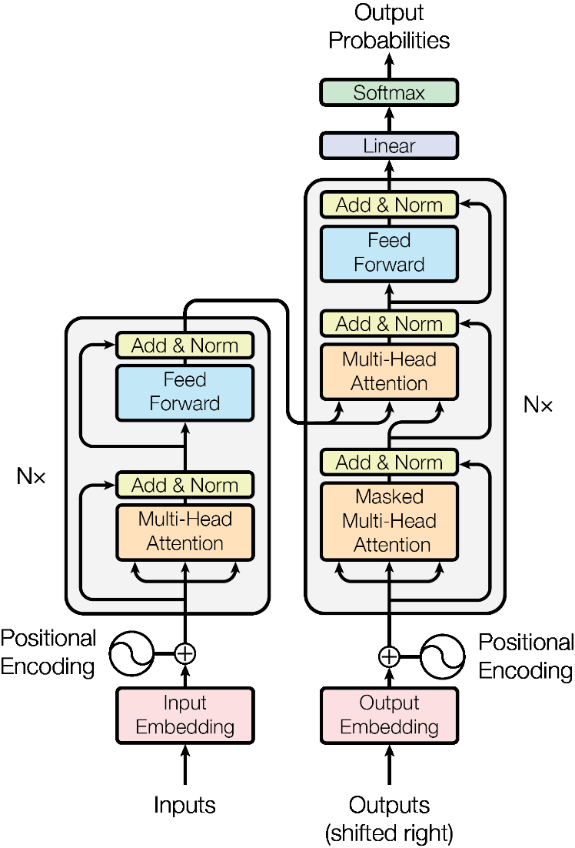
\includegraphics[height=4cm]{attention.png}
		\caption{Attention mechanism.}
	\end{subfigure}
	\hfill
	\begin{subfigure}[b]{0.32\textwidth}
		\centering
		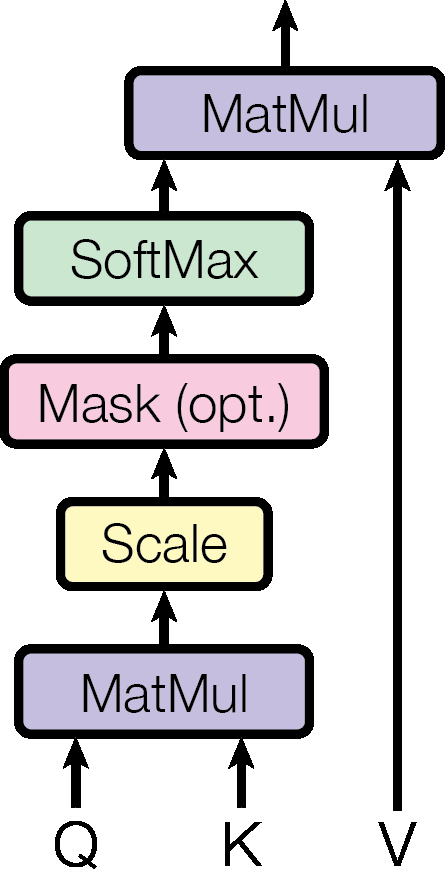
\includegraphics[height=4cm]{self_attention_mechanism.png}
		\caption{Self-attention}
	\end{subfigure}
	\hfill
	\begin{subfigure}[b]{0.32\textwidth}
		\centering
		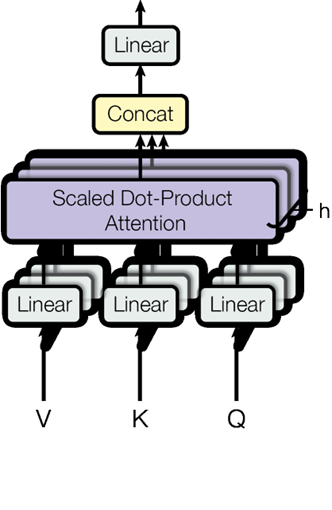
\includegraphics[height=4cm]{multihead_attention.png}
		\caption{Multi-head attention}
	\end{subfigure}
	\caption{Illustrations of attention mechanisms in Transformer models.}
	\label{fig:attention_mechanisms}
\end{figure}

\subsection{BERT and Domain Adaptation}
BERT \cite{ref2} uses a bidirectional encoder to learn contextual representations through masked language modeling and next sentence prediction. Fine-tuning BERT on domain-specific corpora often yields significant performance improvements. In financial domains, specialized BERT variants or further pre-training on finance-related text can better capture terminology and context.

\begin{figure}[!ht]
	\centering
	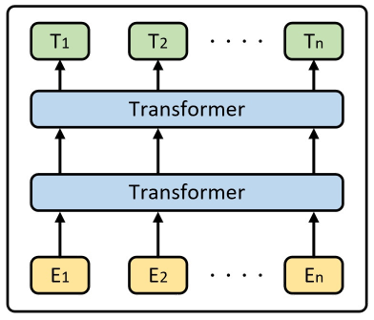
\includegraphics[height=4cm]{BERT.png}
	\caption{BERT architecture.}
\end{figure}

%----------------------------------------
% 3. METHODOLOGY
%----------------------------------------
\section{Methodology}

\subsection{Data Collection and Preprocessing}
We gathered 54,749 Chinese financial news articles from various reputable sources, including 40,000 Chinese financial news articles and 14,749 translated English financial texts. The latter were translated using a Transformer-based NMT model. We also utilized a Chinese financial sentiment lexicon to pre-label a subset of unannotated texts, enriching the training set. Each news is labeled with a sentiment category: \textbf{positive}, \textbf{neutral}, or \textbf{negative}. 

All data were tokenized using a Chinese tokenizer (\textit{jieba}). For the unannotated subset, we employed a Chinese financial sentiment lexicon to pre-label texts. This procedure facilitated the creation of an enriched training set that better captures domain-specific language features.

\paragraph{Data Statistics and Visualization}
We conducted exploratory data analysis to understand the distribution of sentiment categories, text lengths, and word frequencies. Figures \ref{fig:wordclouds}--\ref{fig:sentiment_distribution} illustrate the word clouds, top words, text length distributions, and sentiment category distributions in our dataset.

\begin{figure}[!ht]
	\centering
	\begin{subfigure}[b]{0.32\textwidth}
		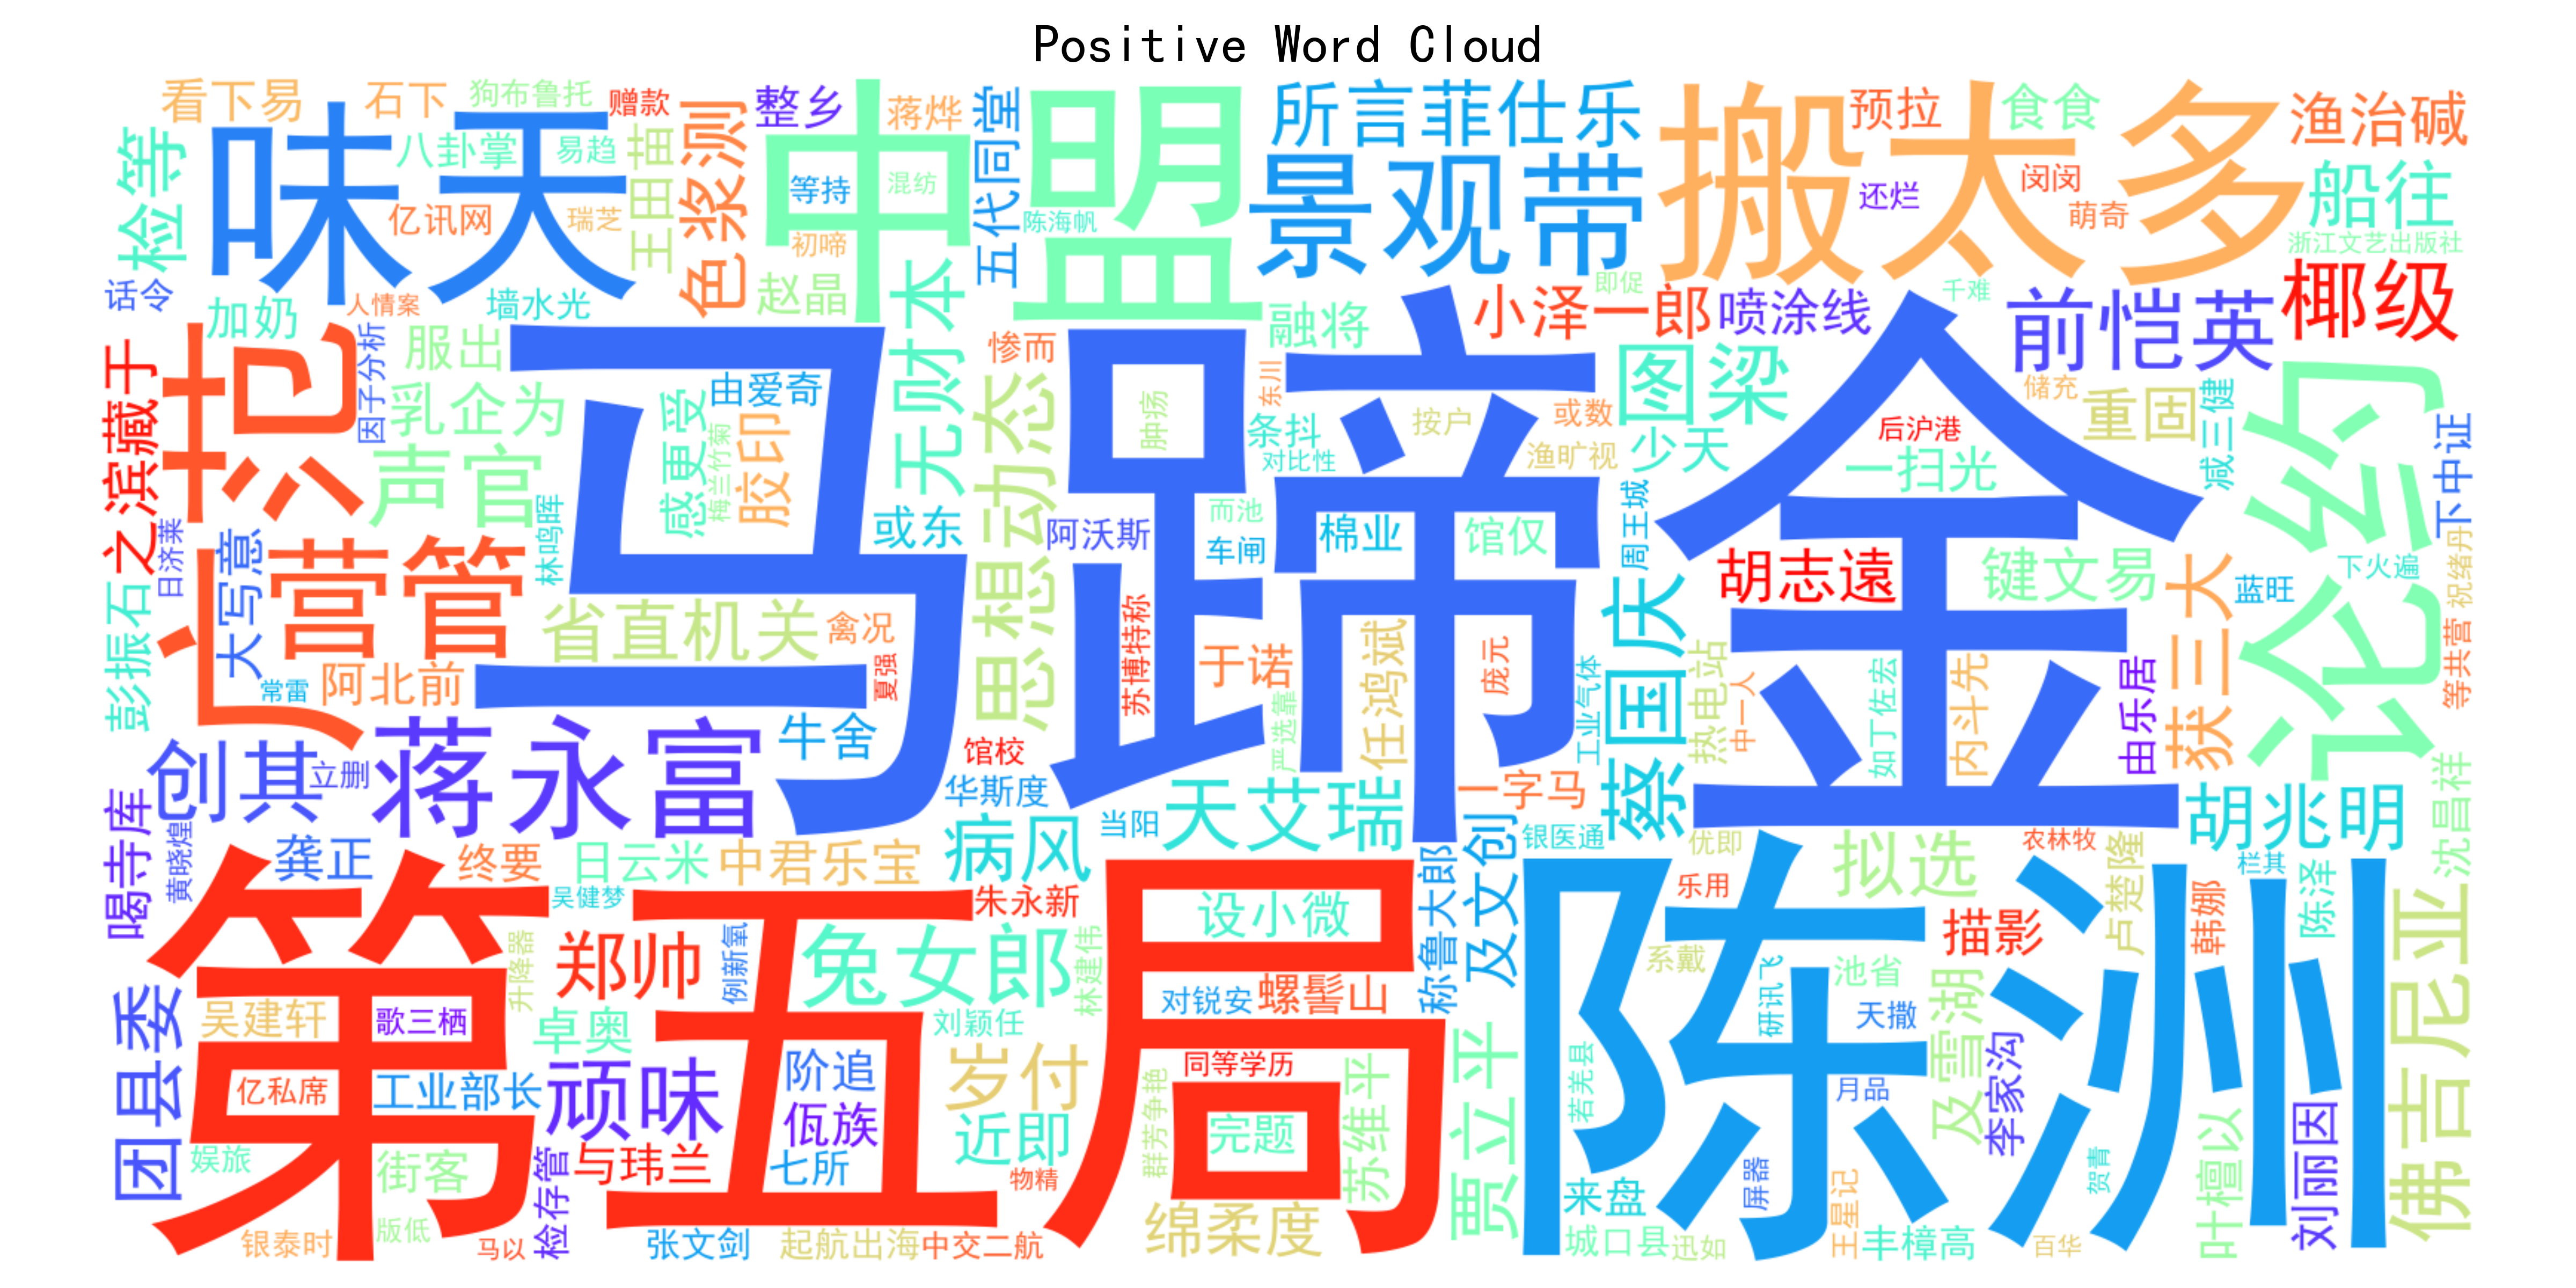
\includegraphics[width=\linewidth]{wordcloud_positive.png}
		\caption{Word cloud of positive}
	\end{subfigure}
	\hfill
	\begin{subfigure}[b]{0.32\textwidth}
		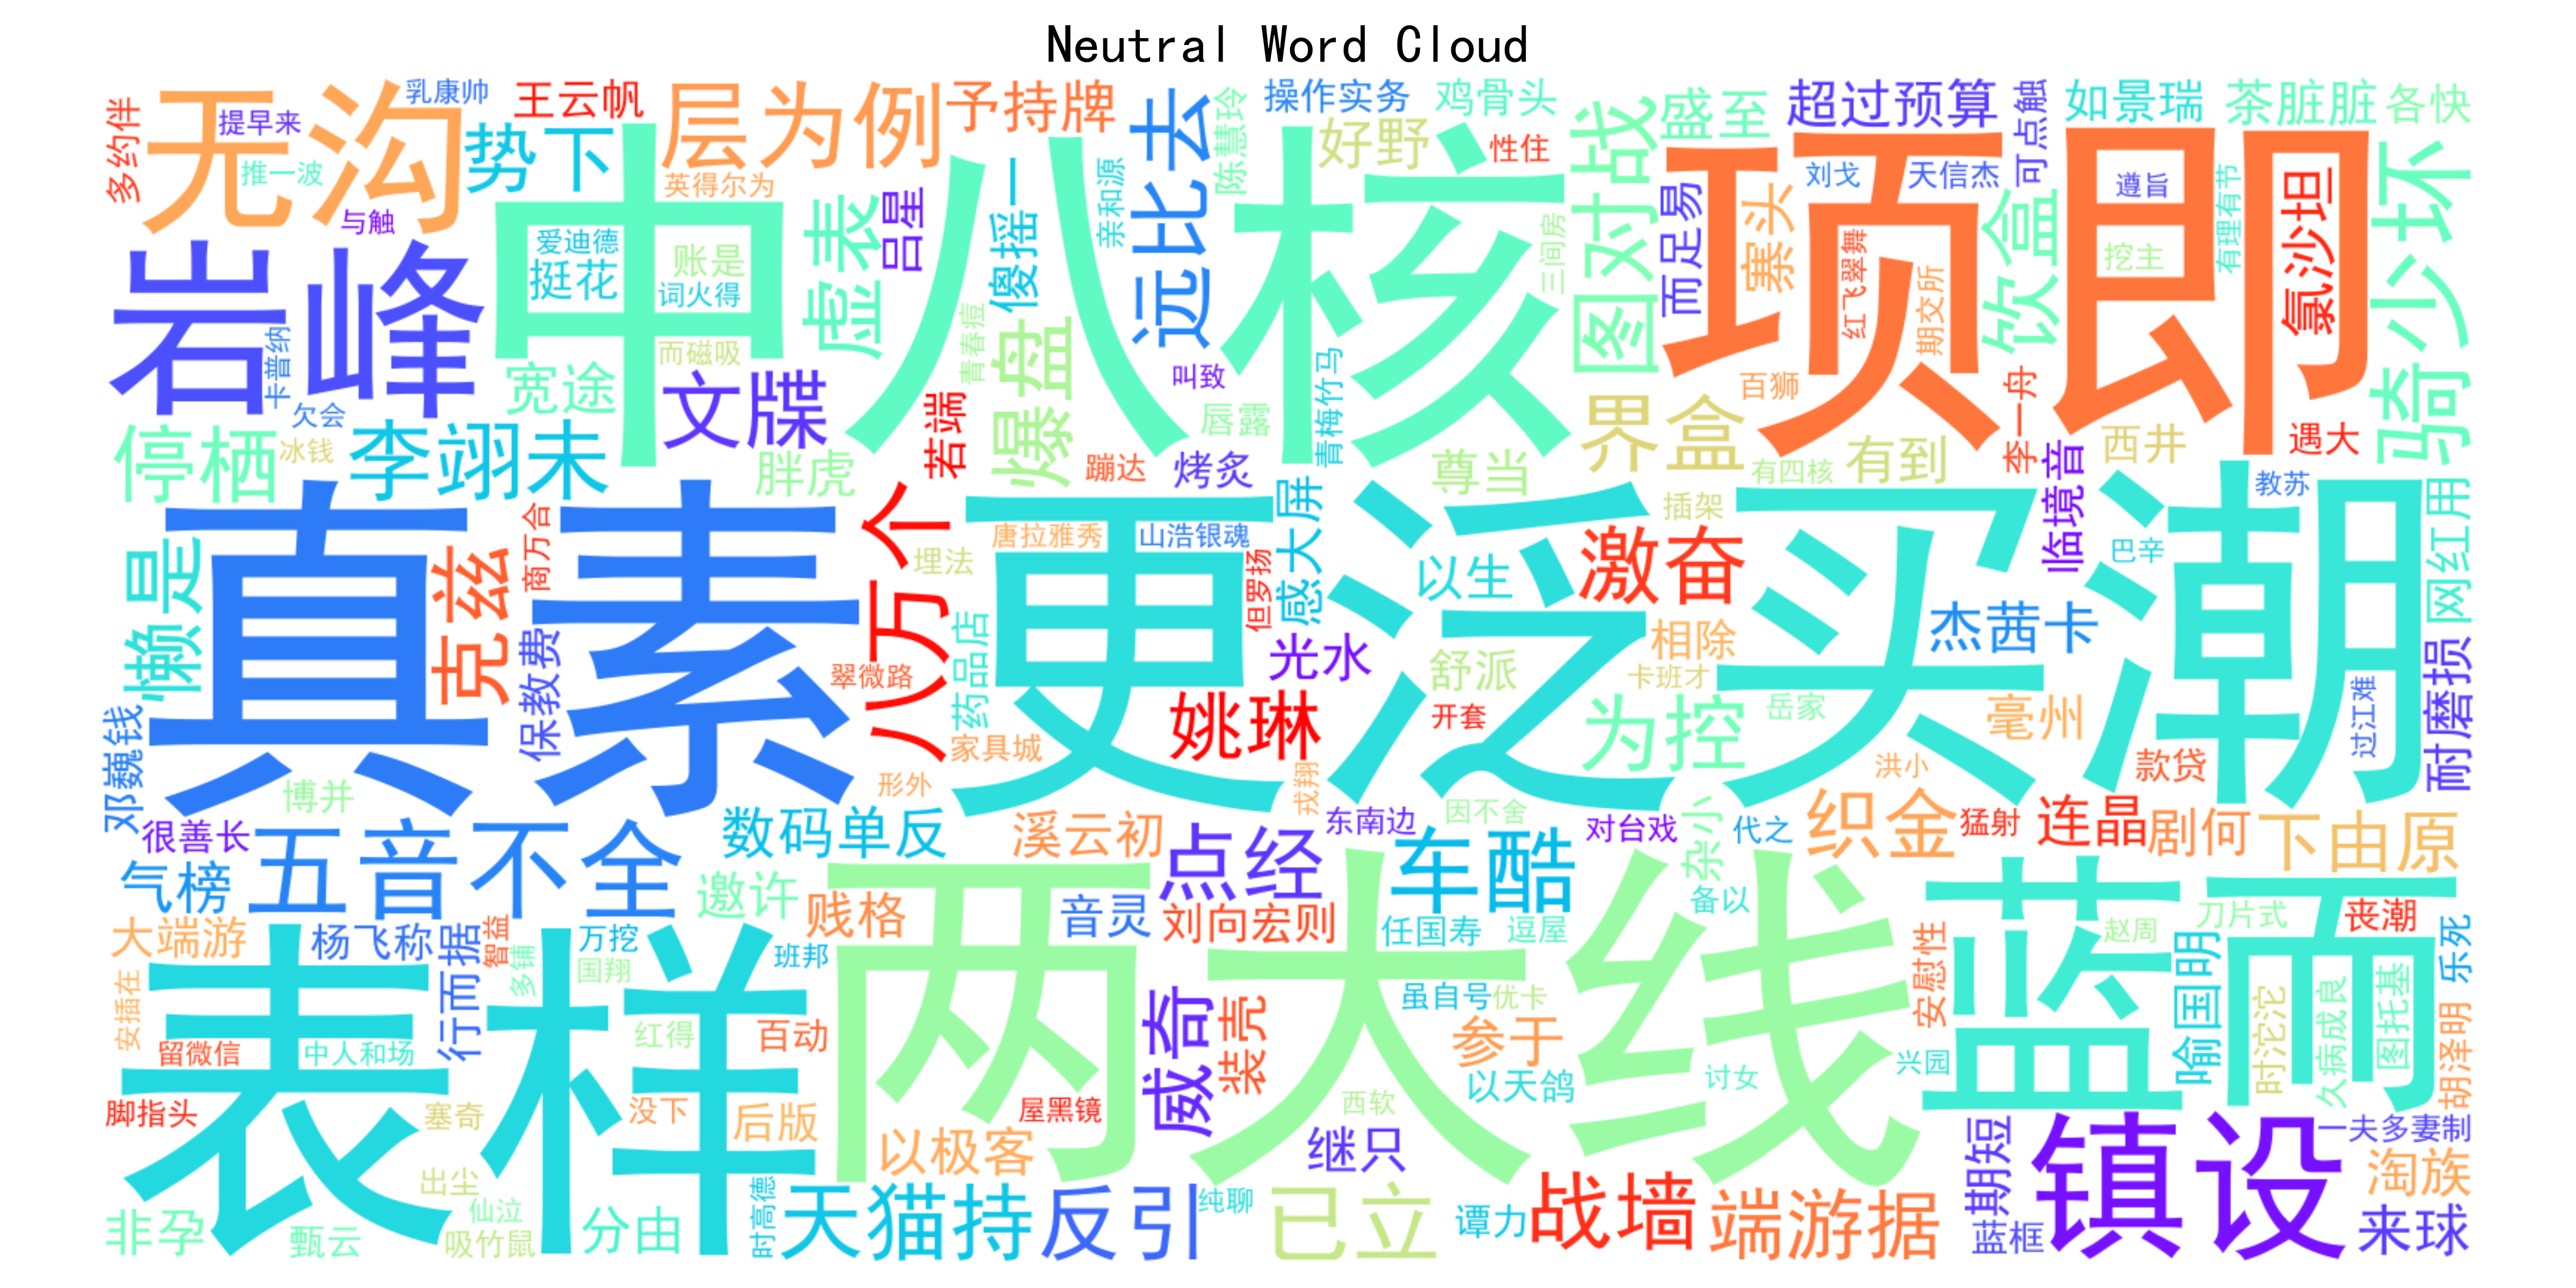
\includegraphics[width=\linewidth]{wordcloud_neutral.png}
		\caption{Word cloud of neutral}
	\end{subfigure}
	\hfill
	\begin{subfigure}[b]{0.32\textwidth}
		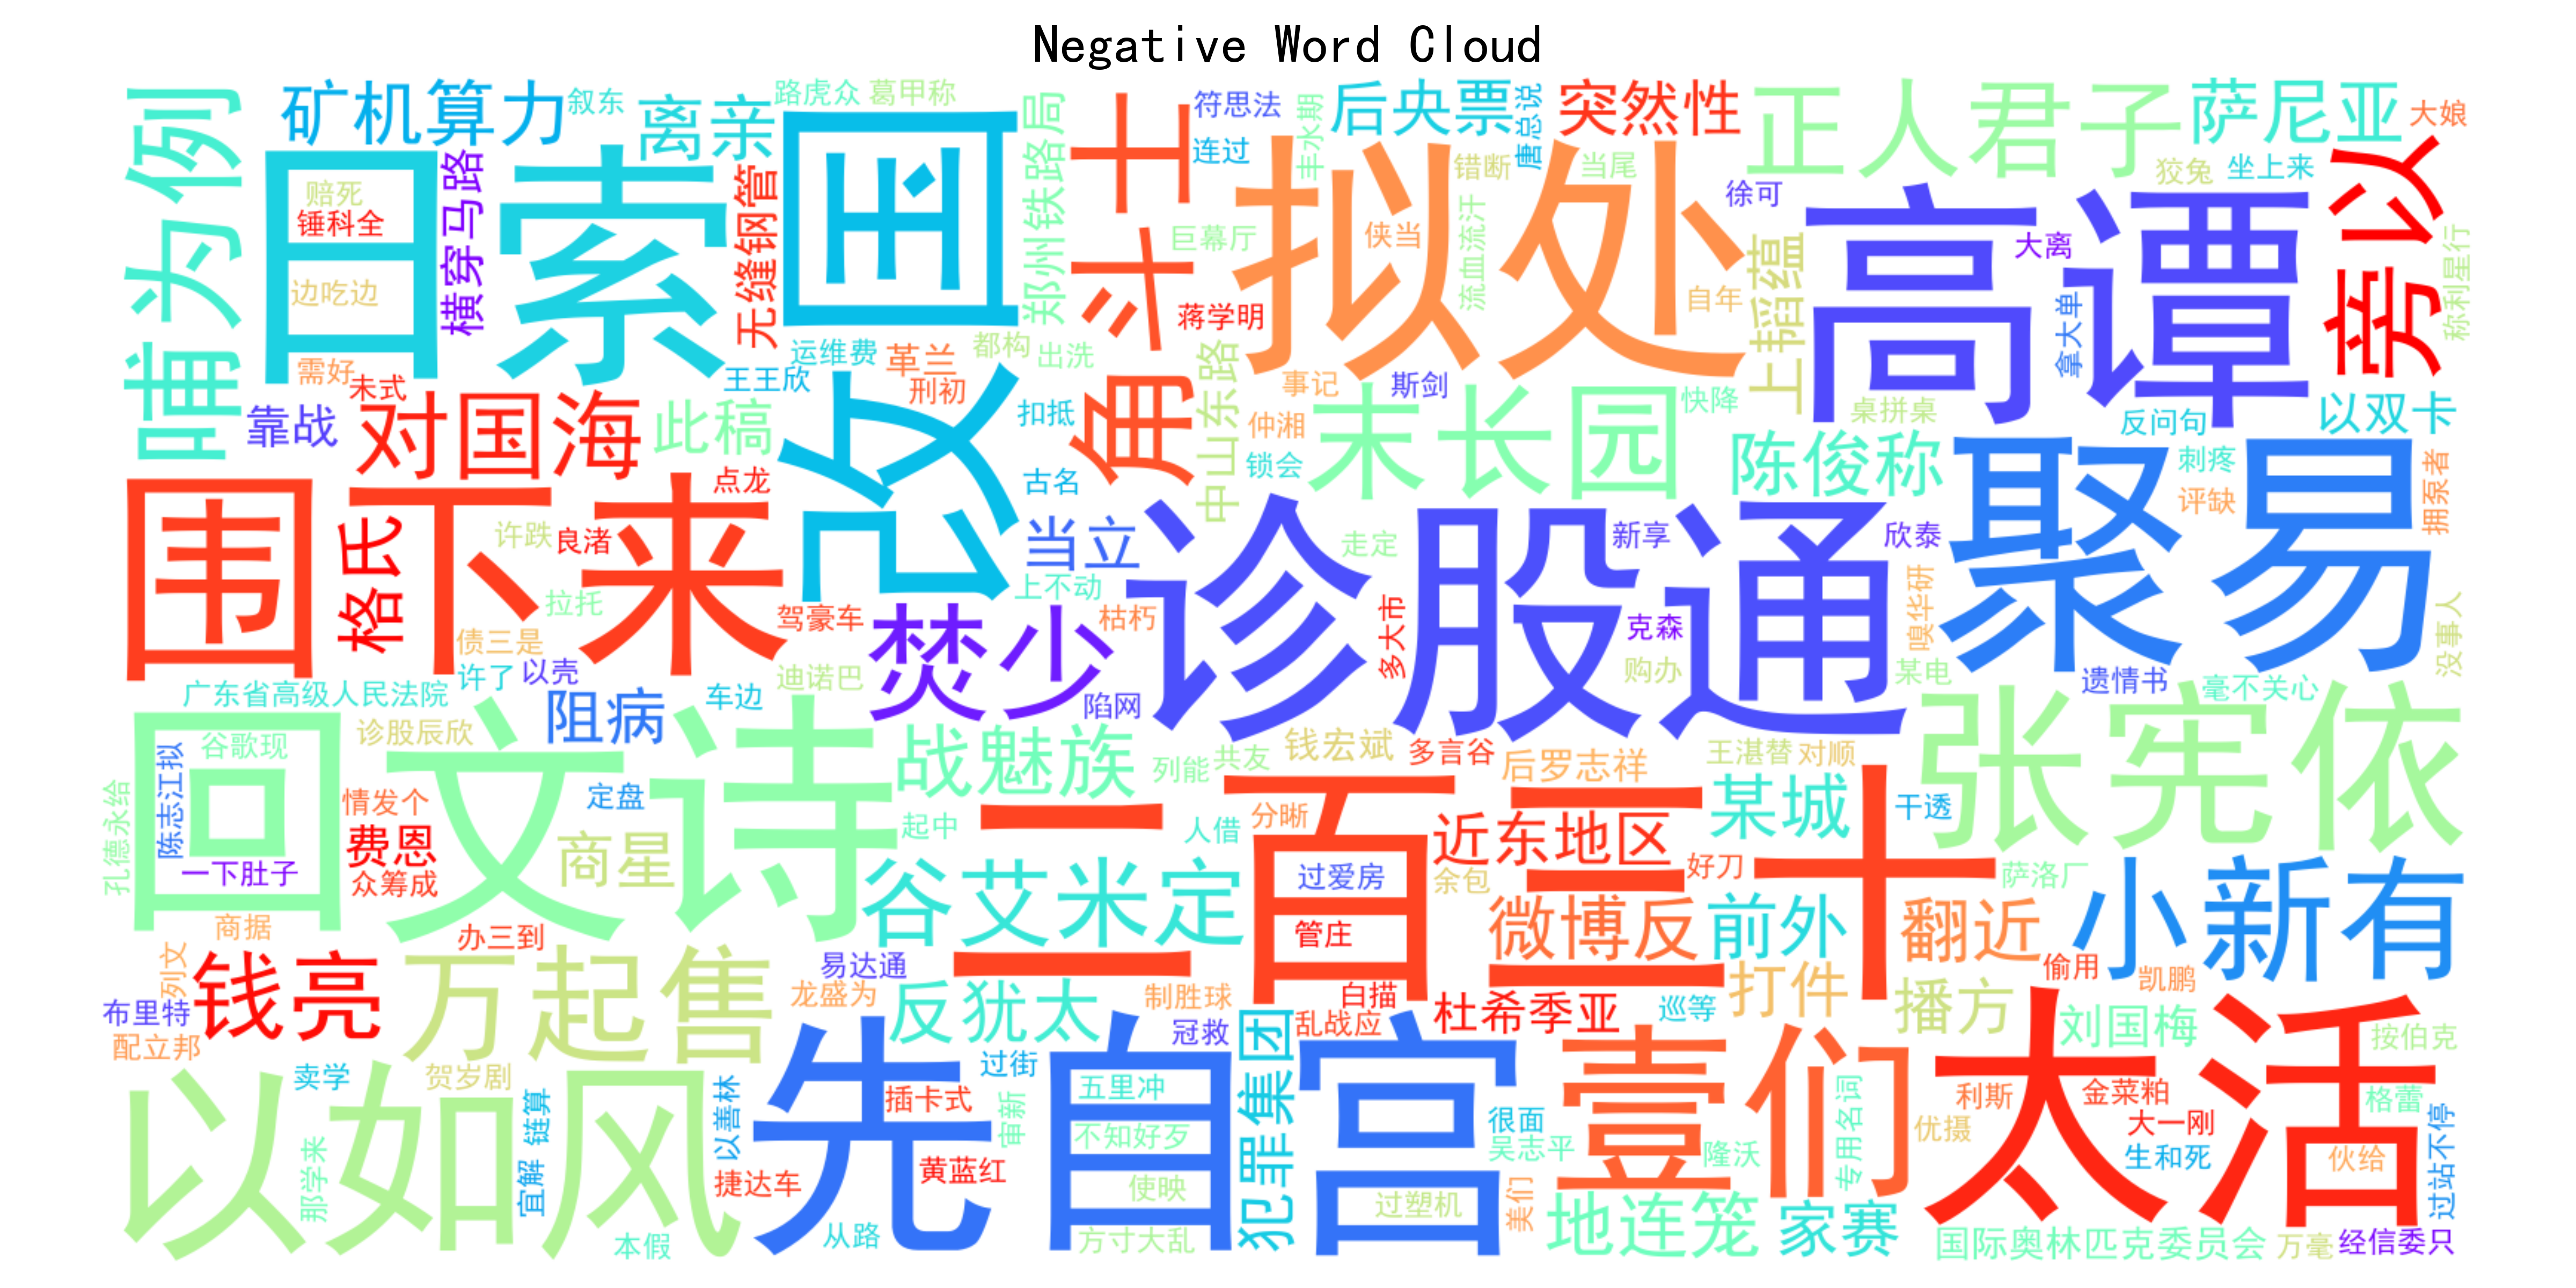
\includegraphics[width=\linewidth]{wordcloud_negative.png}
		\caption{Word cloud of negative}
	\end{subfigure}
	\caption{Word clouds for each sentiment category, illustrating the most frequent words associated with positive, neutral, and negative sentiments. These visualizations highlight the key terms that differentiate the sentiment classes in the dataset.}
	\label{fig:wordclouds}
\end{figure}

\begin{figure}[!ht]
	\centering
	\begin{subfigure}[b]{0.32\textwidth}
		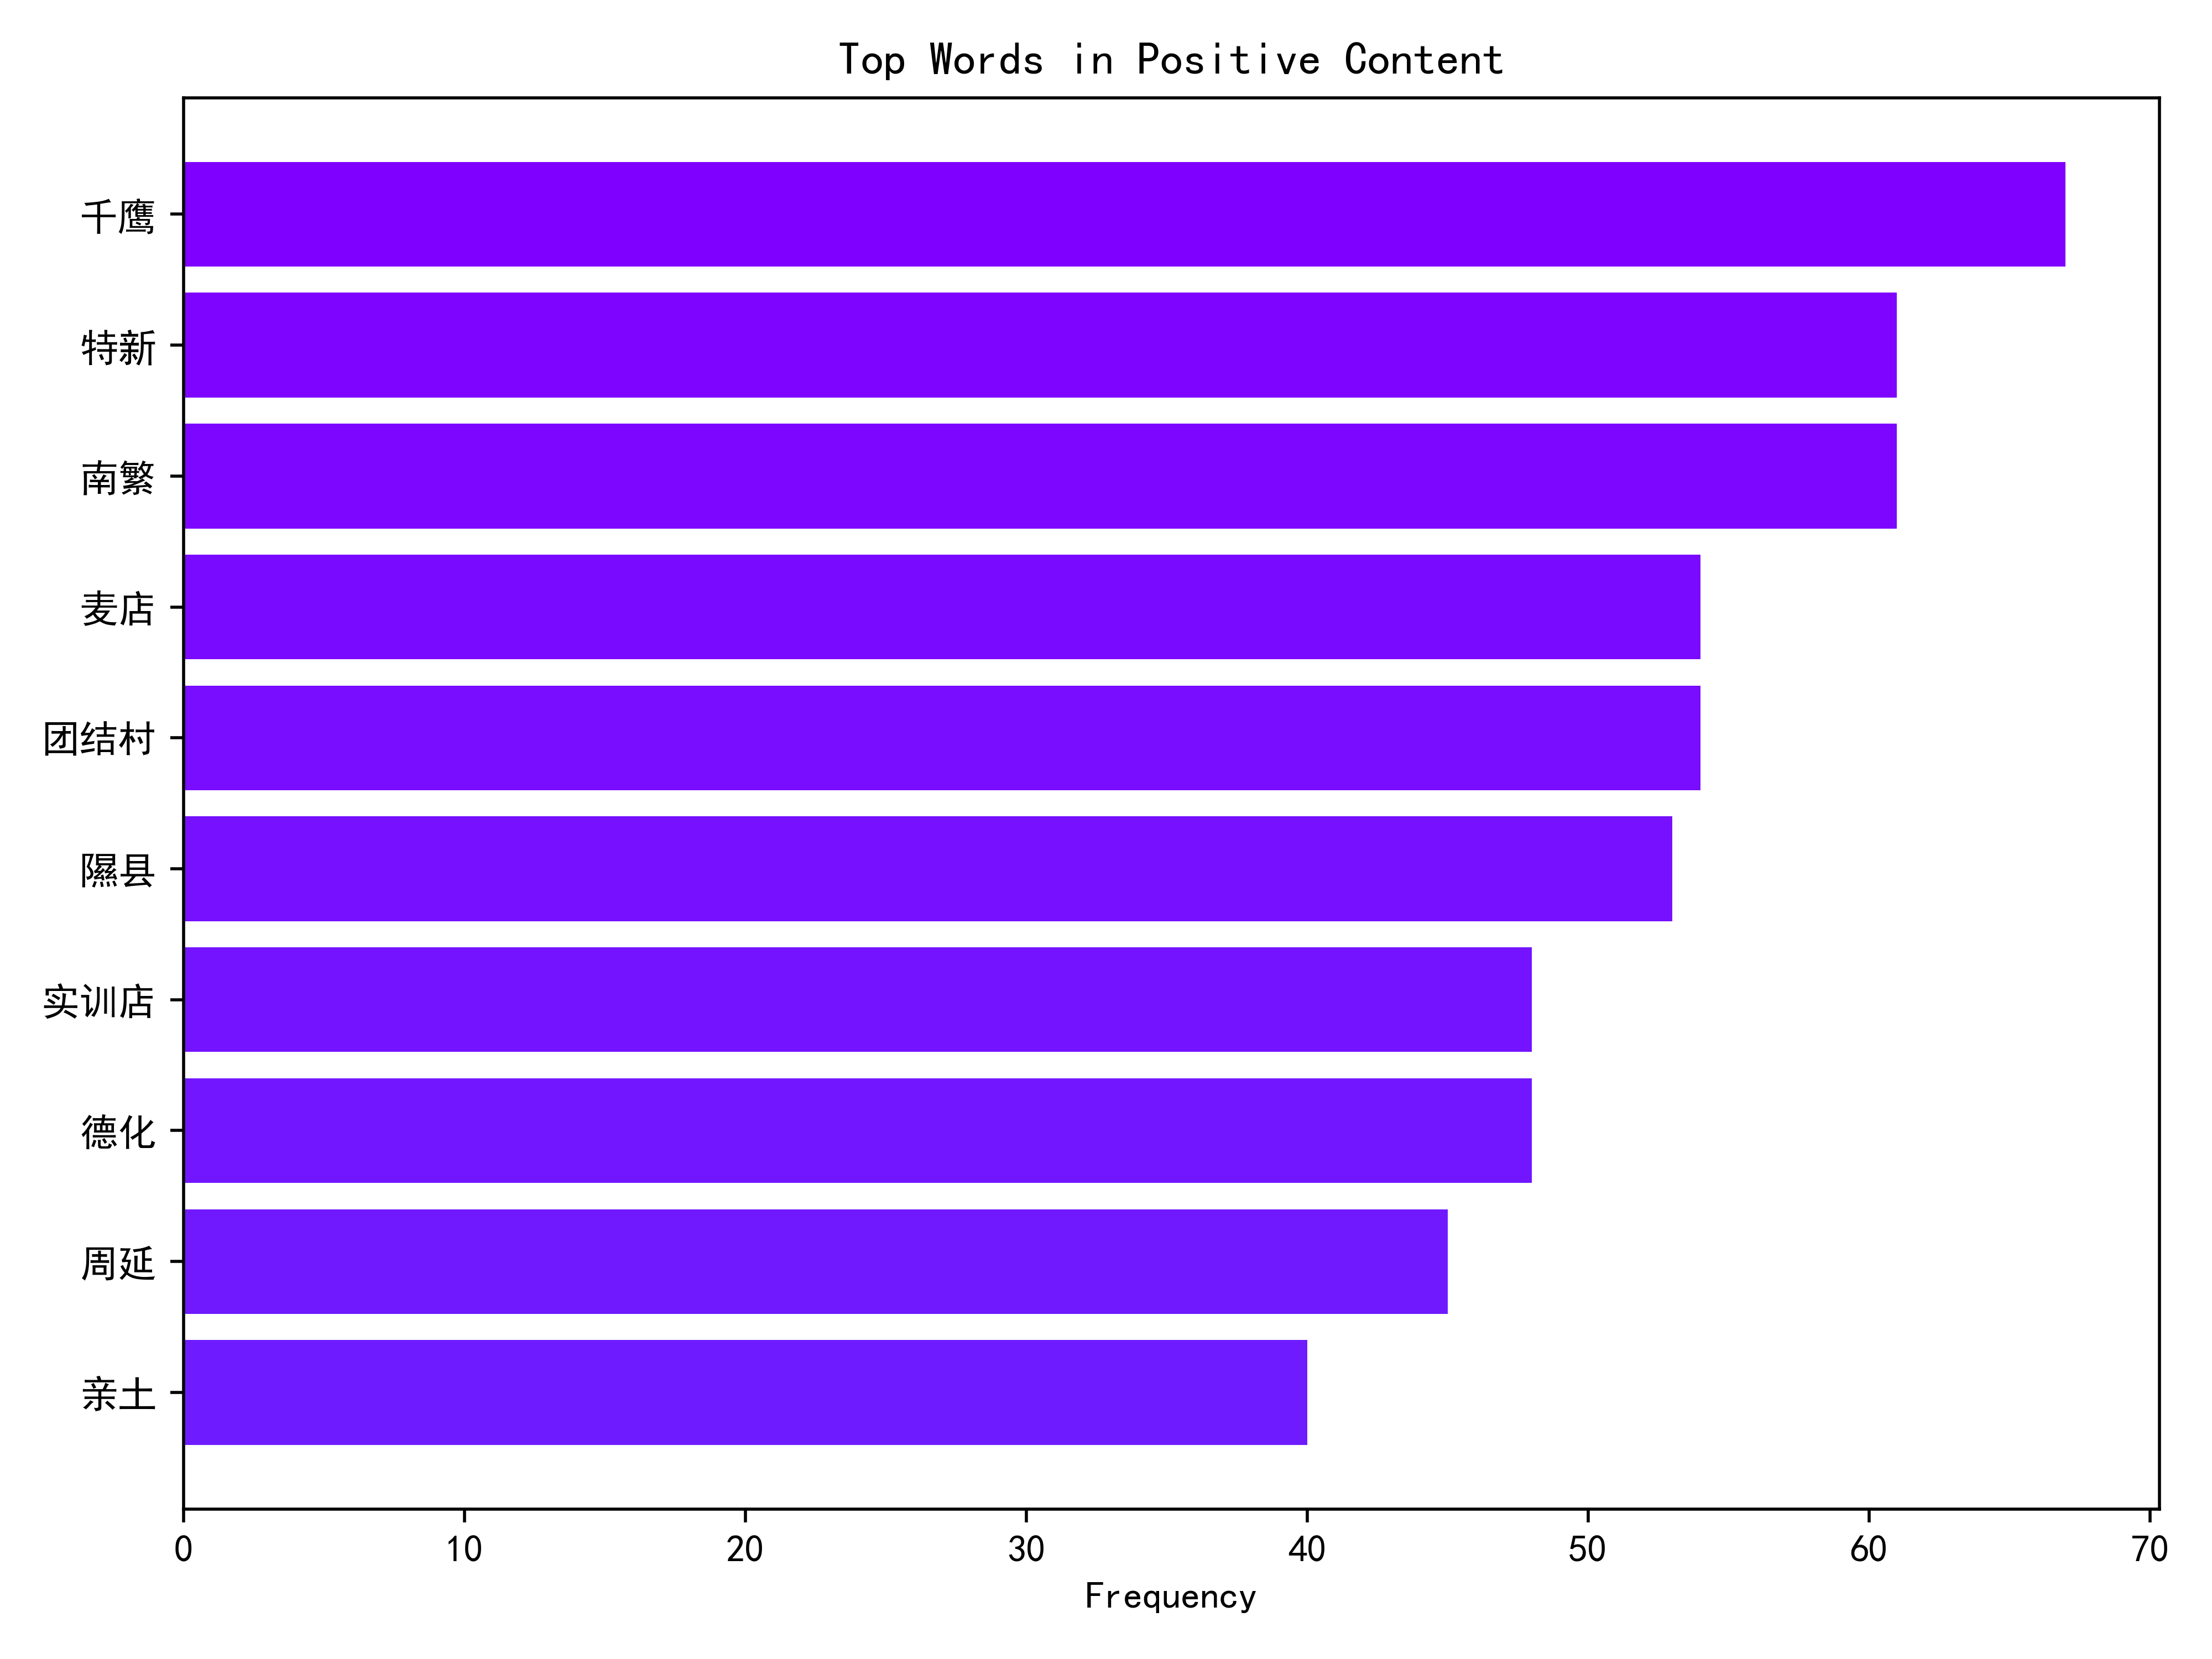
\includegraphics[height=4cm]{top_words_positive.png}
		\caption{Top positive words}
	\end{subfigure}
	\hfill
	\begin{subfigure}[b]{0.32\textwidth}
		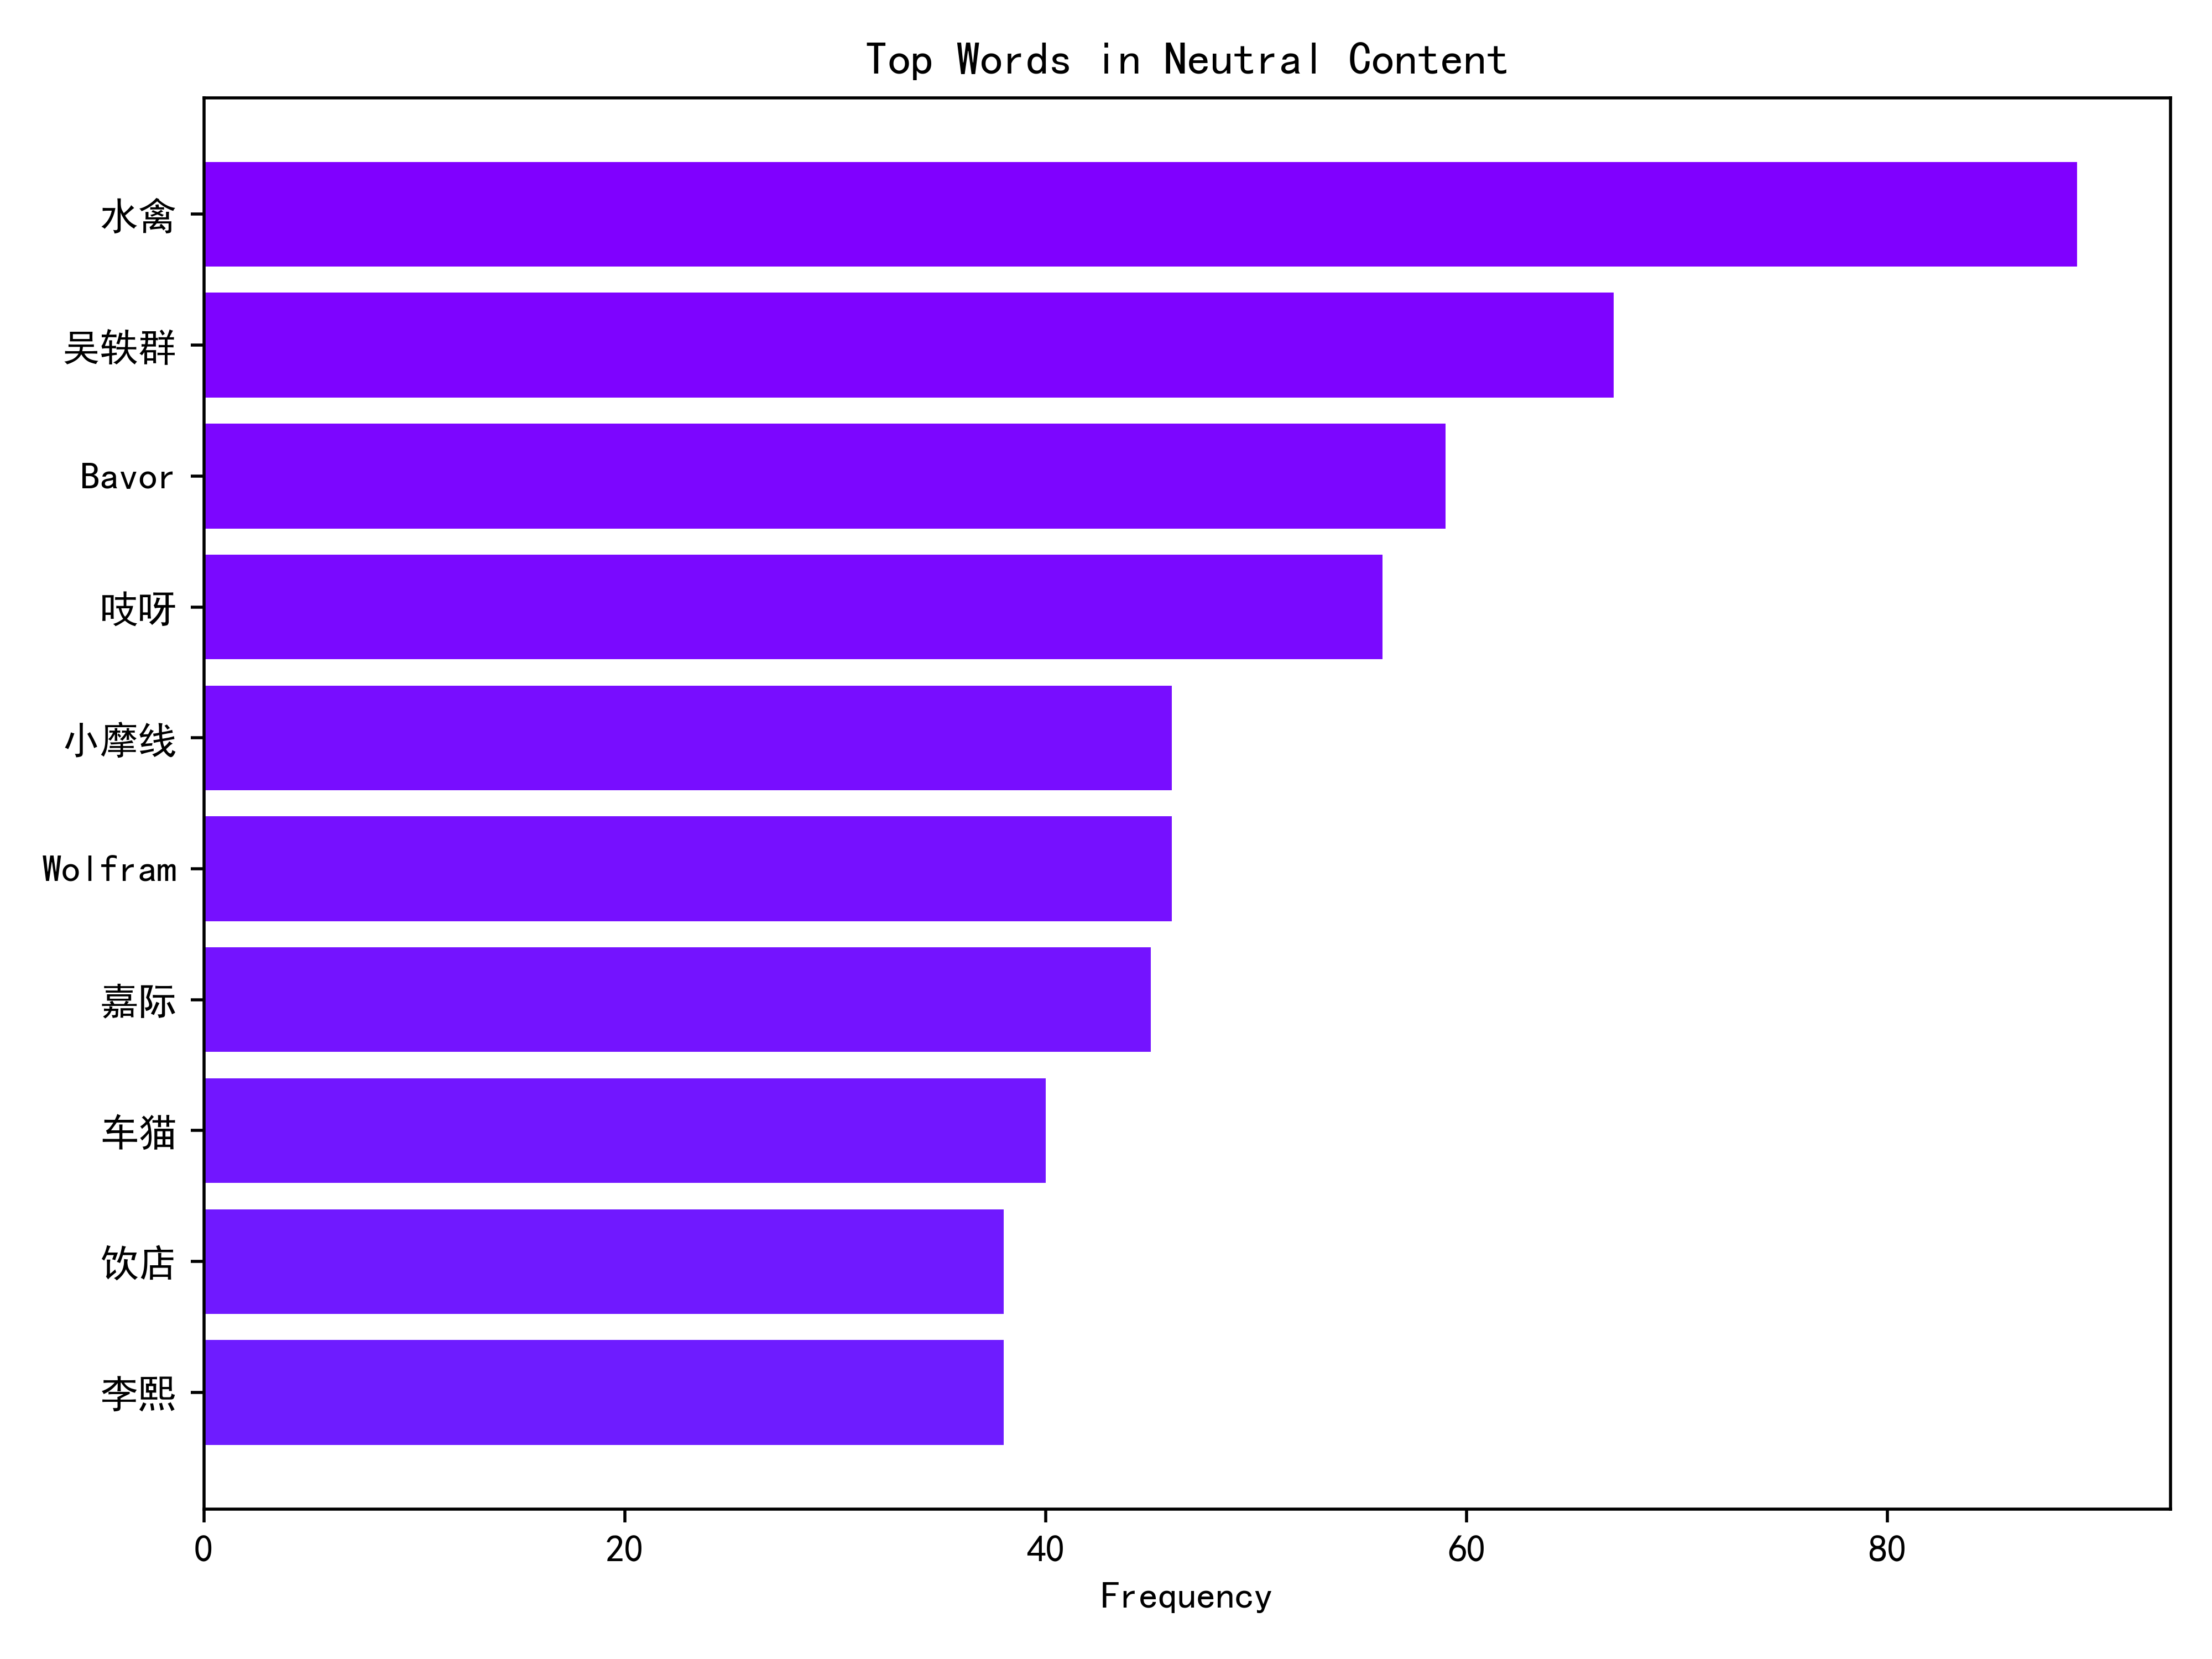
\includegraphics[height=4cm]{top_words_neutral.png}
		\caption{Top neutral words}
	\end{subfigure}
	\hfill
	\begin{subfigure}[b]{0.32\textwidth}
		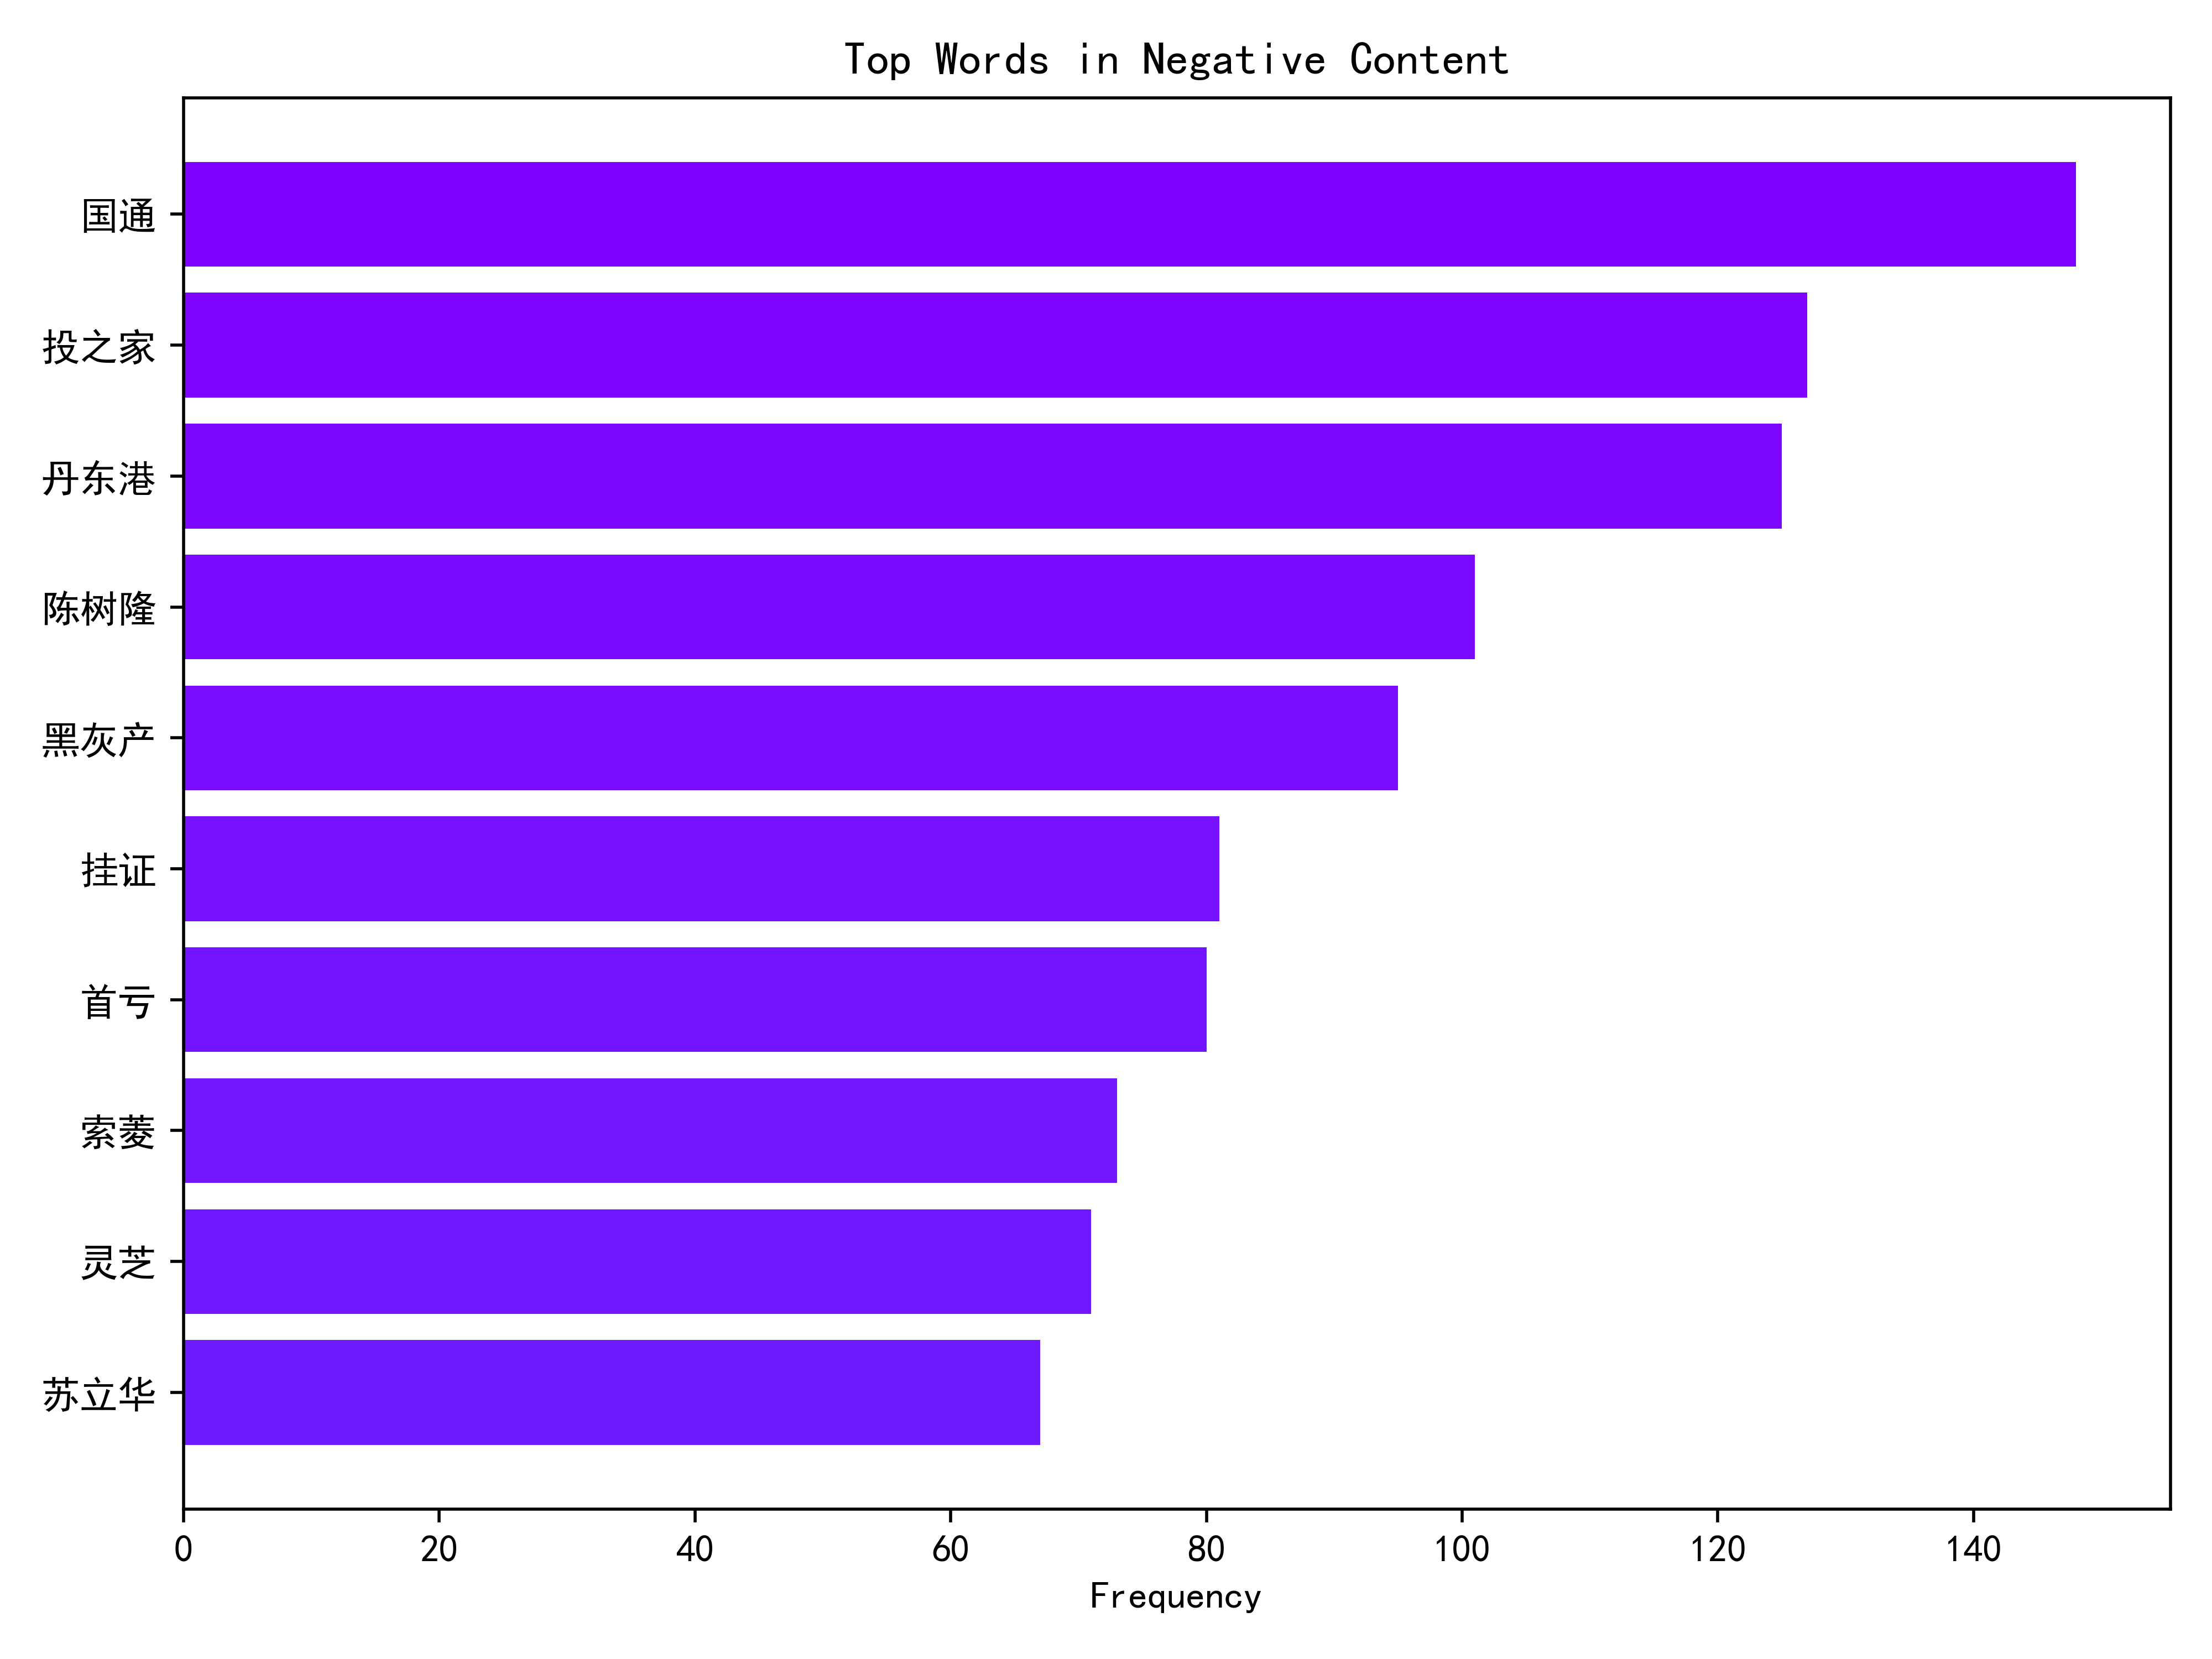
\includegraphics[height=4cm]{top_words_negative.png}
		\caption{Top negative words}
	\end{subfigure}
	\caption{Most frequent words in each sentiment category, showcasing the top terms that contribute to positive, neutral, and negative sentiments. These charts provide insight into the language patterns prevalent in different sentiment classes.}
	\label{fig:top_words}
\end{figure}

\begin{figure}[!ht]
	\centering
	\begin{subfigure}[b]{0.32\textwidth}
		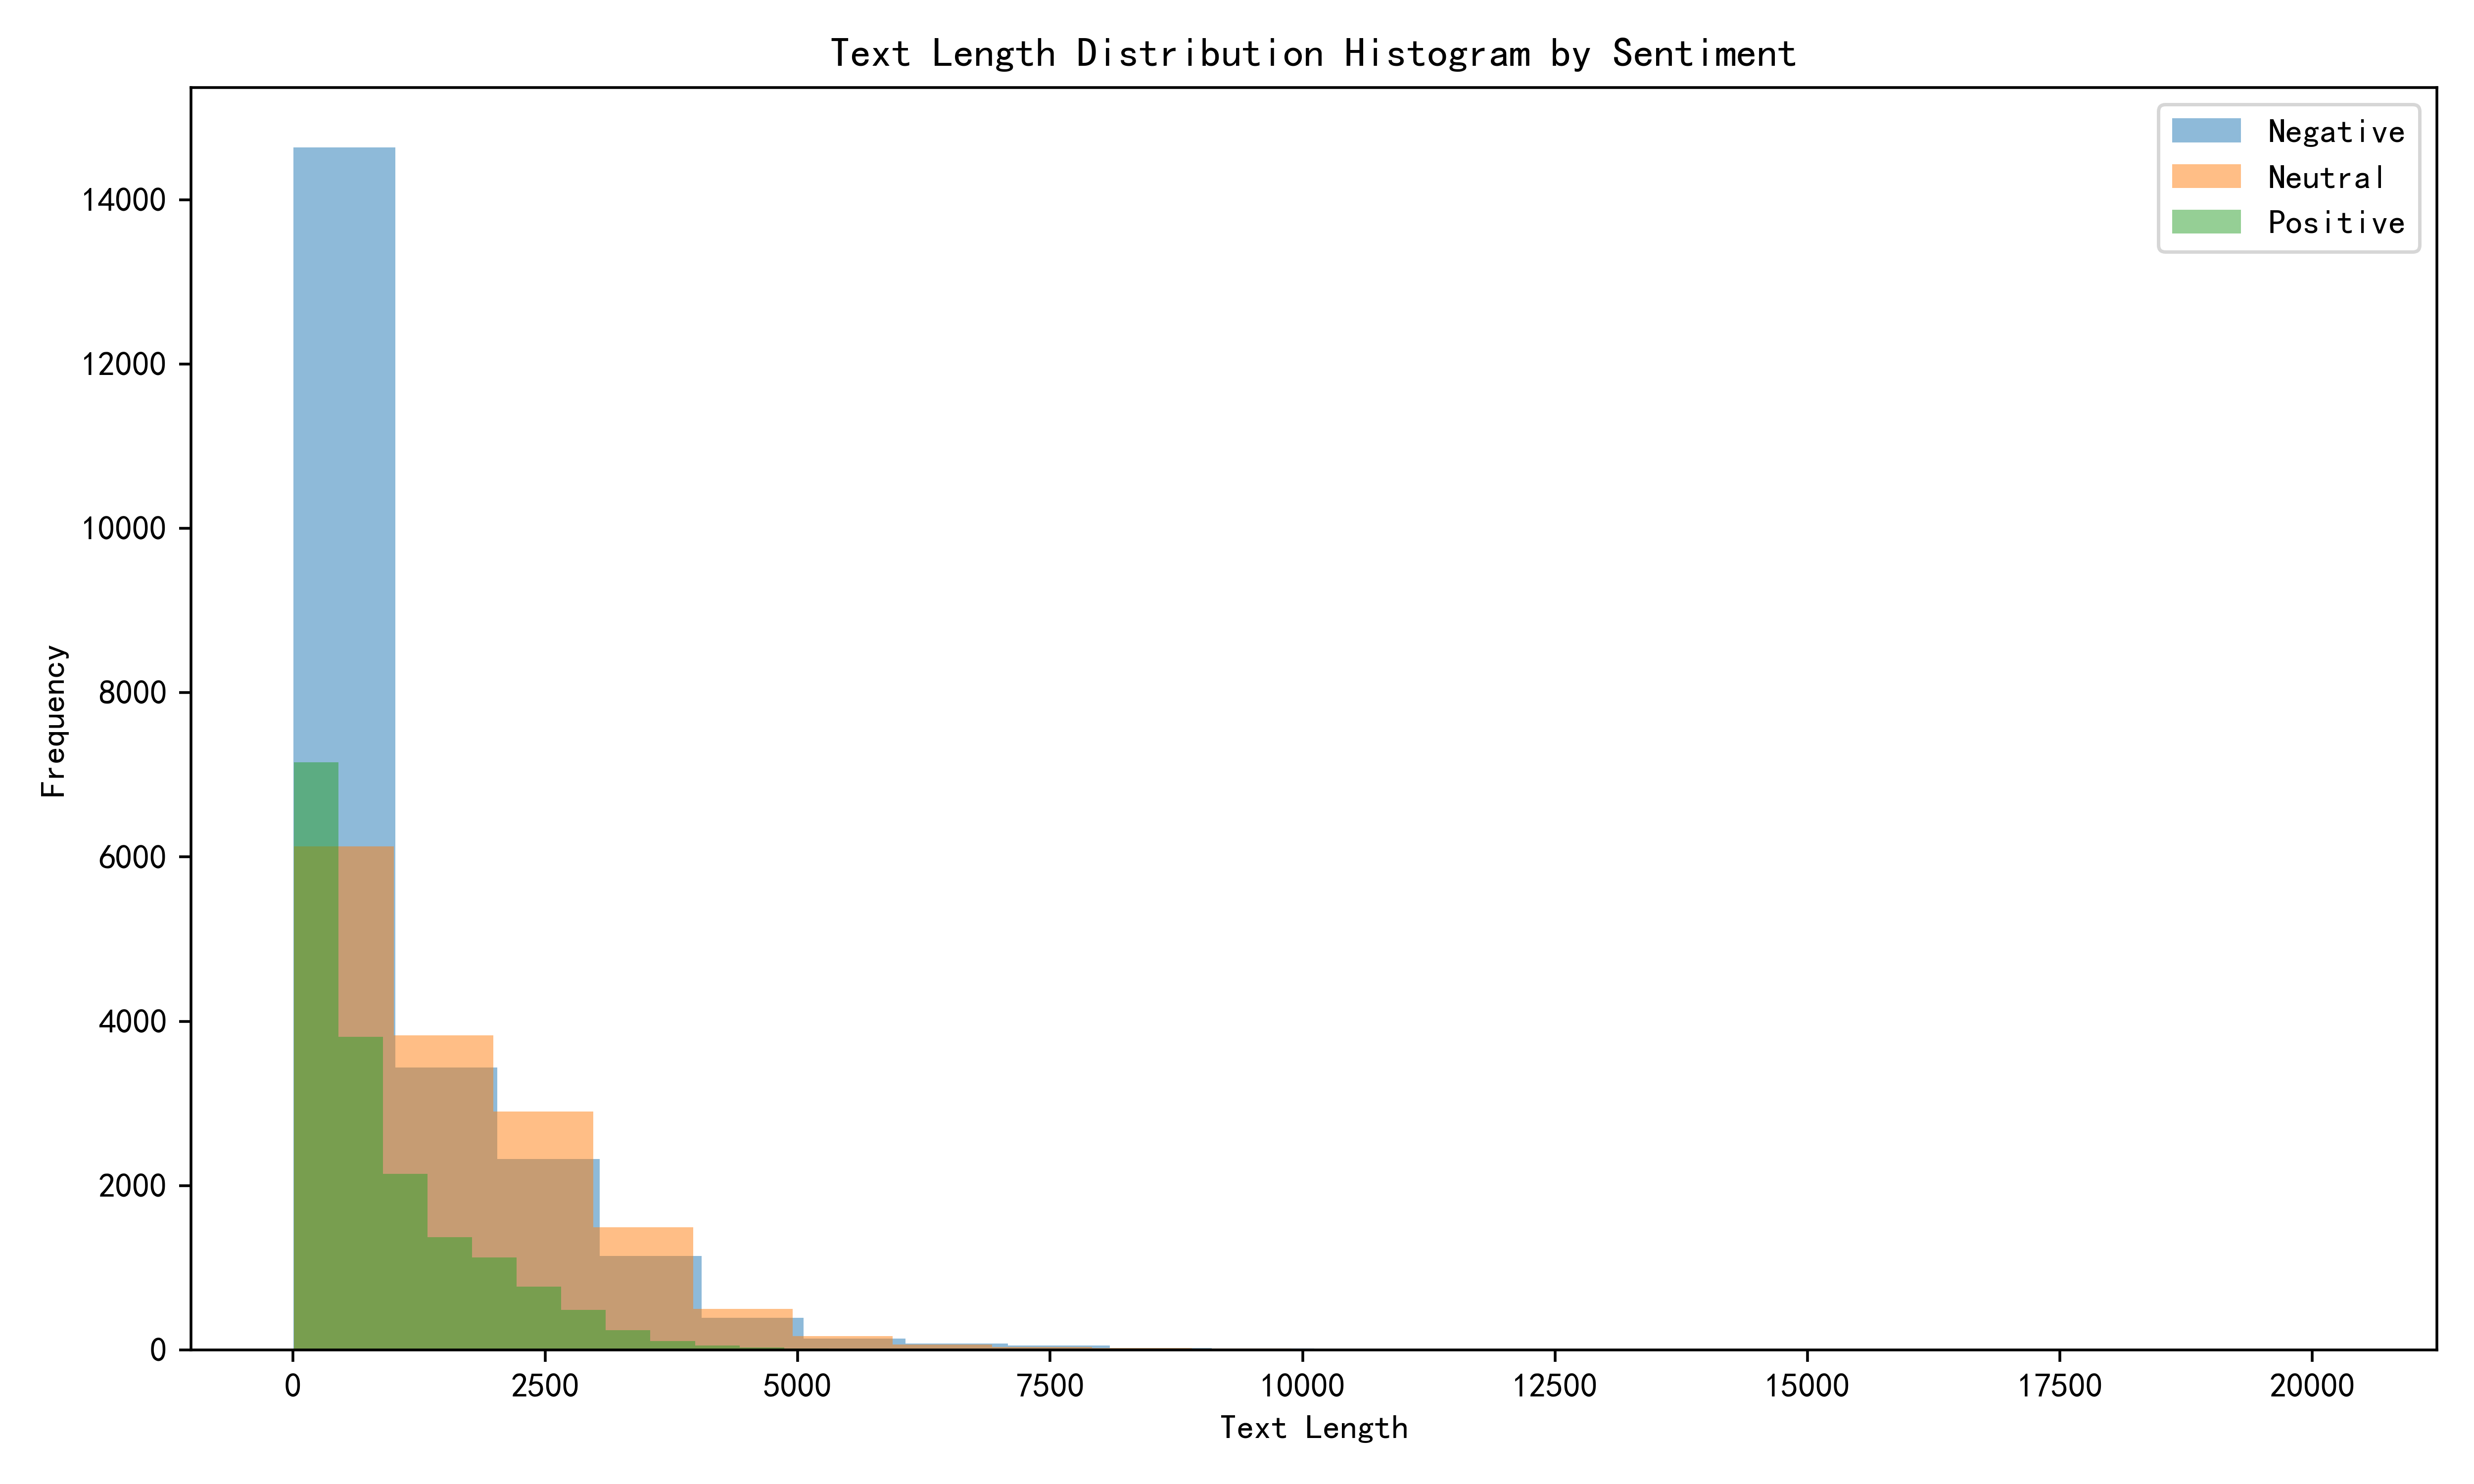
\includegraphics[height=4cm]{text_length_histogram.png}
		\caption{Histogram of text lengths}
	\end{subfigure}
	\hfill
	\begin{subfigure}[b]{0.32\textwidth}
		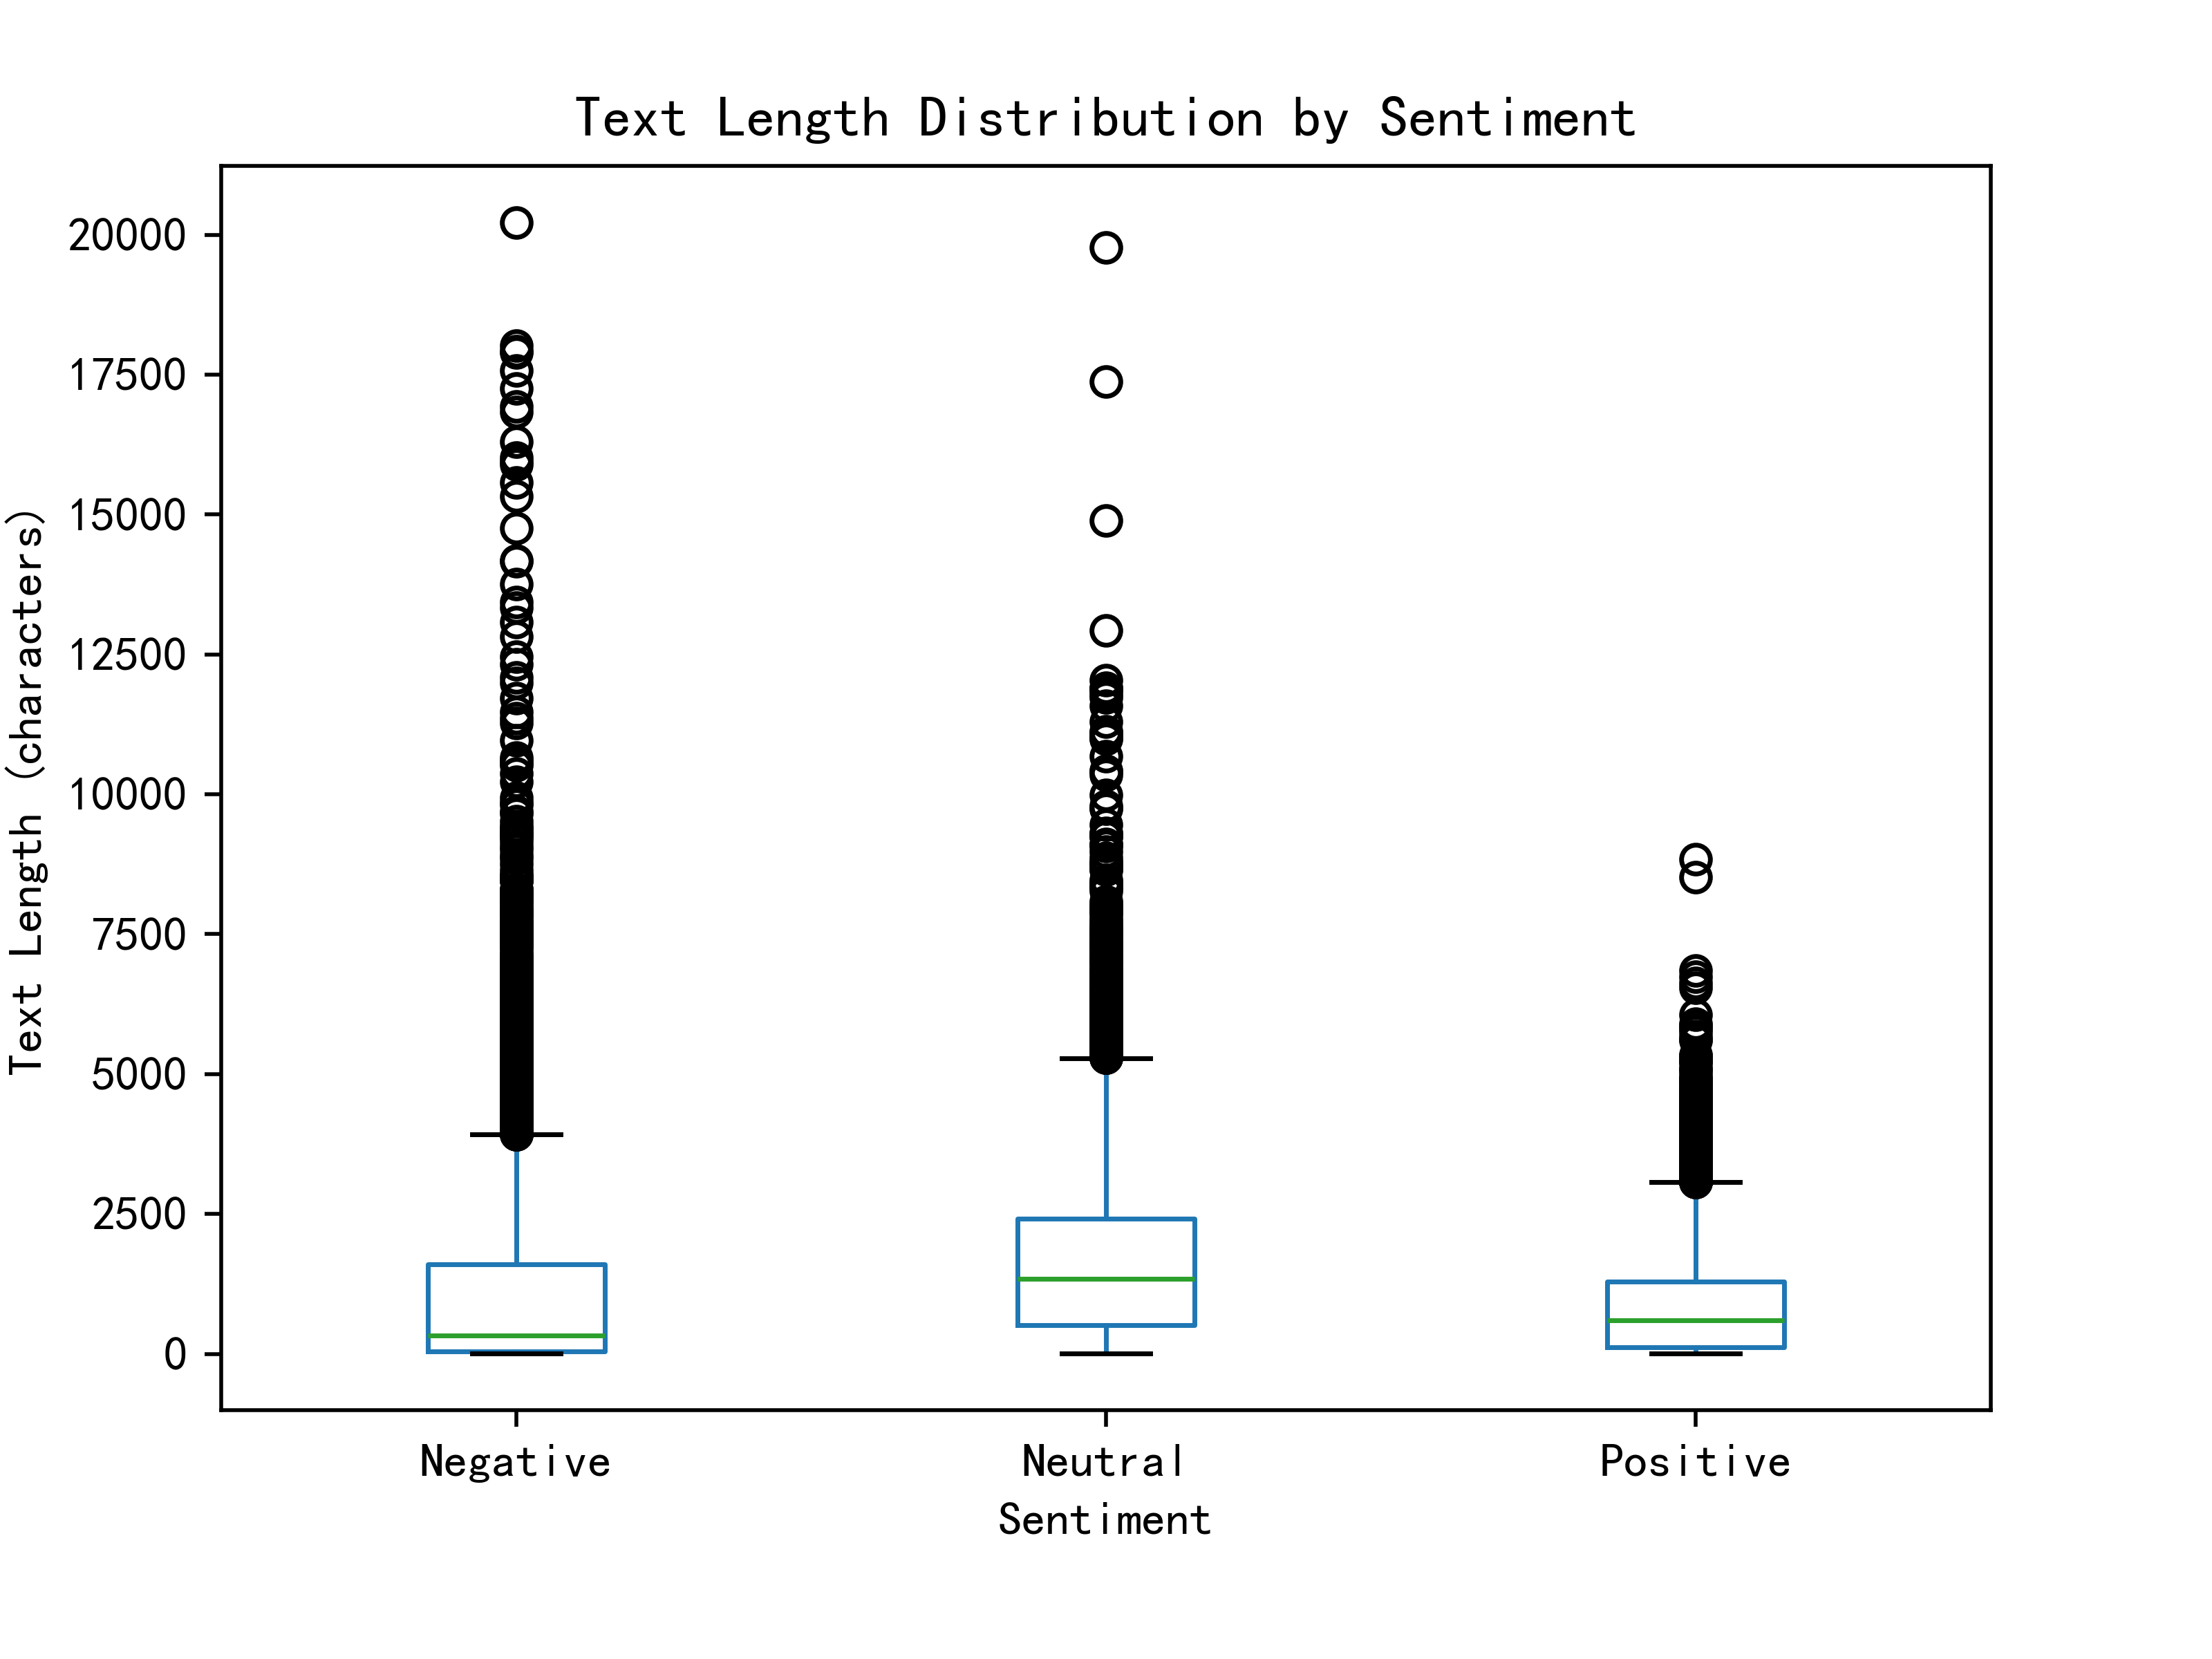
\includegraphics[height=4cm]{text_length_boxplot.png}
		\caption{Boxplot of text lengths}
	\end{subfigure}
	\hfill
	\begin{subfigure}[b]{0.32\textwidth}
		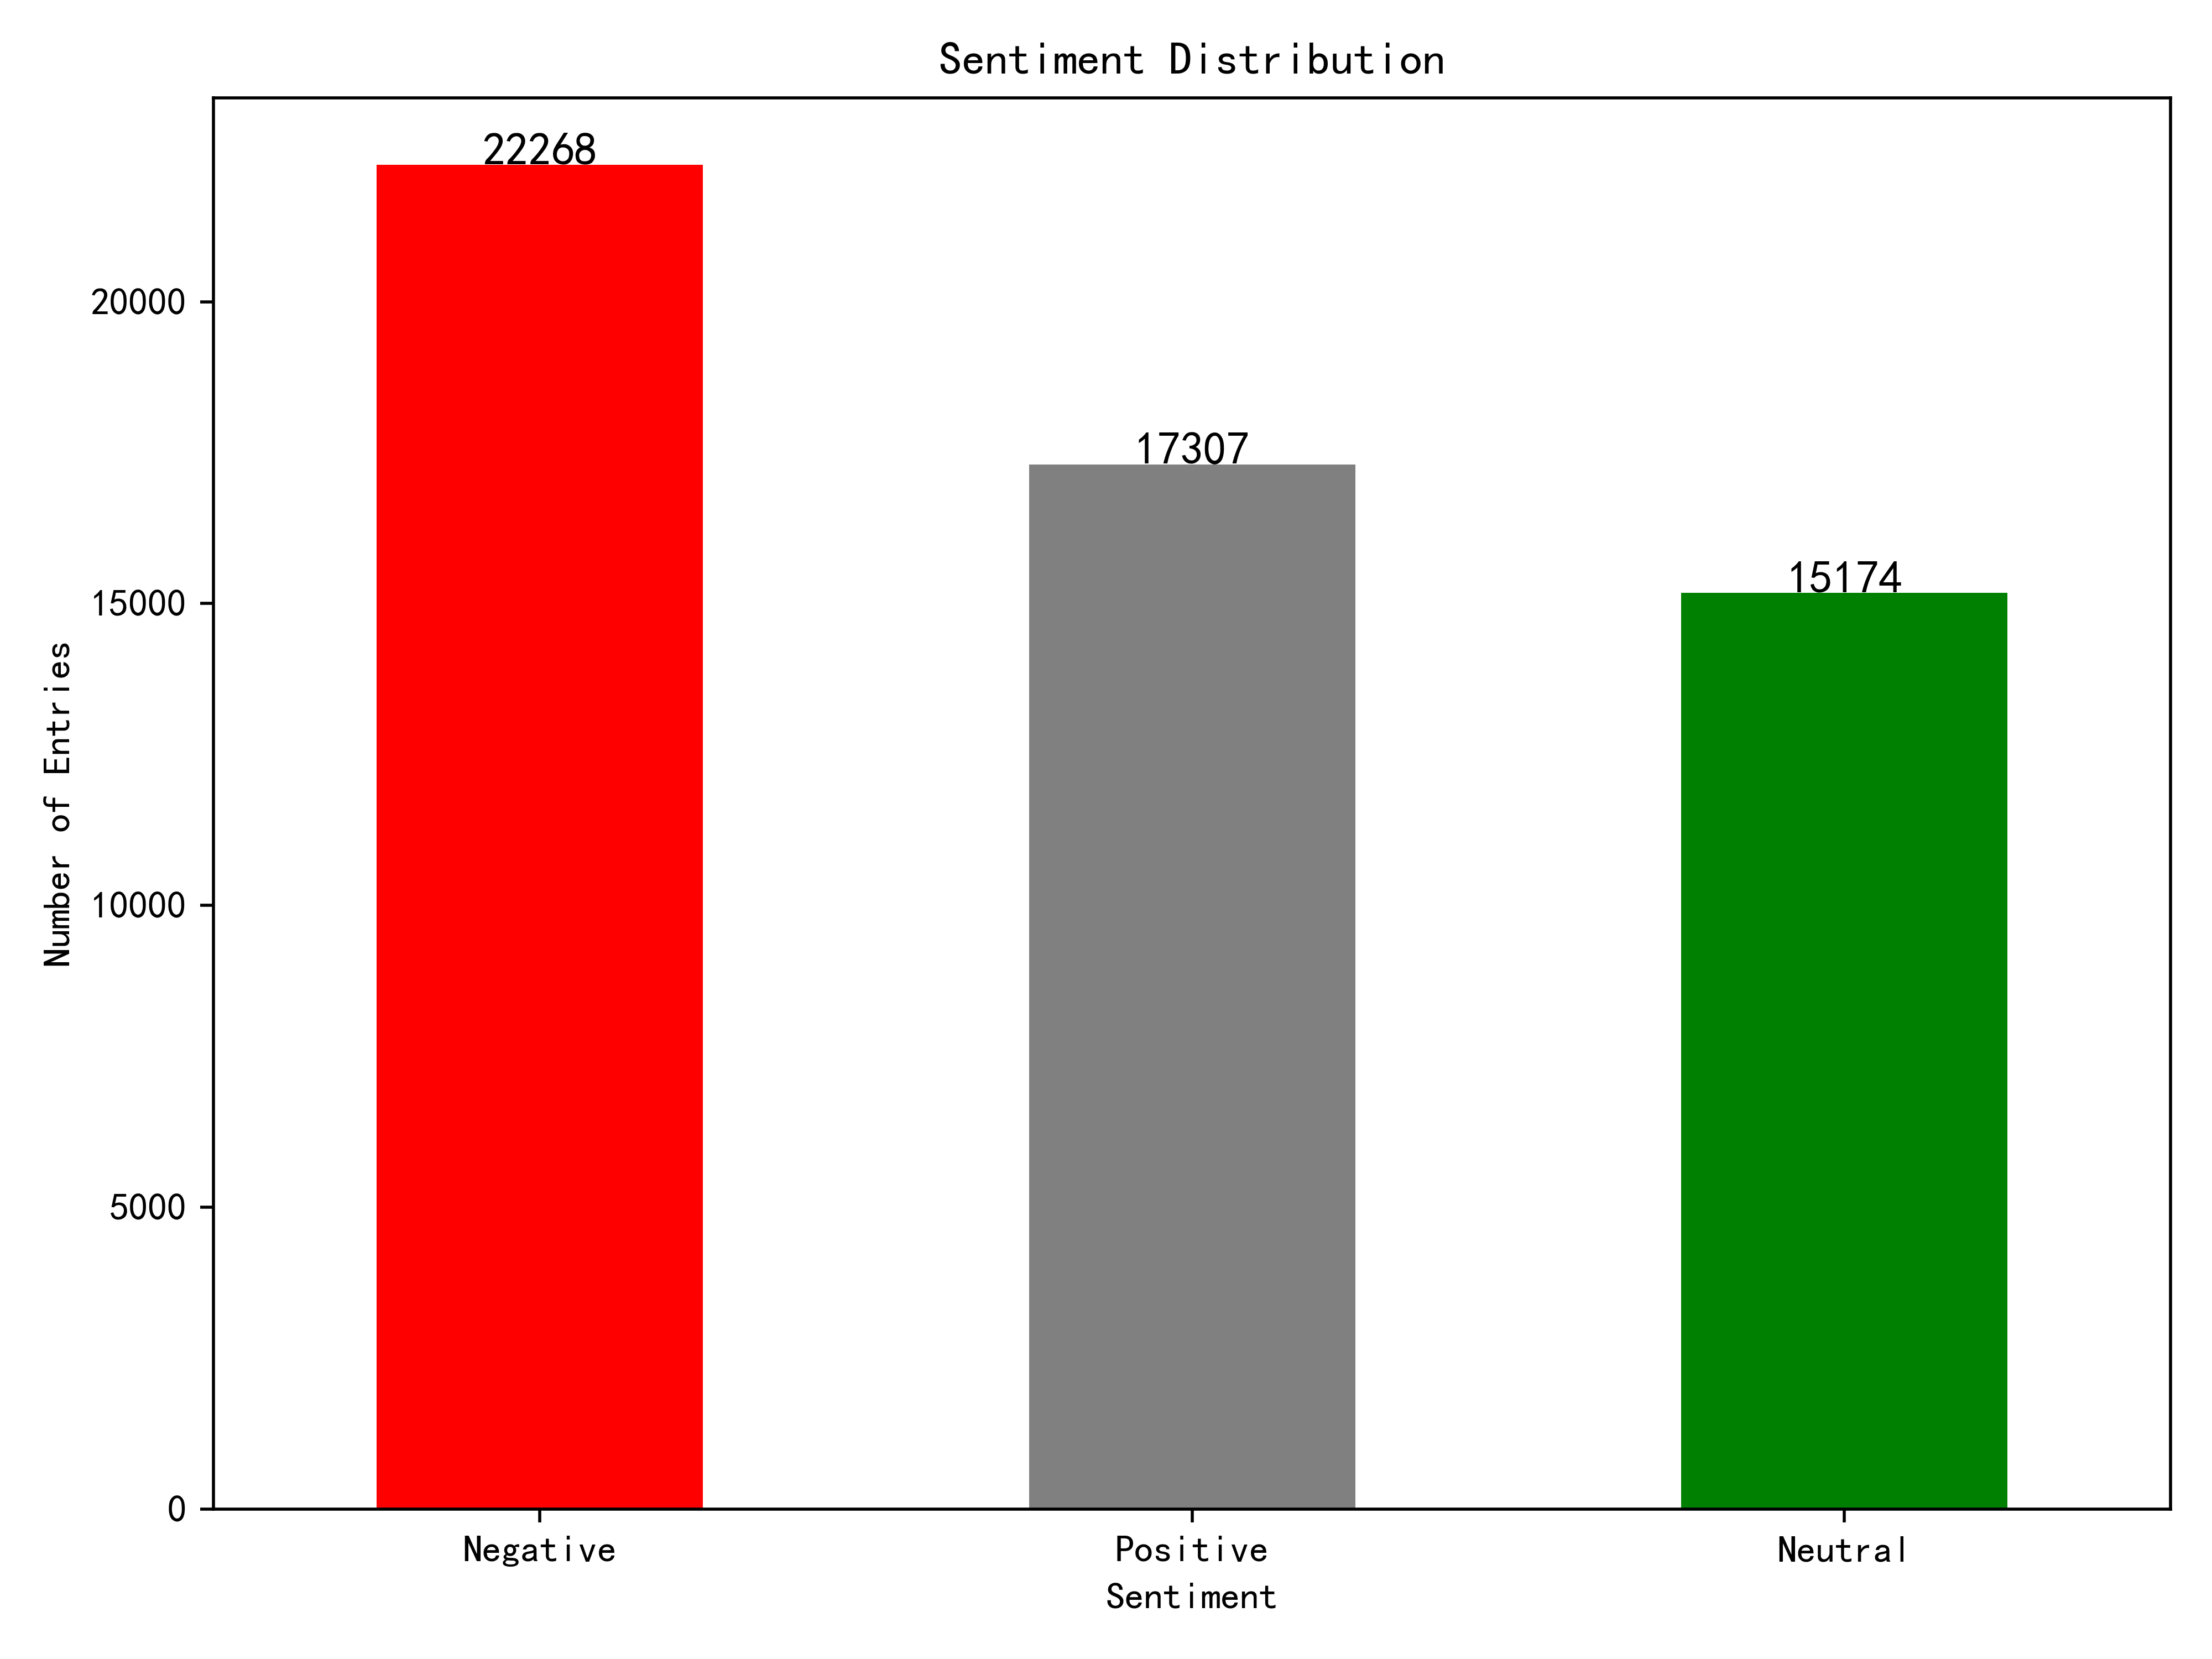
\includegraphics[height=4cm]{sentiment_distribution.png}
		\caption{Sentiment Distribution}
	\end{subfigure}
	\caption{Statistical analysis of the dataset: (a) Histogram displaying the distribution of text lengths, (b) Boxplot illustrating the variability and outliers in text lengths, and (c) Distribution of sentiment categories showing the proportion of positive, neutral, and negative texts. These analyses provide a foundational understanding of the dataset's characteristics.}
	\label{fig:sentiment_distribution}
\end{figure}

\paragraph{Meaningless Chinese Words in Word Clouds}
During word-cloud visualization, several tokens appeared meaningless or out of context. Closer investigation revealed that these originated from awkward translations of specialized English finance terms. This underscores the limitations of our translation approach, wherein certain English words map improperly into Chinese hyperspace, yielding unnatural tokens that nonetheless appear in frequency-based visualizations.


\subsection{Lexicon-Based Annotation}

Lexicon-based annotation matches words or phrases from a predefined dictionary to text segments and assigns associated sentiment scores. Jiang et al. \cite{ref3, ref4} proposed a Chinese financial sentiment lexicon that In the Chinese financial domain, terminologies and colloquialisms evolve rapidly, complicating this step. Yet, even partial coverage by a domain-specific lexicon can significantly accelerate the annotation process. 

\subsection{Model Training}
\subsubsection{TNMT for Corpus Expansion}
\label{subsec:TNMTperf}
We trained a TNMT model to translate English financial texts into Chinese. Evaluated using BLEU scores and F1 metrics, the model effectively enlarged our Chinese dataset. However, some translated words remain semantically mismatched. Future enhancements could involve domain-specific dictionaries or graph-based mapping approaches to reduce translation noise.

\subsubsection{BERT Fine-Tuning}
Our main classification model builds upon a pre-trained Chinese BERT. We fine-tuned it by feeding the annotated data as input, monitoring metrics like accuracy, F1 score, and training loss. While BERT generally outperforms older generation RNN-based methods, traditional or Bayesian models may, in certain scenarios with less data or higher interpretability demands, provide more transparent and sometimes even superior performance.

The whole algorithm pipeline is illustrated in Figure \ref{fig:pipeline}.\

\begin{figure}[!ht]
	\centering
	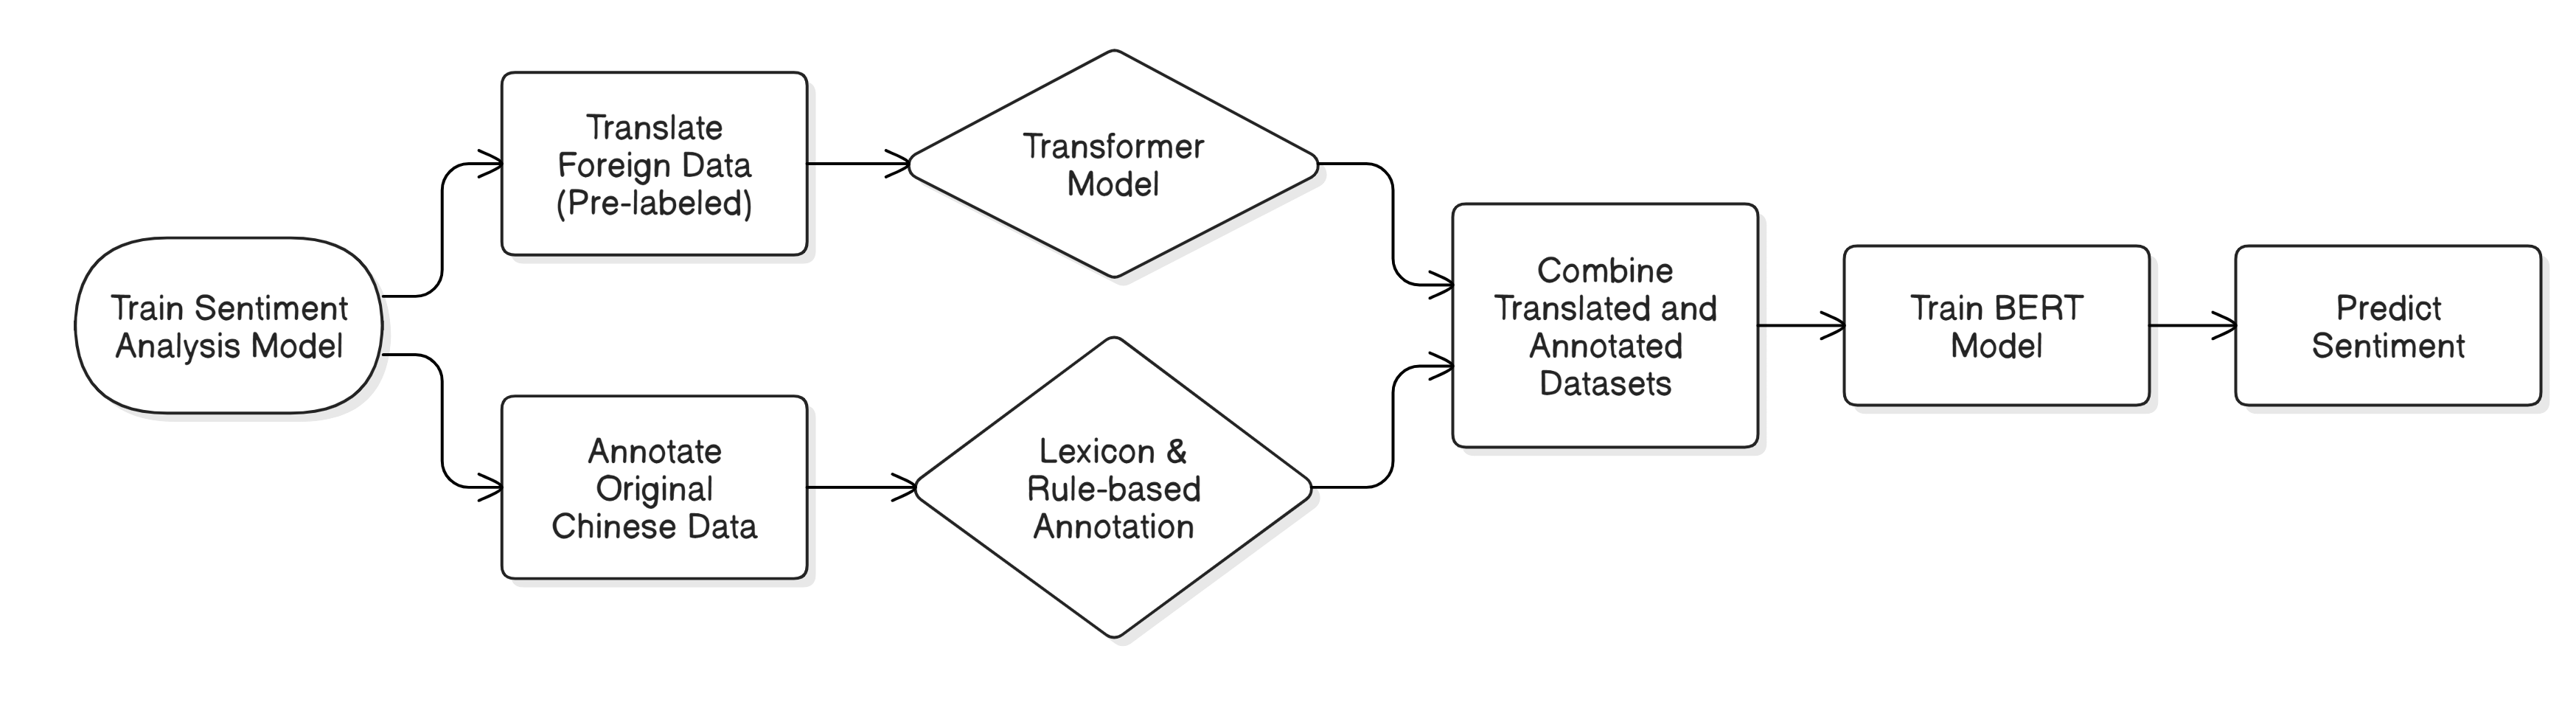
\includegraphics[width=\textwidth]{pipeline.png}
	\caption{Algorithm pipeline for Chinese financial sentiment analysis. The workflow encompasses data collection, translation, lexicon-based annotation, and model training.}
	\label{fig:pipeline}
\end{figure}

%----------------------------------------
% 4. EXPERIMENTS AND RESULTS
%----------------------------------------
\section{Experiments and Results}
\label{sec:results}

\subsection{Transformer-Based Translation}
Figures~\ref{fig:tnmt_performance} shows the training loss, evaluation BLEU score, F1 score, accuracy, precision, and recall of the TNMT model over 350 steps. The model exhibits a steady decline in training loss and a corresponding increase in evaluation BLEU, F1, and accuracy. Precision and recall curves also show consistent improvement, indicating the model's ability to capture nuanced sentiment cues in the translated texts. However, the presence of "meaningless" tokens in word clouds suggests that the model may struggle with specialized financial terminology, necessitating further refinement. Furthermore, although the performance metrics show improvement, the model's overall accuracy and F1 score remain suboptimal, indicating the need for additional enhancements.

% Model Performance Over 350 Steps
\begin{figure}[!ht]
	\centering
	\begin{subfigure}[b]{0.32\textwidth}
		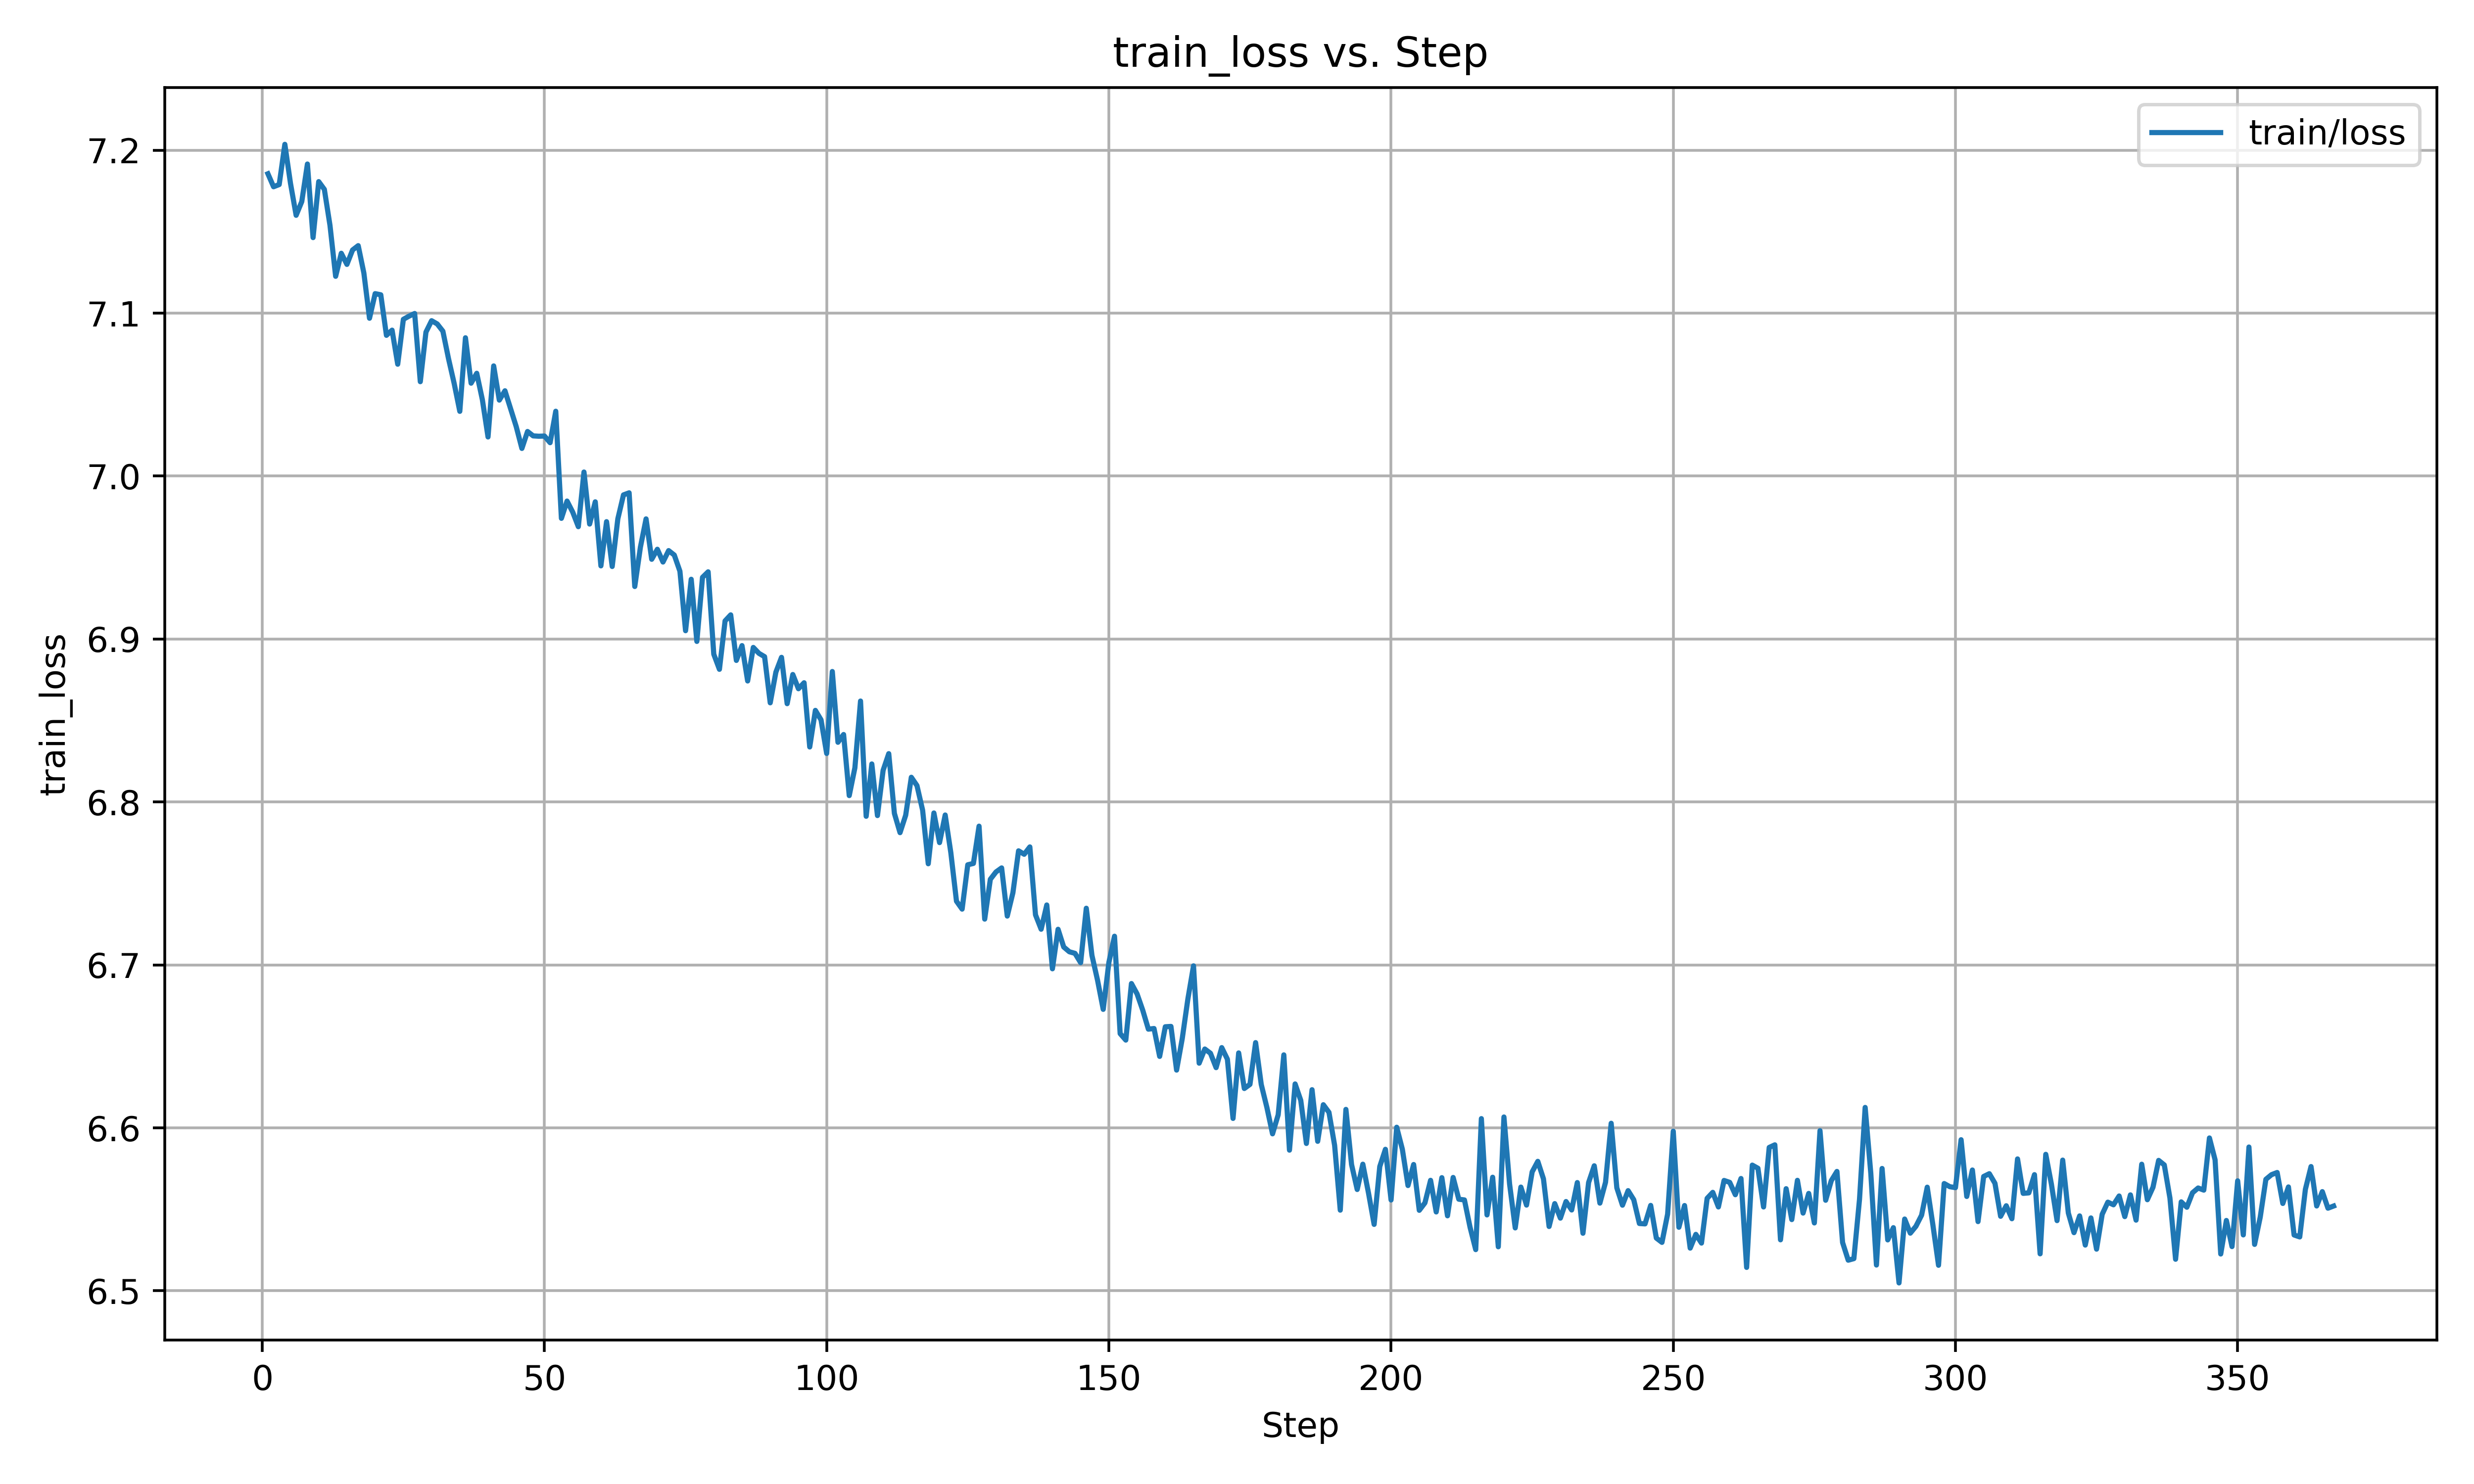
\includegraphics[width=\linewidth]{Transformer_train_loss.png}
		\caption{Training Loss}
		\label{fig:train_loss}
	\end{subfigure}
	\hfill
	\begin{subfigure}[b]{0.32\textwidth}
		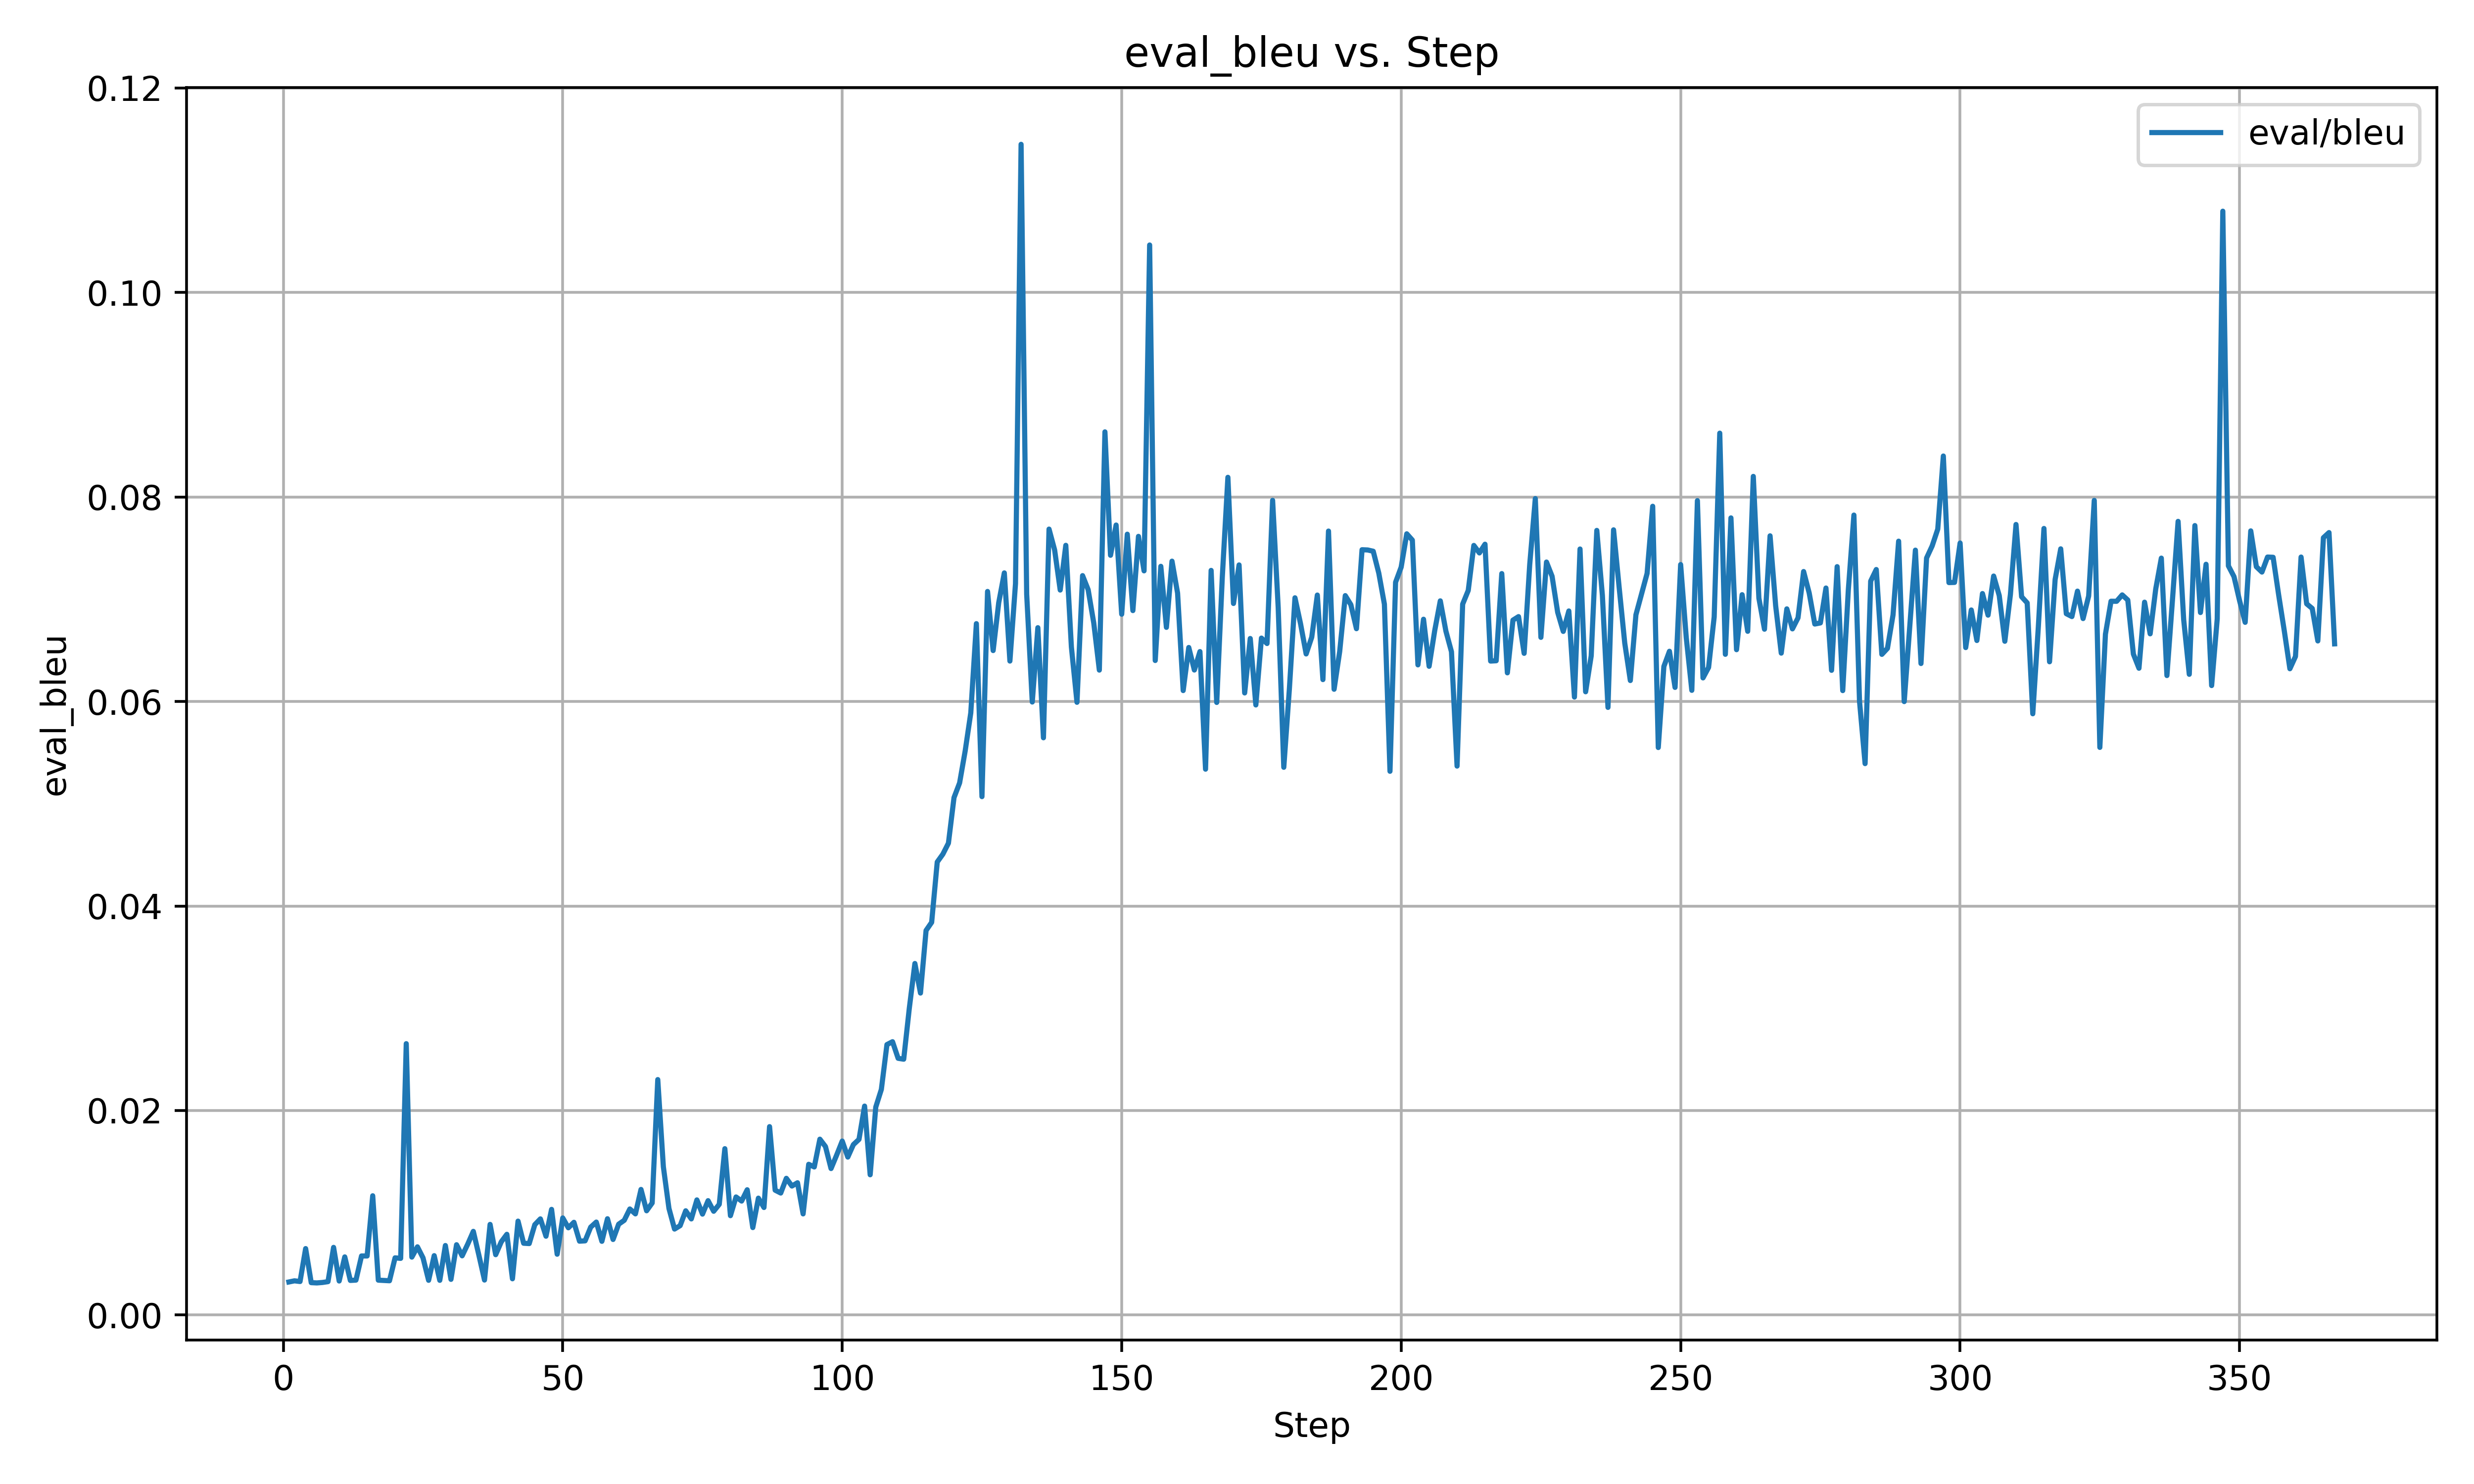
\includegraphics[width=\linewidth]{Transformer_eval_bleu.png}
		\caption{Evaluation BLEU}
		\label{fig:eval_bleu}
	\end{subfigure}
	\hfill
	\begin{subfigure}[b]{0.32\textwidth}
		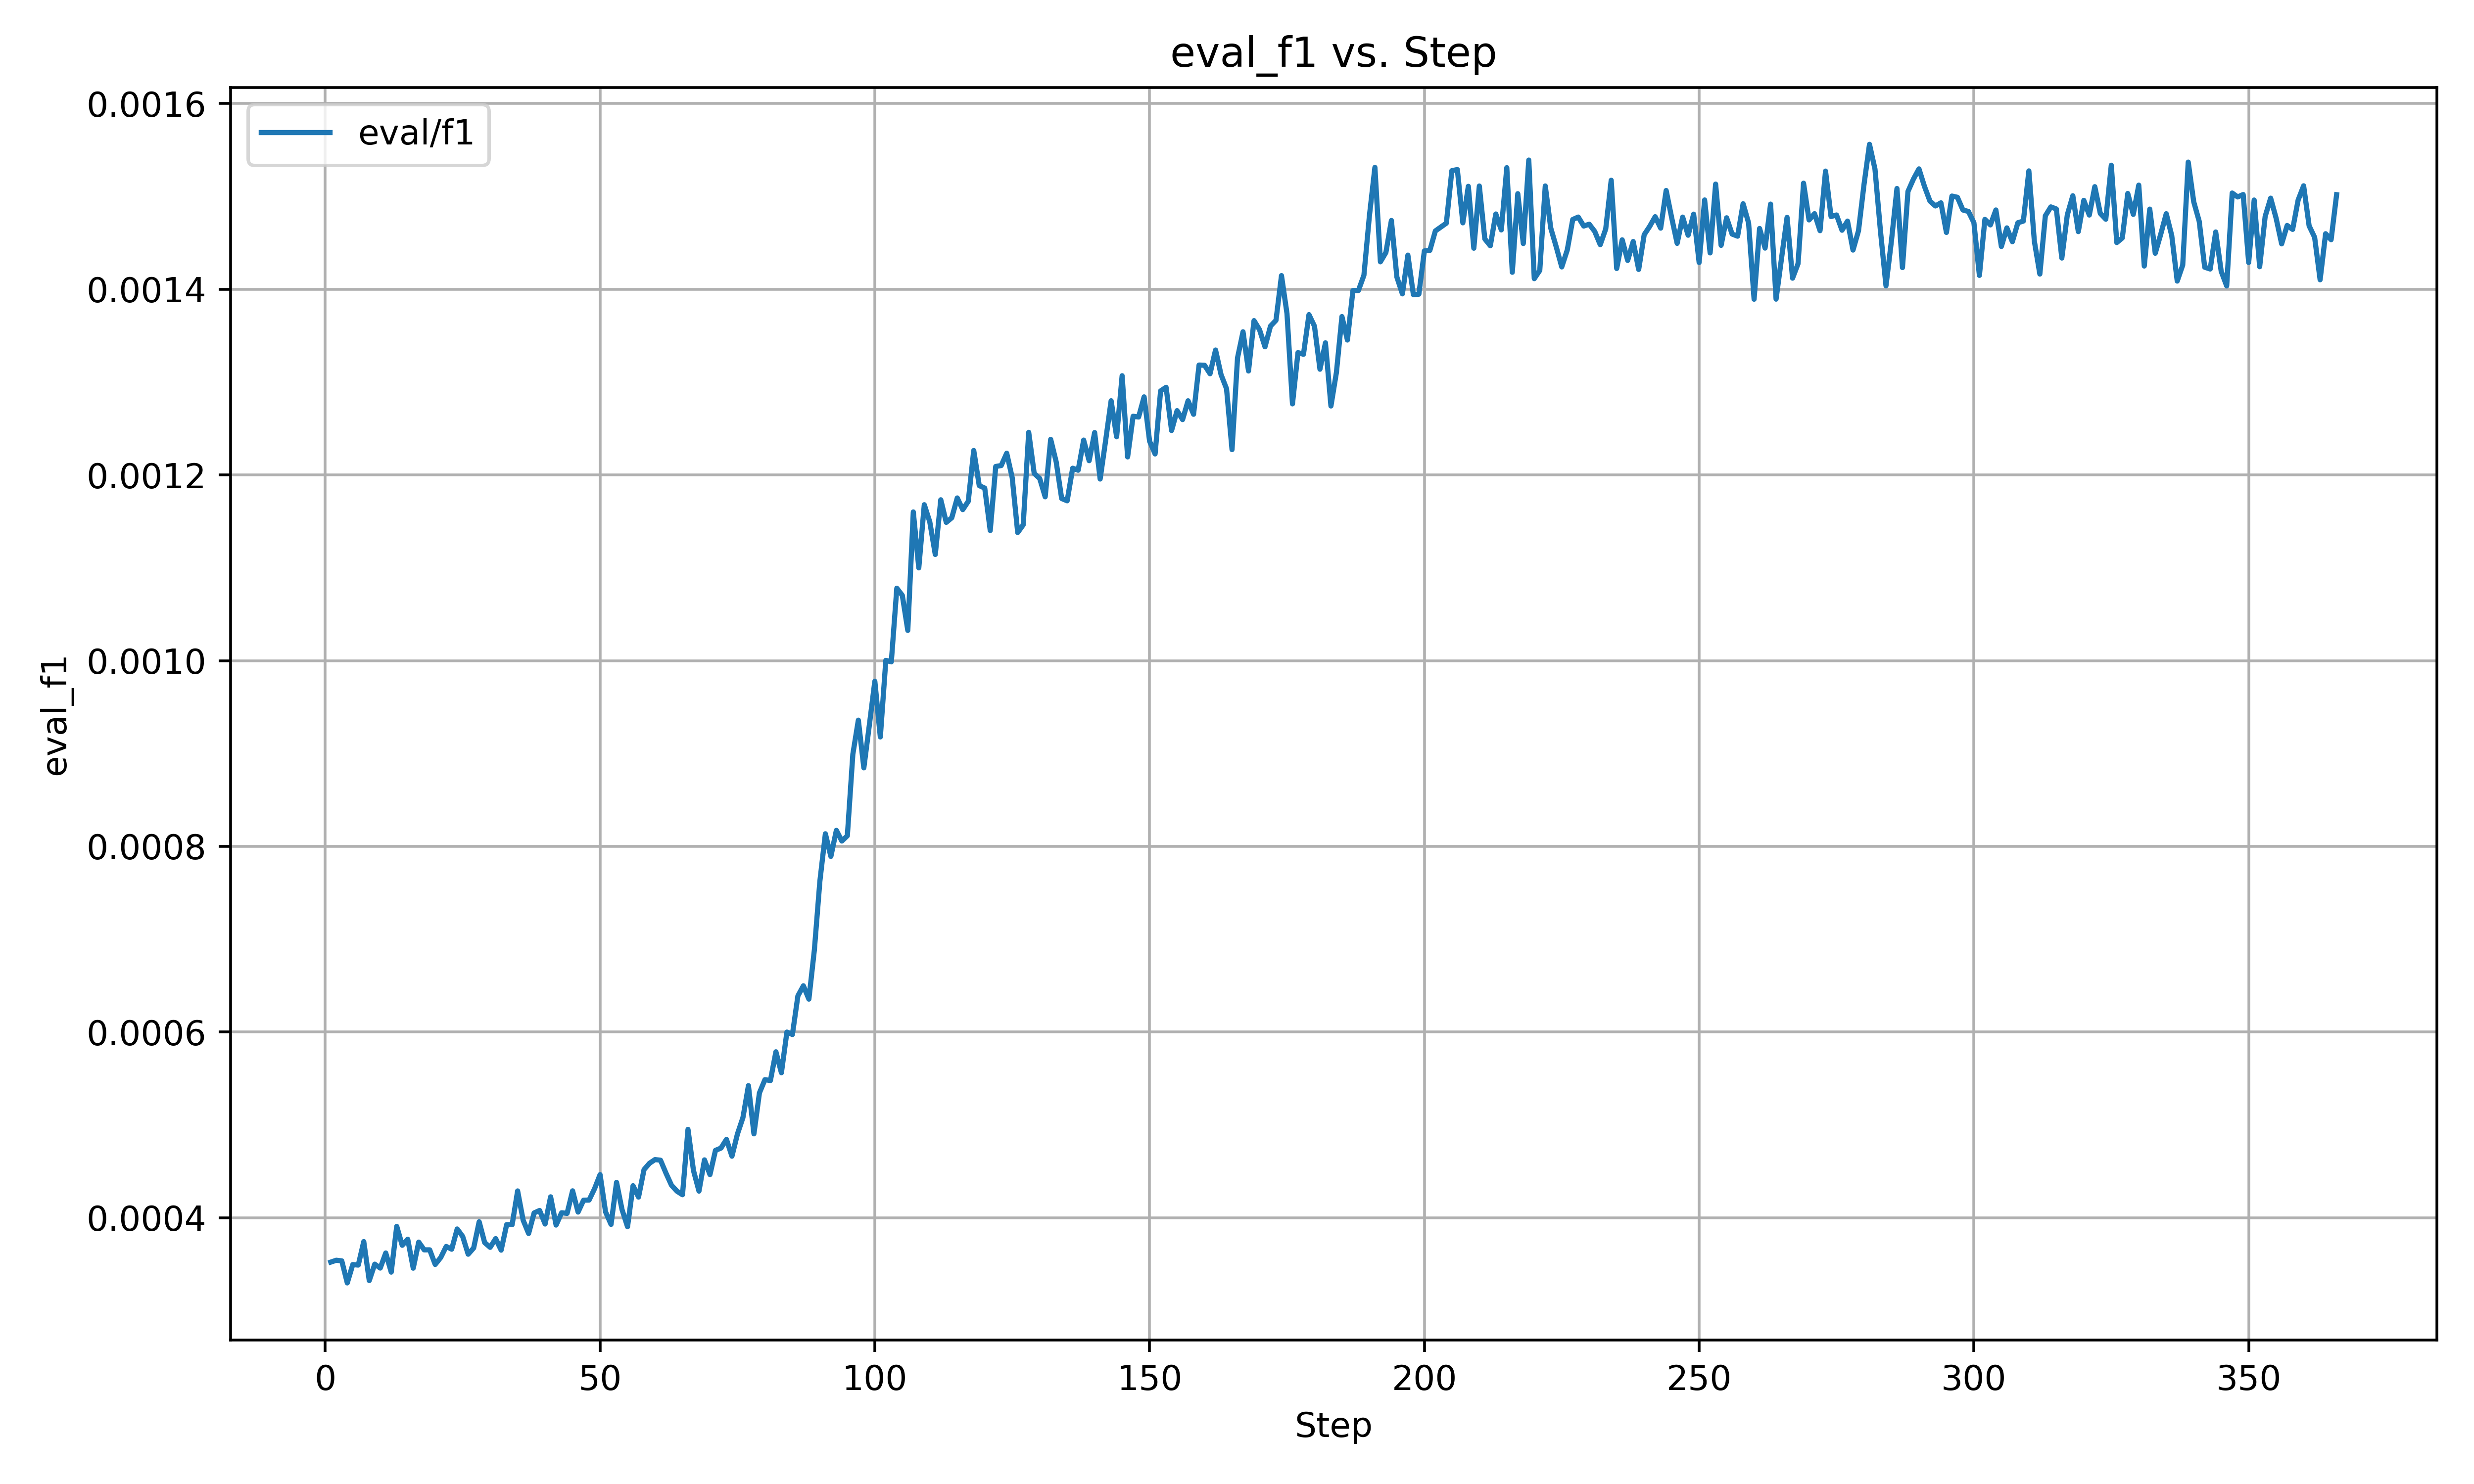
\includegraphics[width=\linewidth]{Transformer_eval_f1.png}
		\caption{Evaluation F1}
		\label{fig:eval_f1}
	\end{subfigure}
	\begin{subfigure}[b]{0.32\textwidth}
		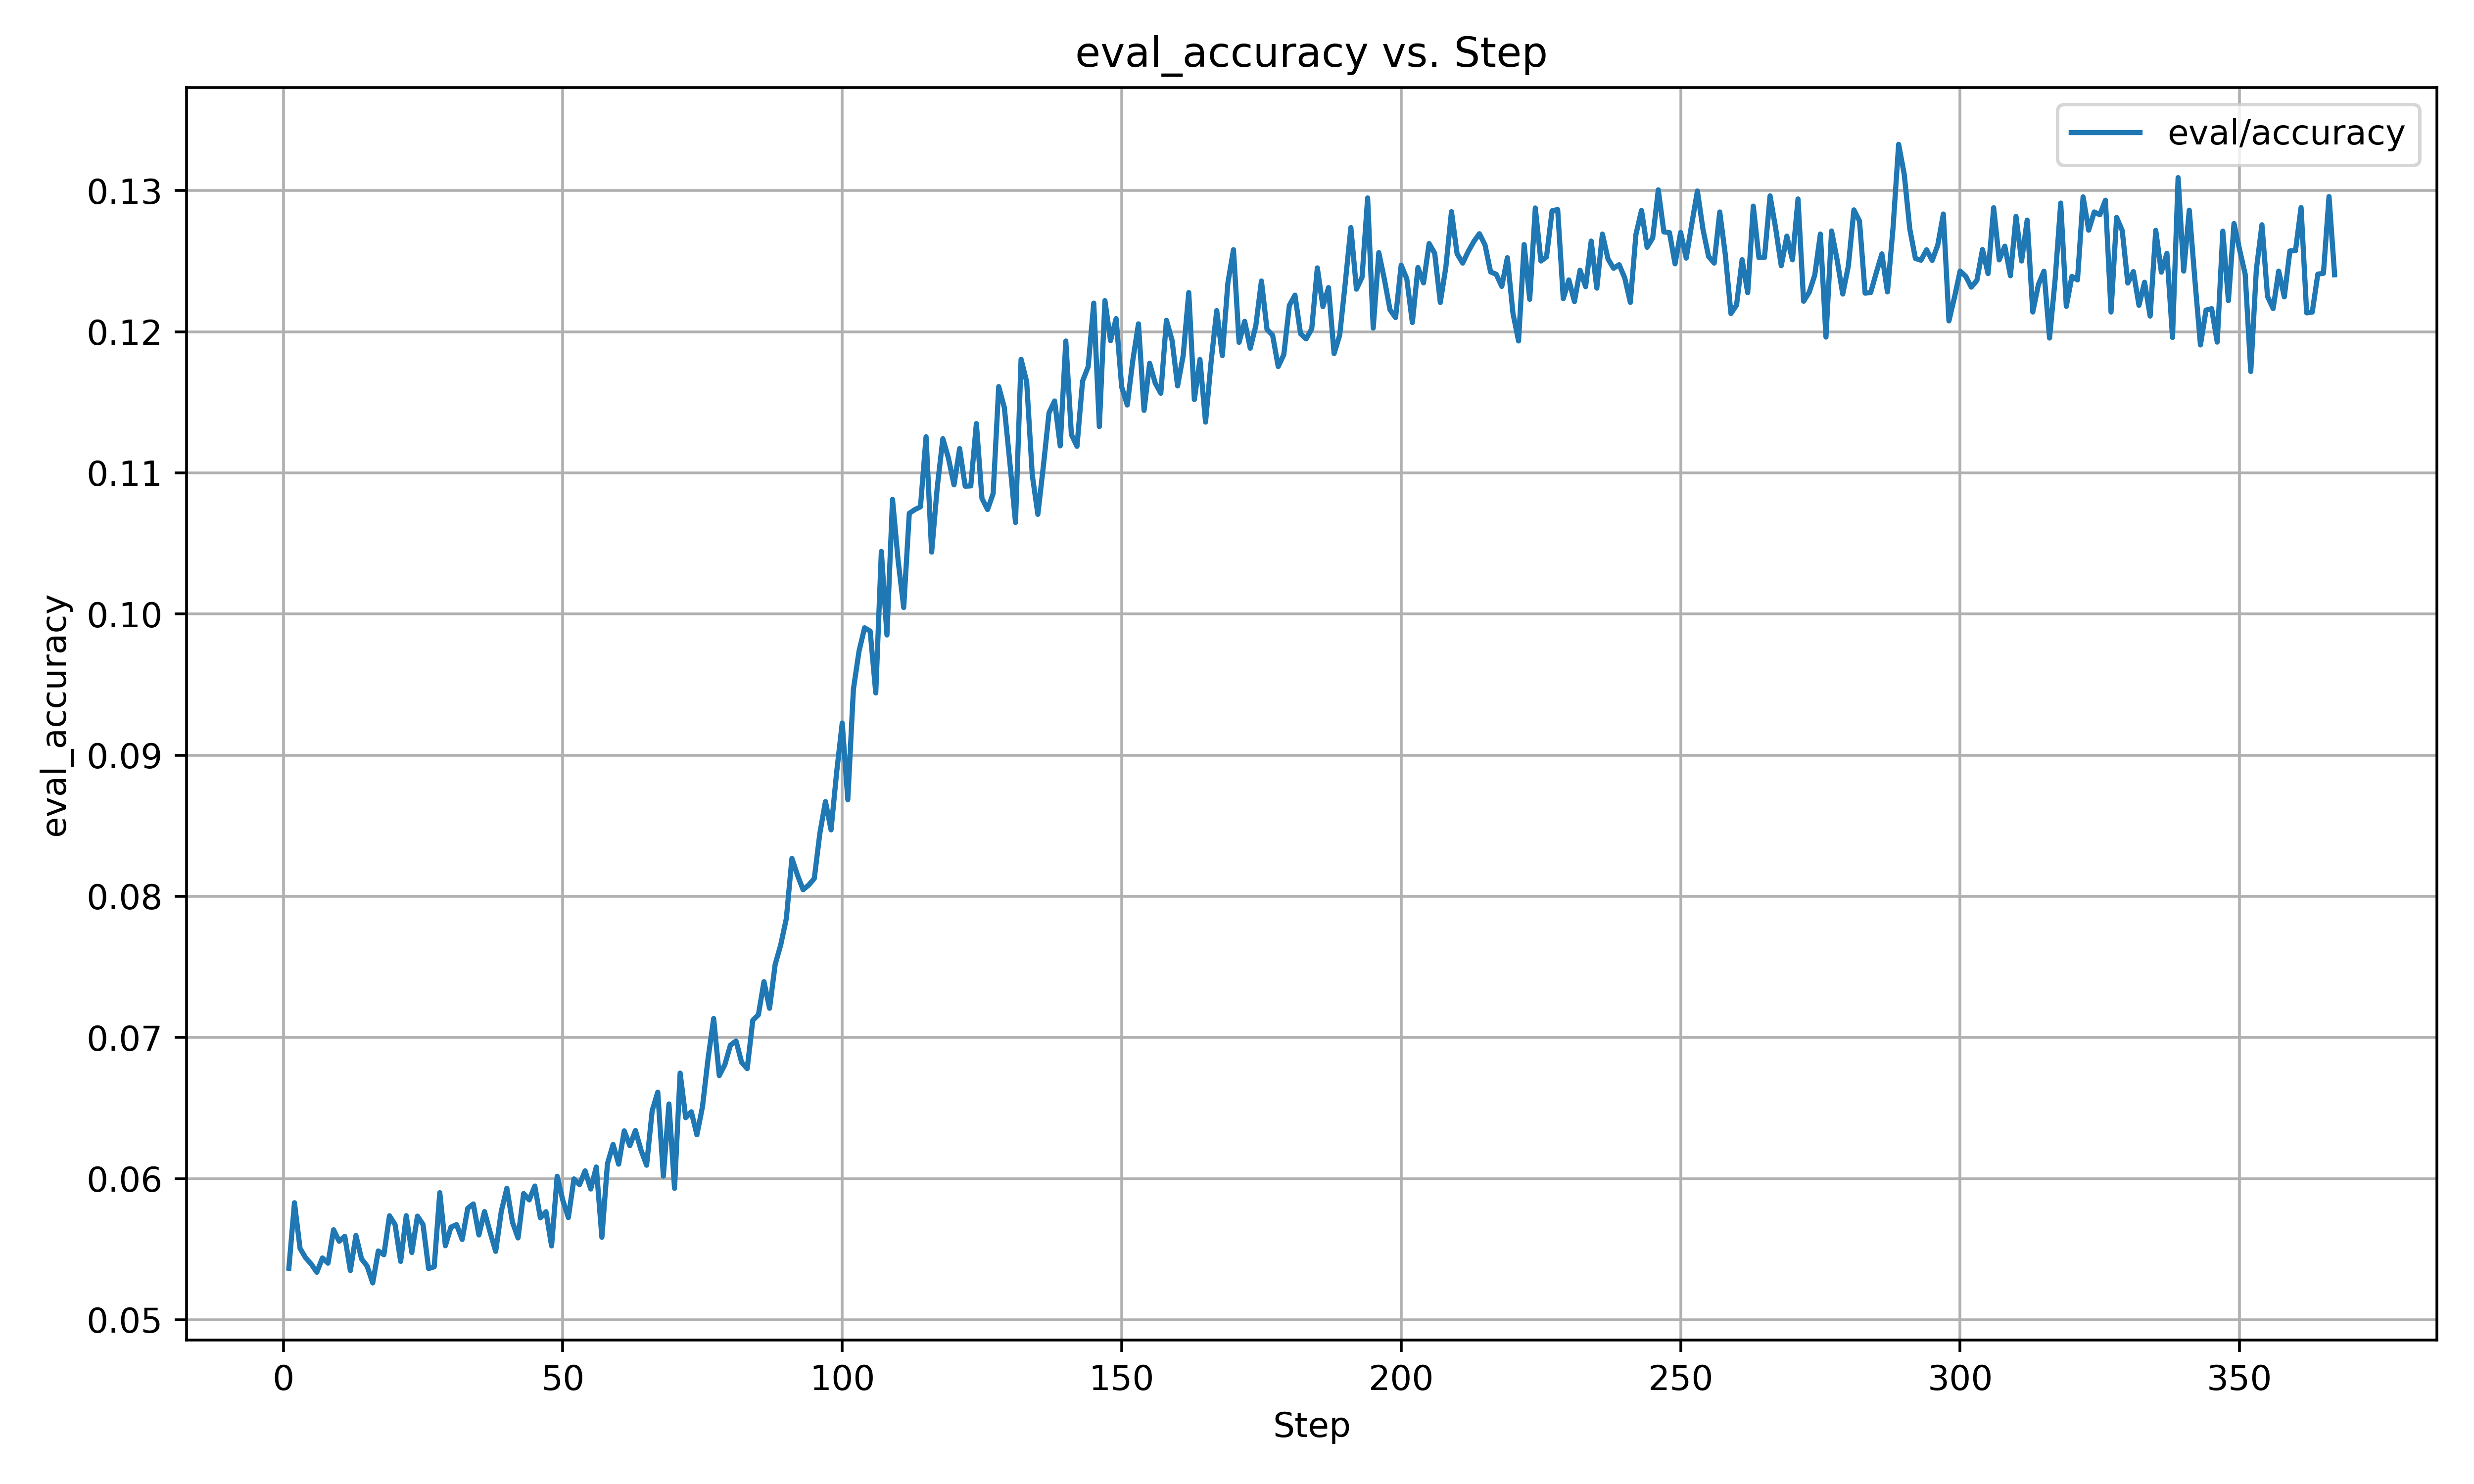
\includegraphics[width=\linewidth]{eval_accuracy.png}
		\caption{Evaluation Accuracy}
		\label{fig:eval_accuracy}
	\end{subfigure}
	\hfill
	\begin{subfigure}[b]{0.32\textwidth}
		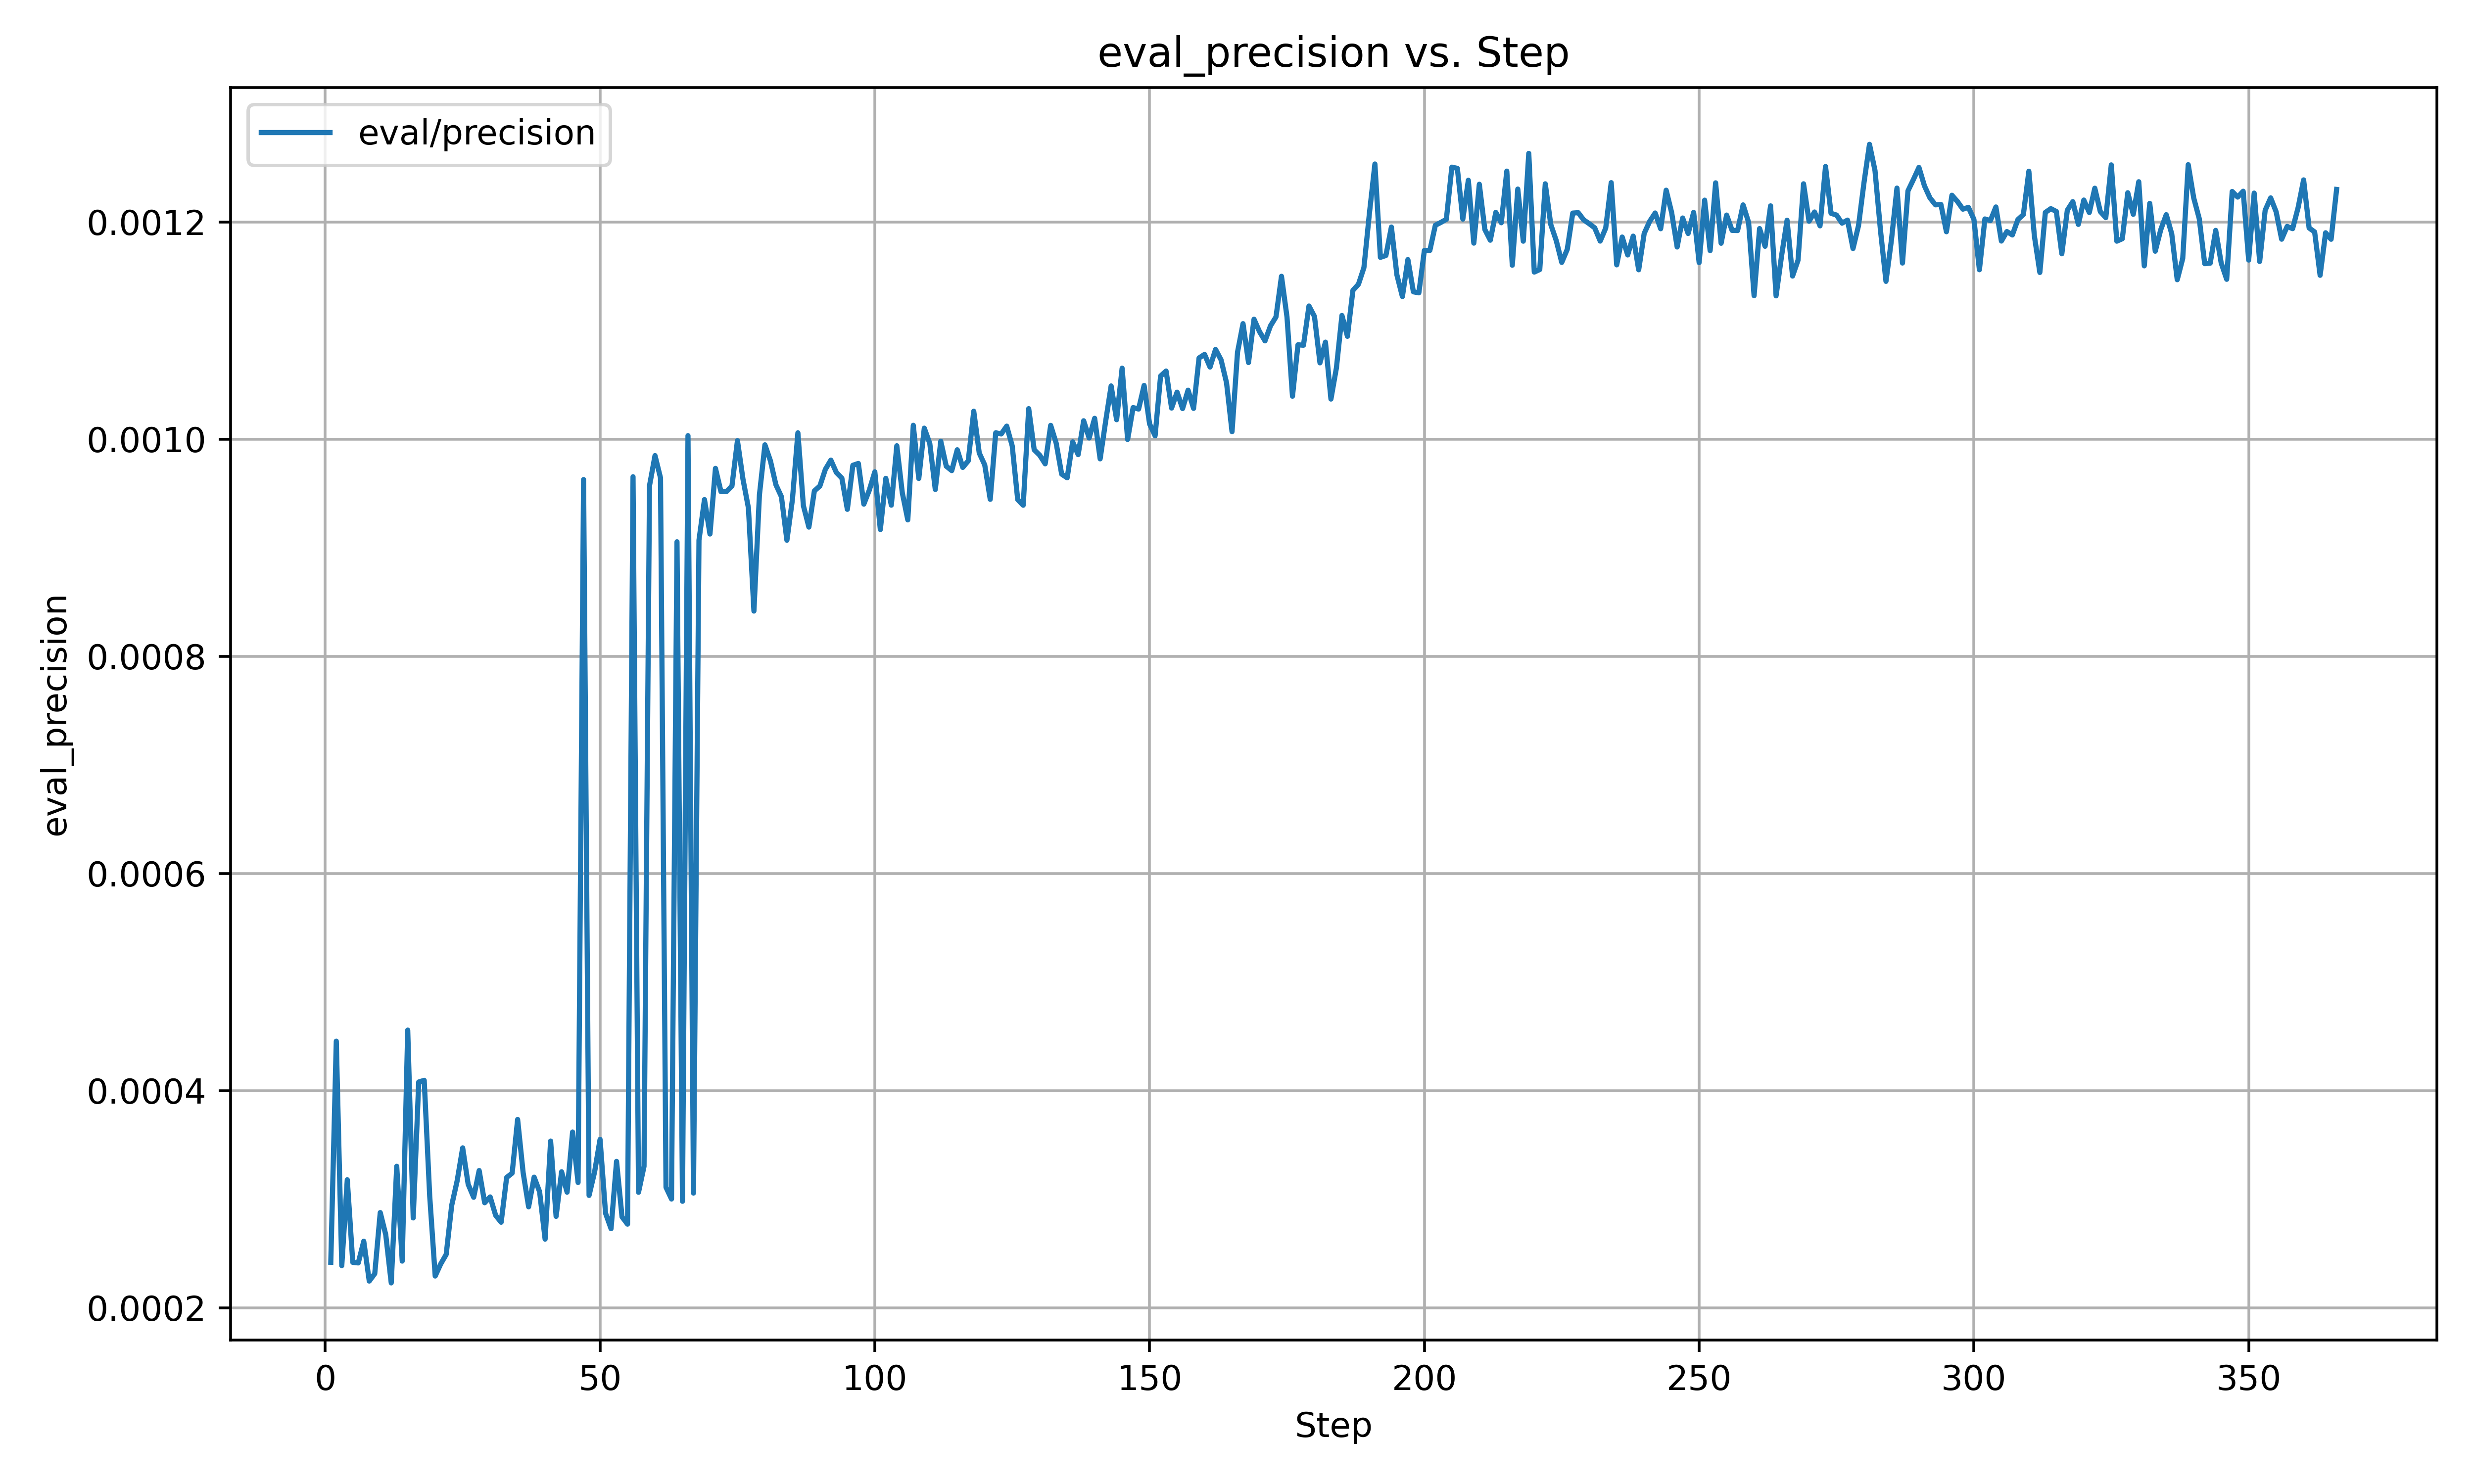
\includegraphics[width=\linewidth]{eval_precision.png}
		\caption{Precision Curve}
		\label{fig:eval_precision}
	\end{subfigure}
	\hfill
	\begin{subfigure}[b]{0.32\textwidth}
		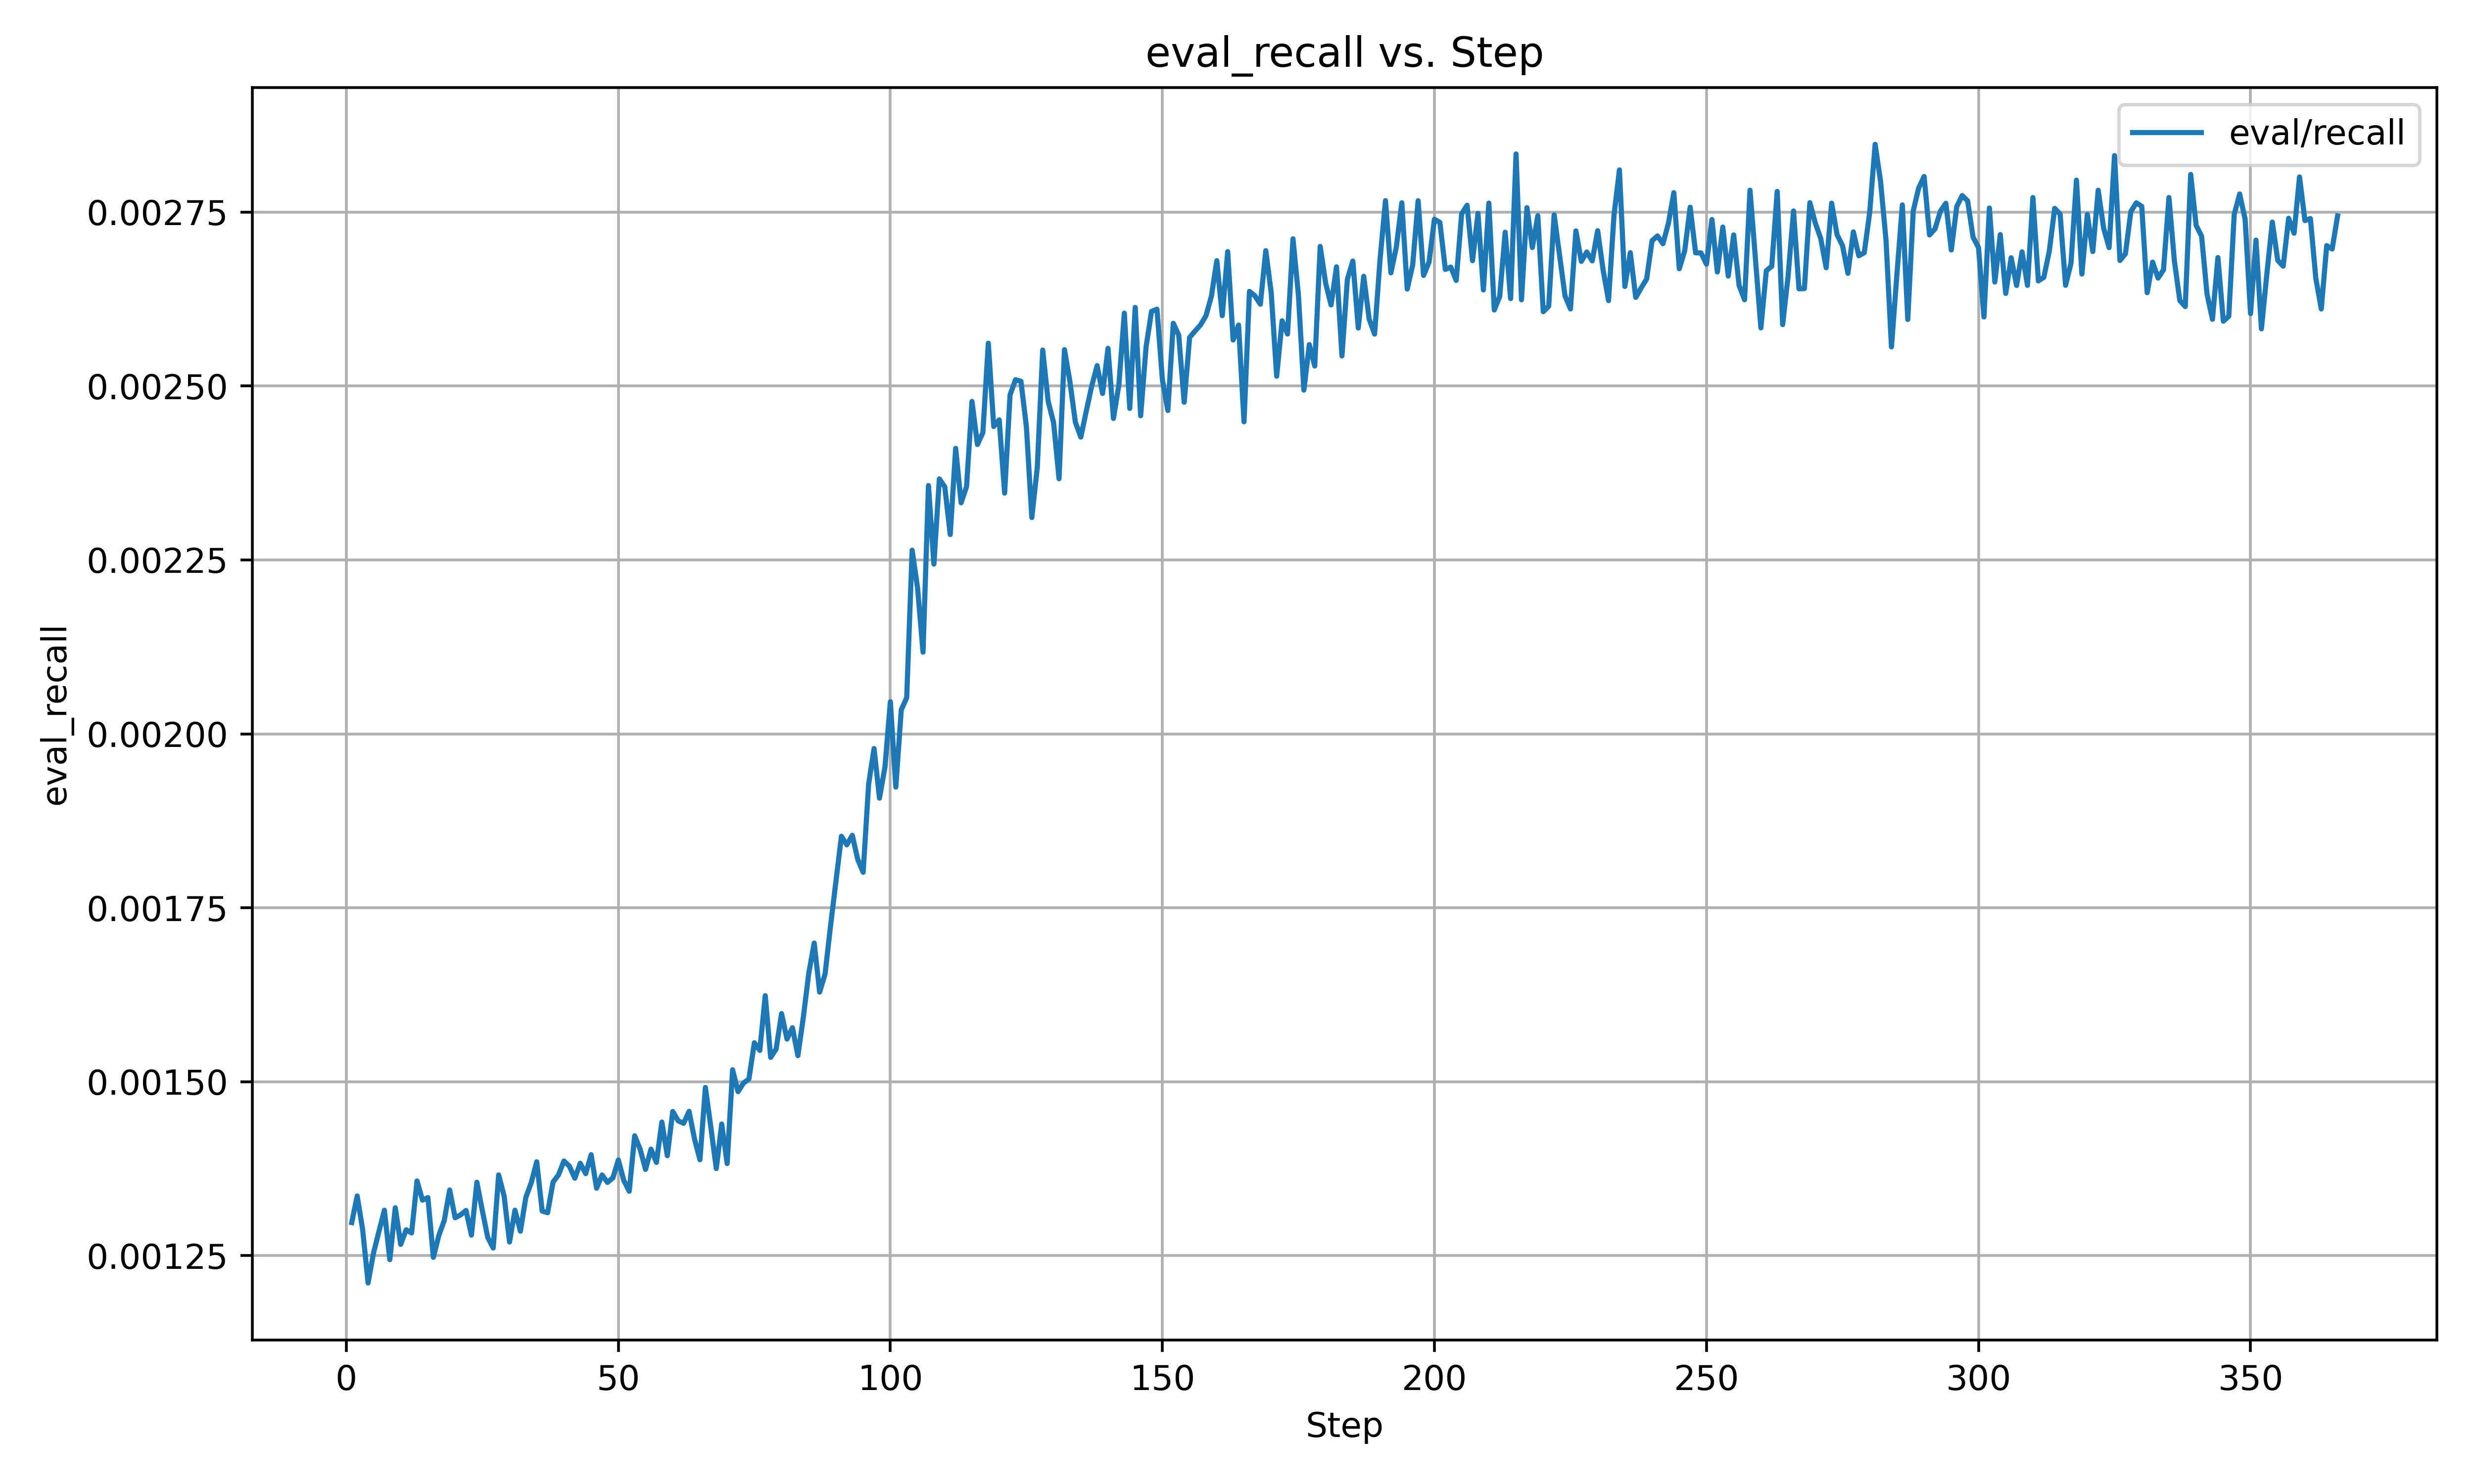
\includegraphics[width=\linewidth]{eval_recall.png}
		\caption{Recall Curve}
		\label{fig:eval_recall}
	\end{subfigure}
	\caption{Performance metrics of the TNMT model.}
	\label{fig:tnmt_performance}
\end{figure}

Next, we evaluated a fine-tuned Chinese BERT model. Figures~\ref{fig:bert_training_performance} show the training accuracy, F1 score, loss, learning rate, precision, and recall over epochs. The model exhibits a steady increase in accuracy and F1 score, with a corresponding decrease in loss. Precision and recall curves also show consistent improvement, indicating the model's ability to capture nuanced sentiment cues in the translated texts. However, overall this model perform bad in the financial sentiment analysis task. This may due to the translation quality and the lexicon-based annotation.

\begin{figure}[!ht]
	\centering
	\begin{subfigure}[b]{0.32\textwidth}
		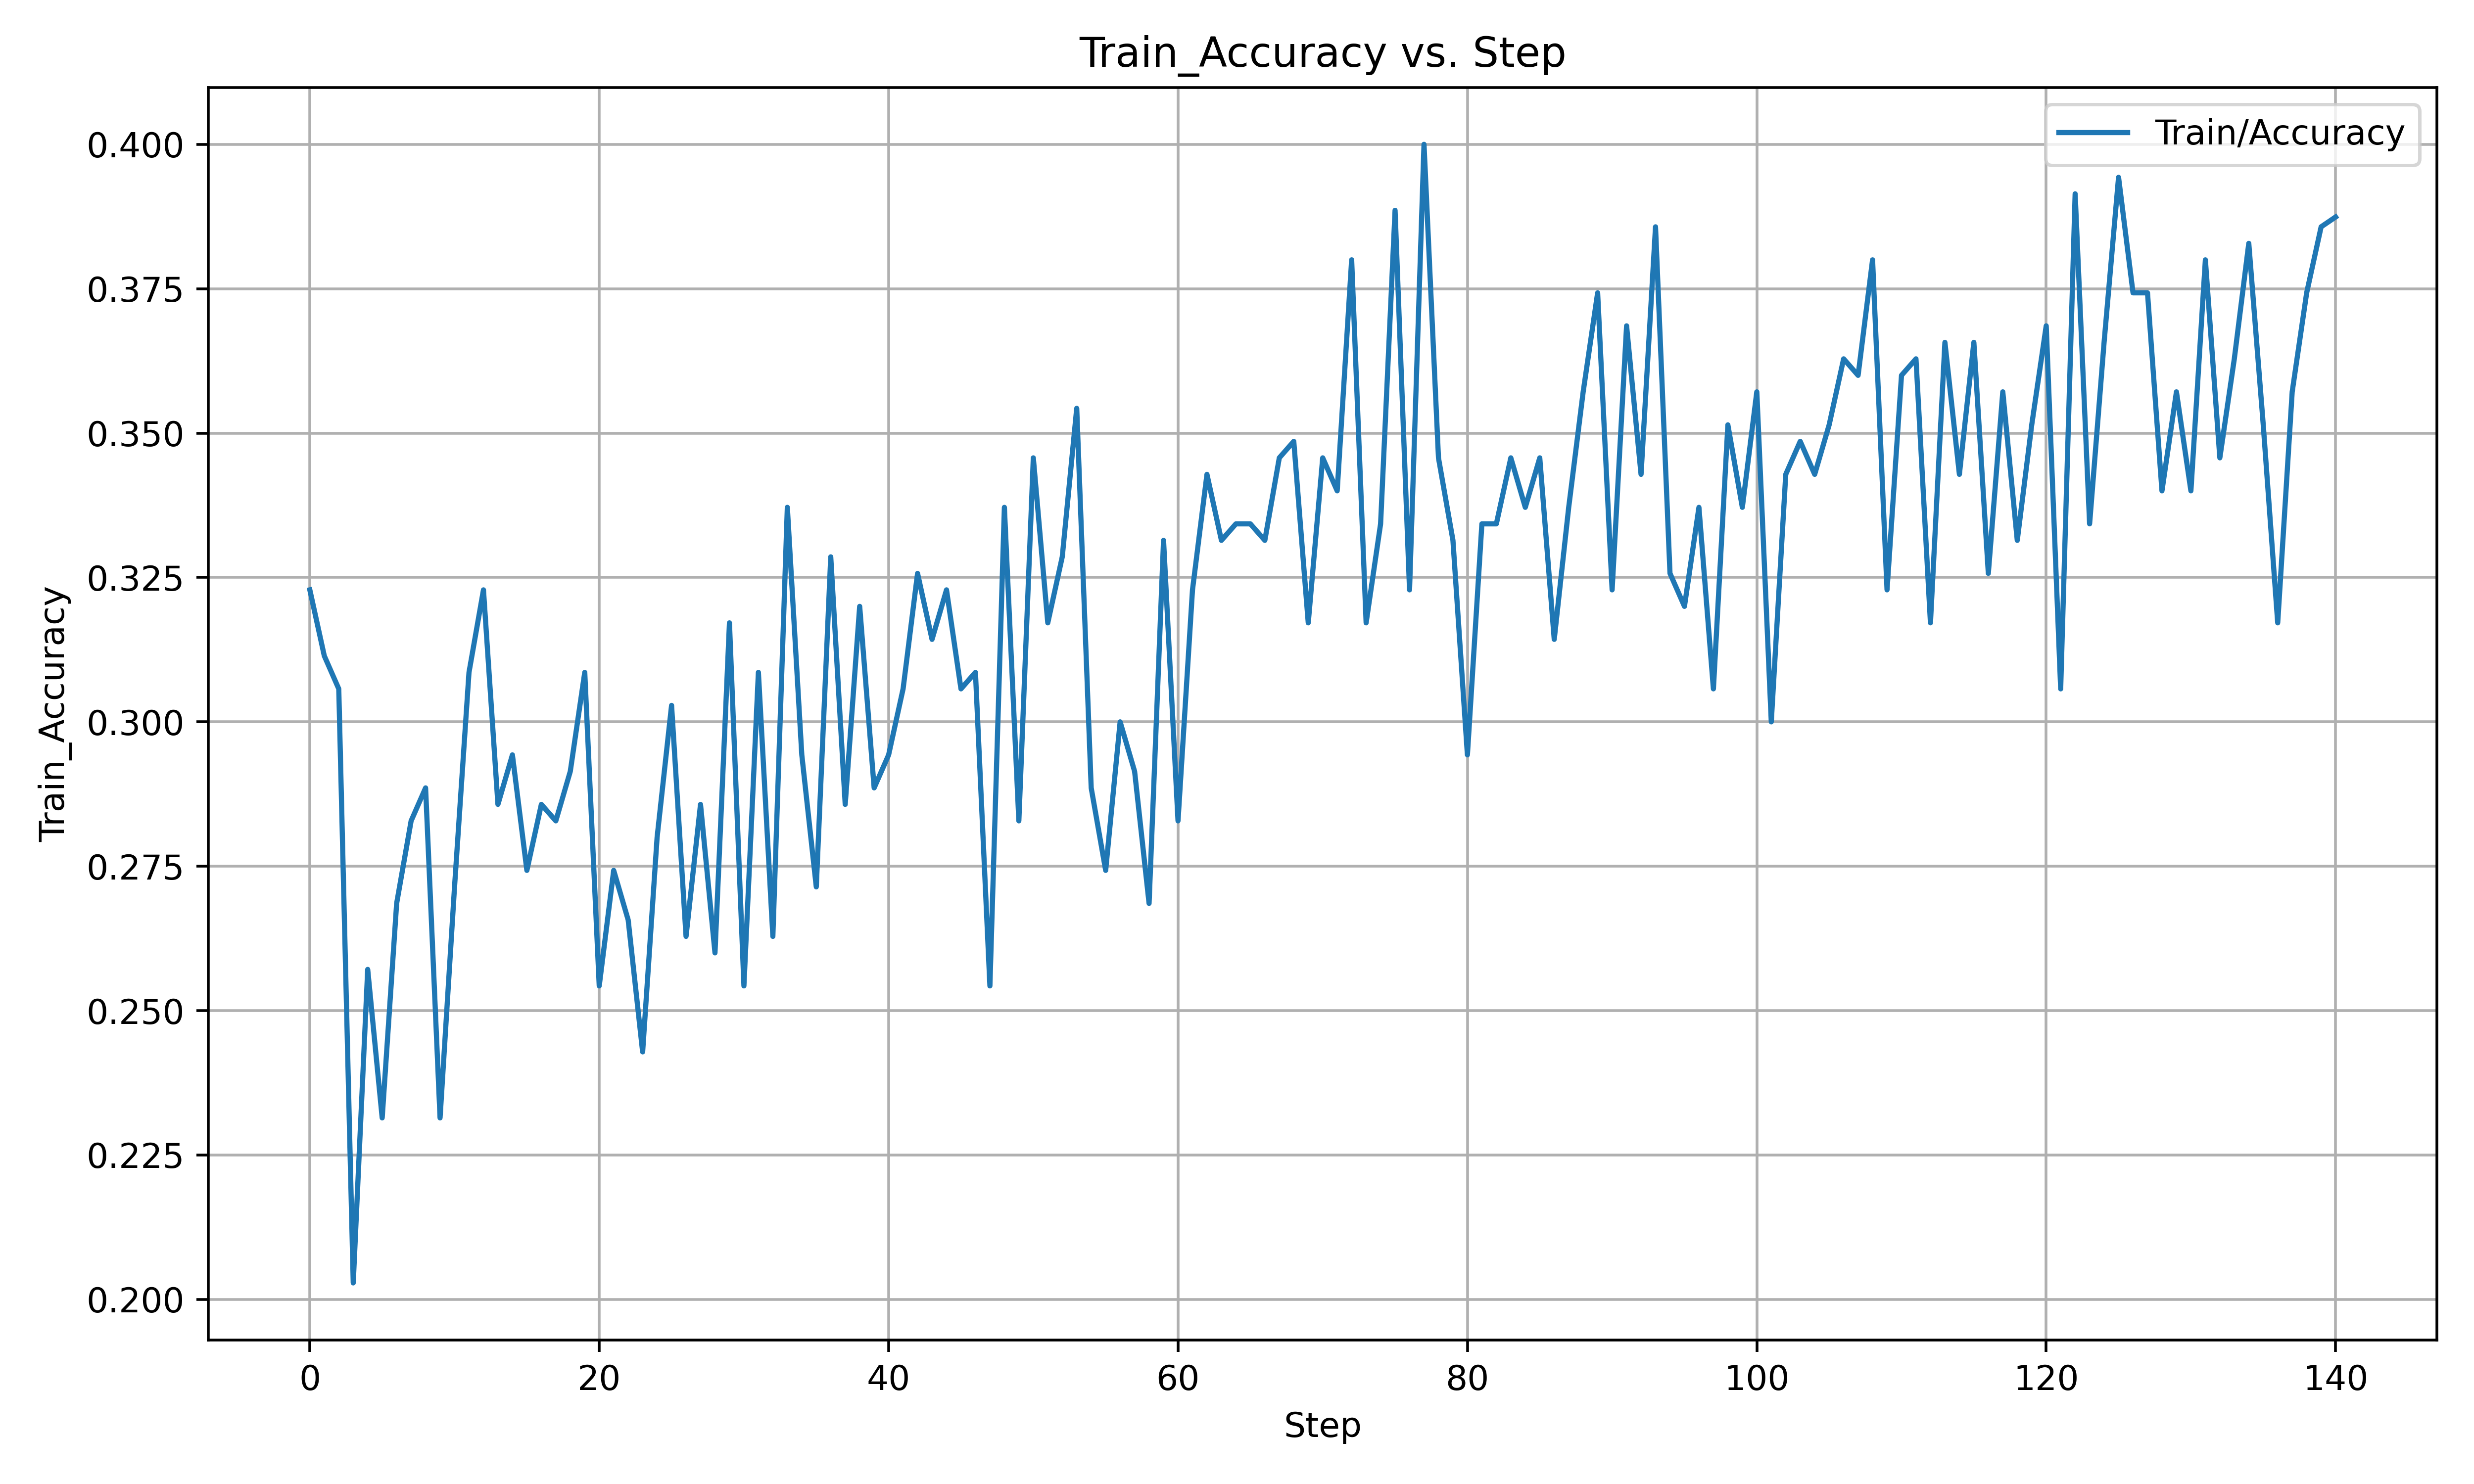
\includegraphics[width=\linewidth]{BERT_Train_Accuracy.png}
		\caption{Training Accuracy}
	\end{subfigure}
	\hfill
	\begin{subfigure}[b]{0.32\textwidth}
		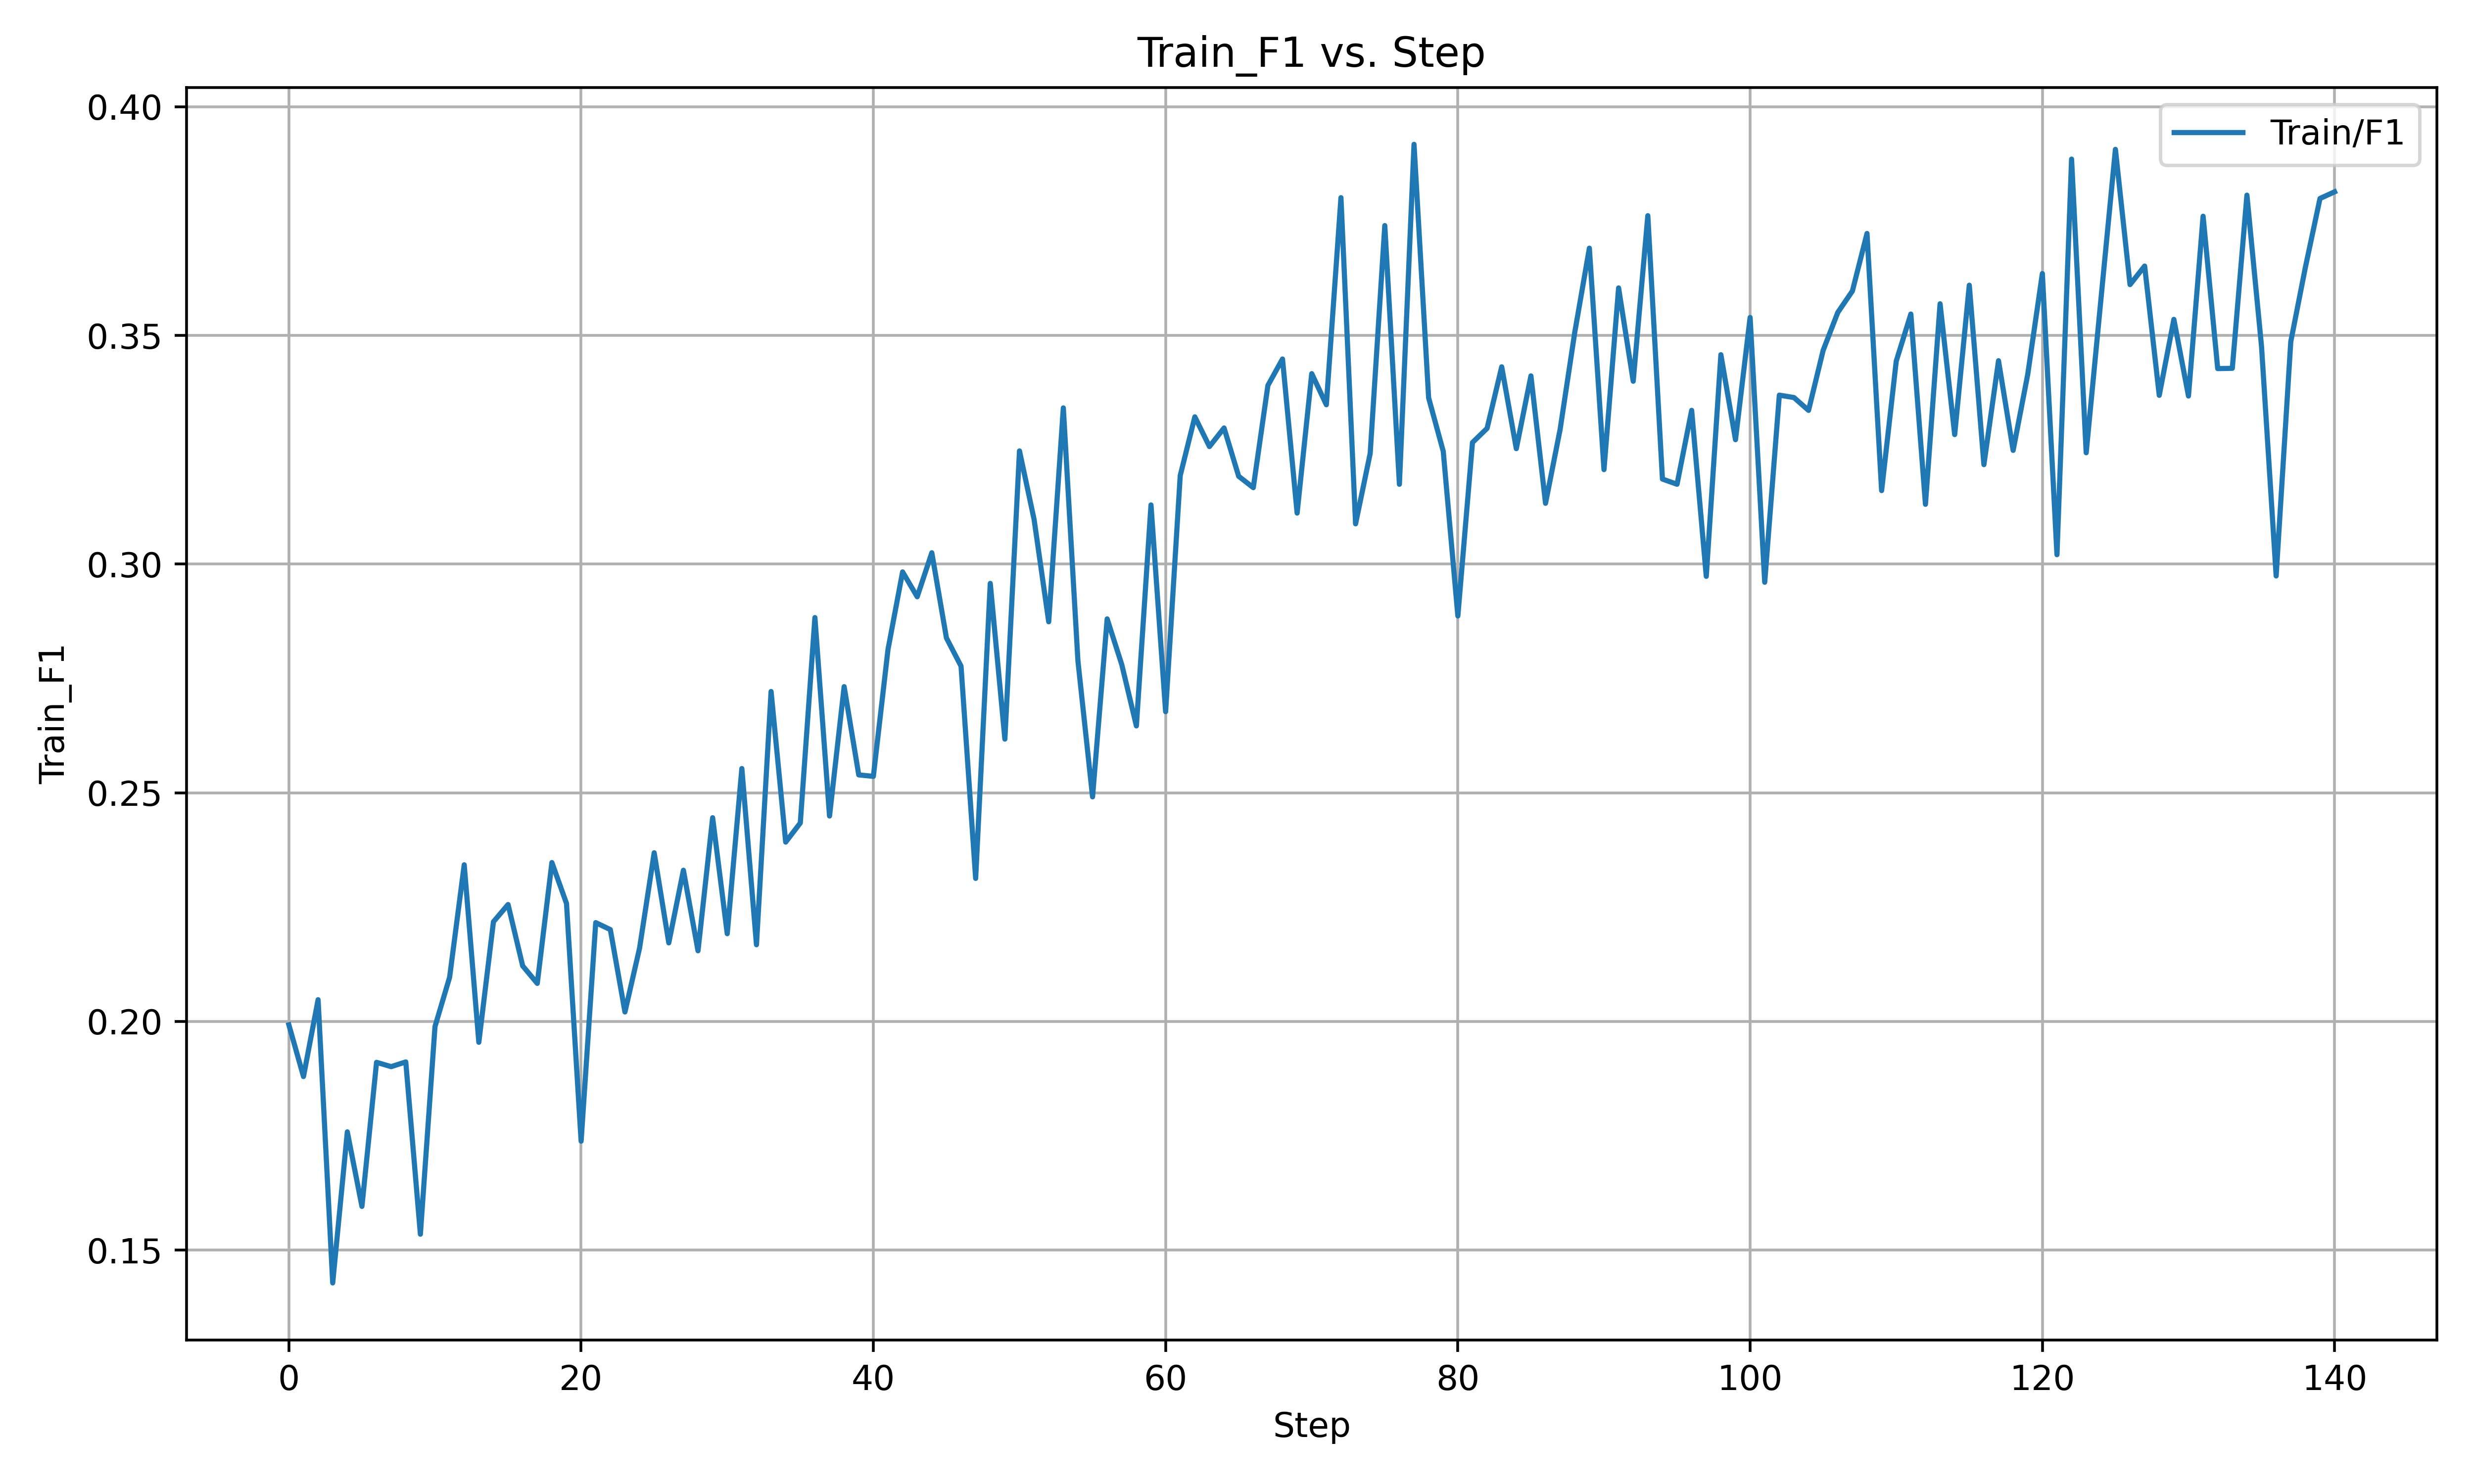
\includegraphics[width=\linewidth]{BERT_Train_F1.png}
		\caption{Training F1 Score}
	\end{subfigure}
	\hfill
	\begin{subfigure}[b]{0.32\textwidth}
		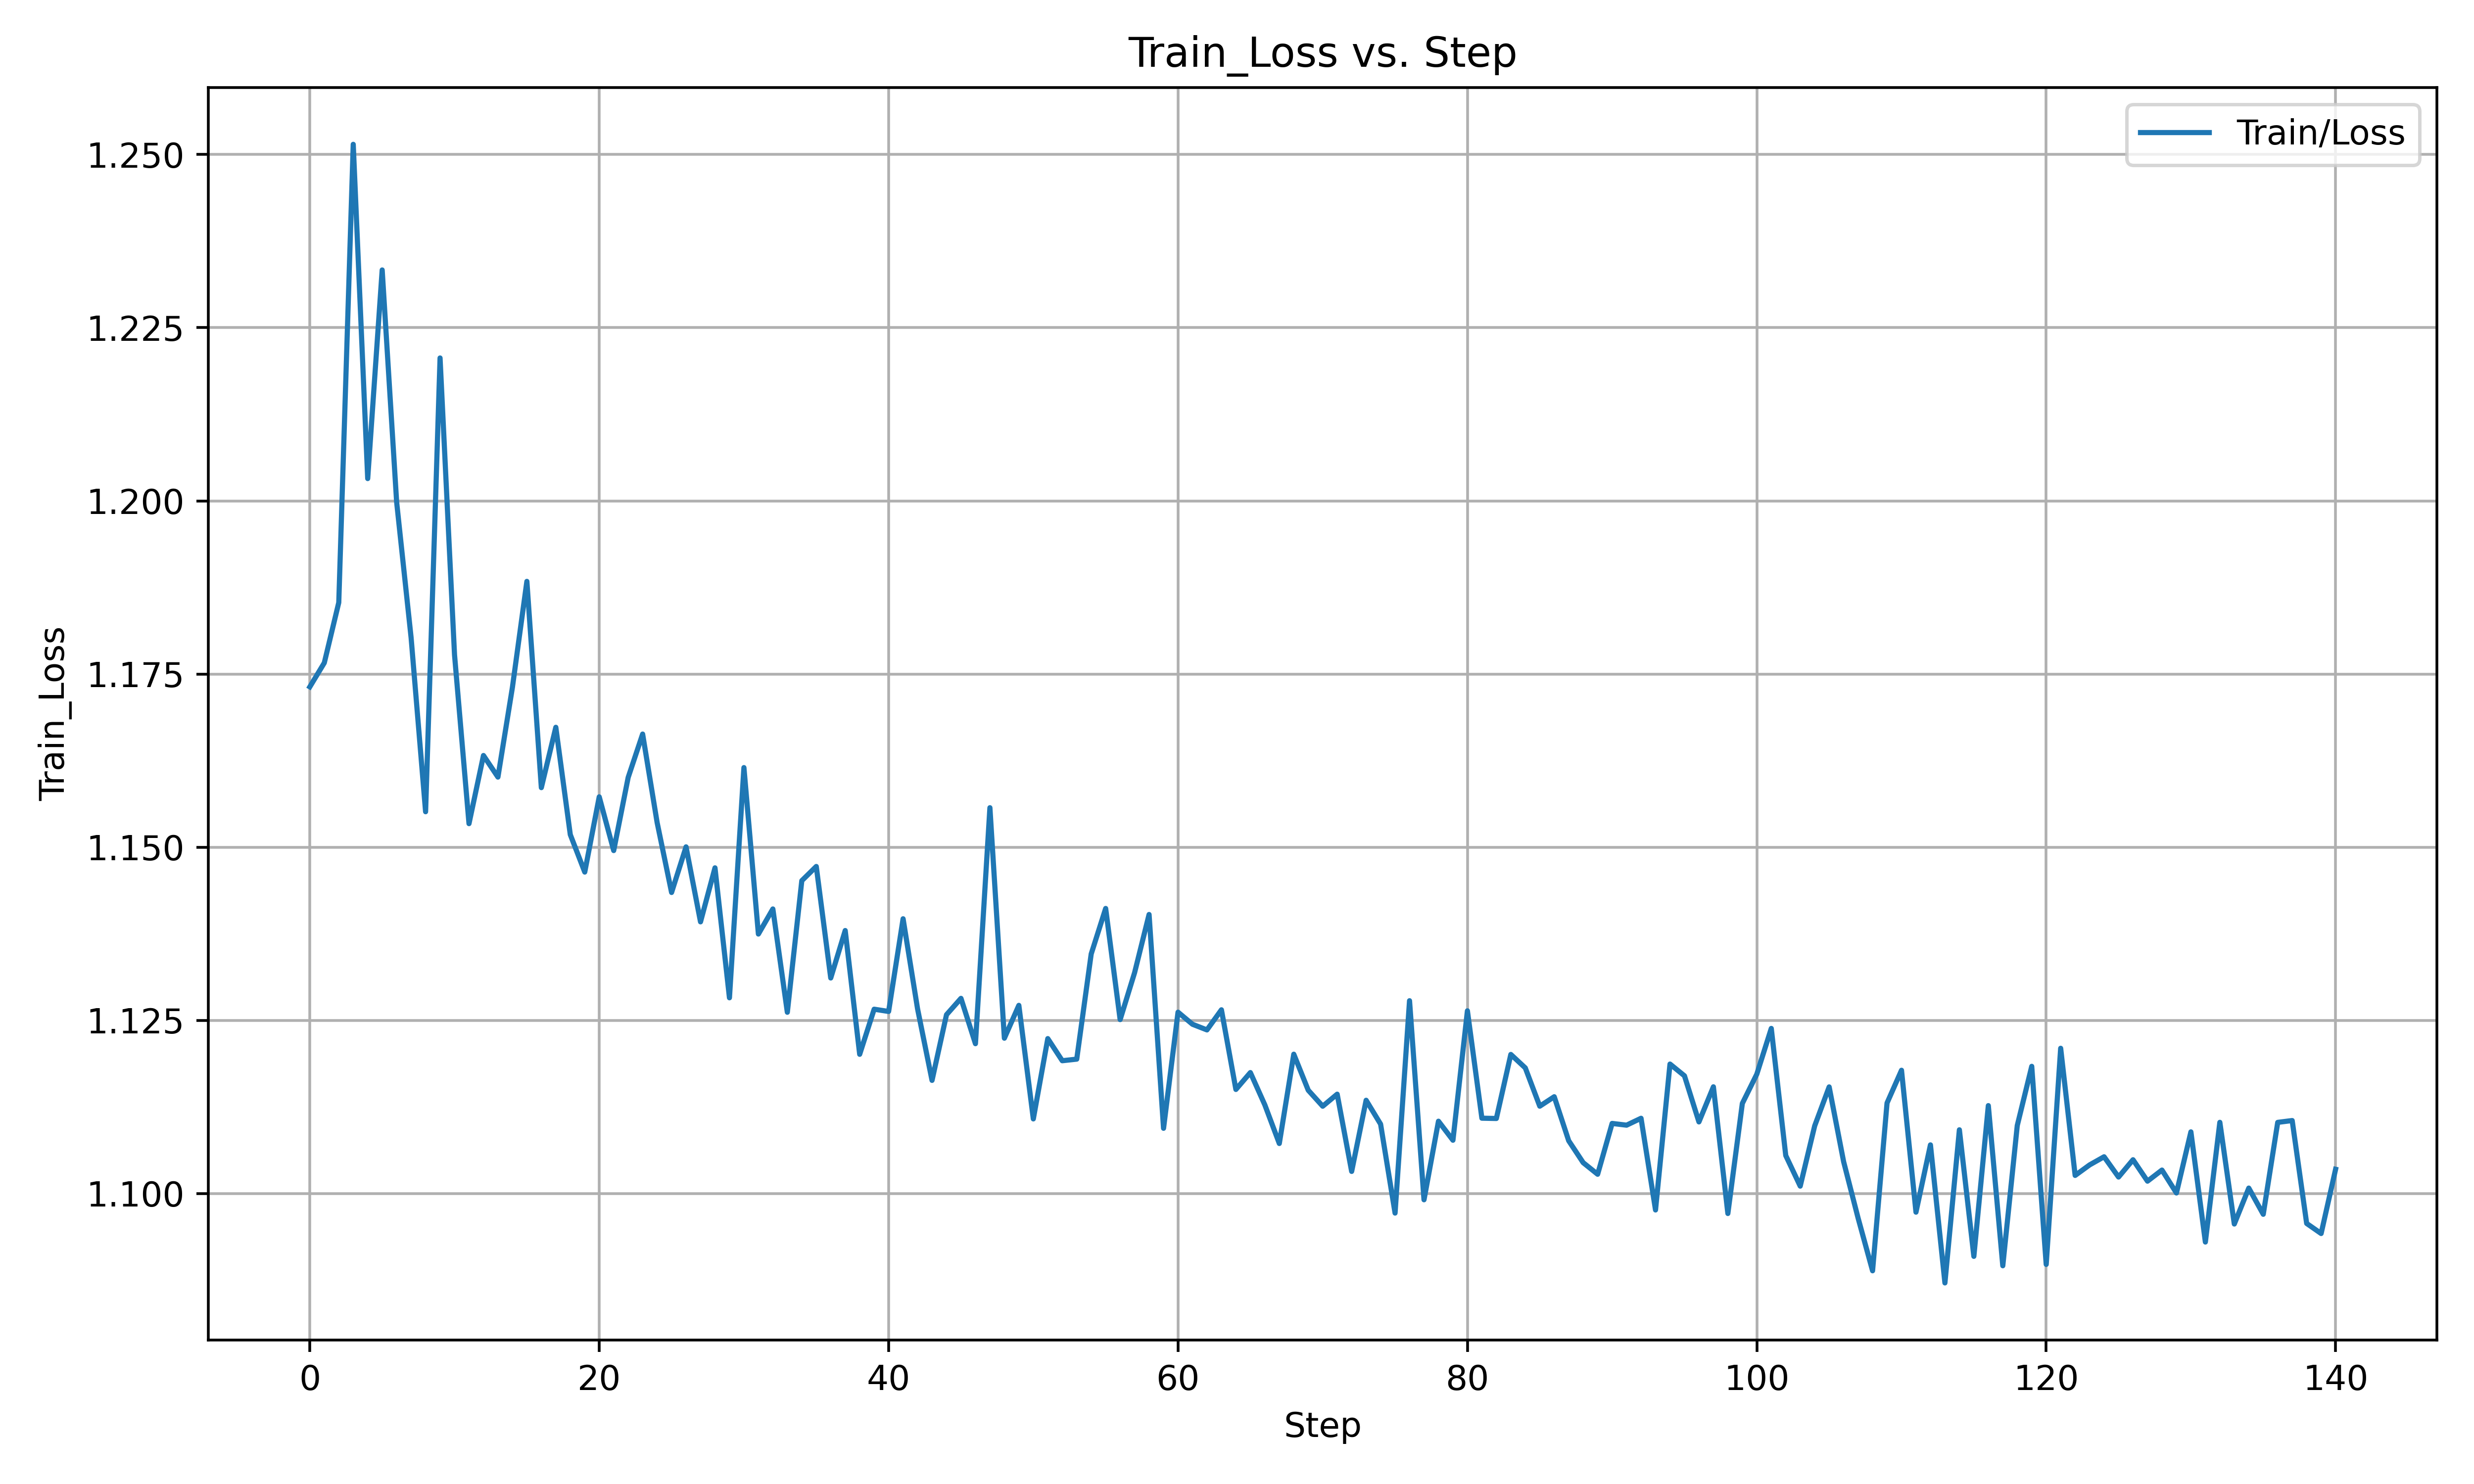
\includegraphics[width=\linewidth]{BERT_Train_Loss.png}
		\caption{Training Loss}
	\end{subfigure}
	
	\begin{subfigure}[b]{0.32\textwidth}
		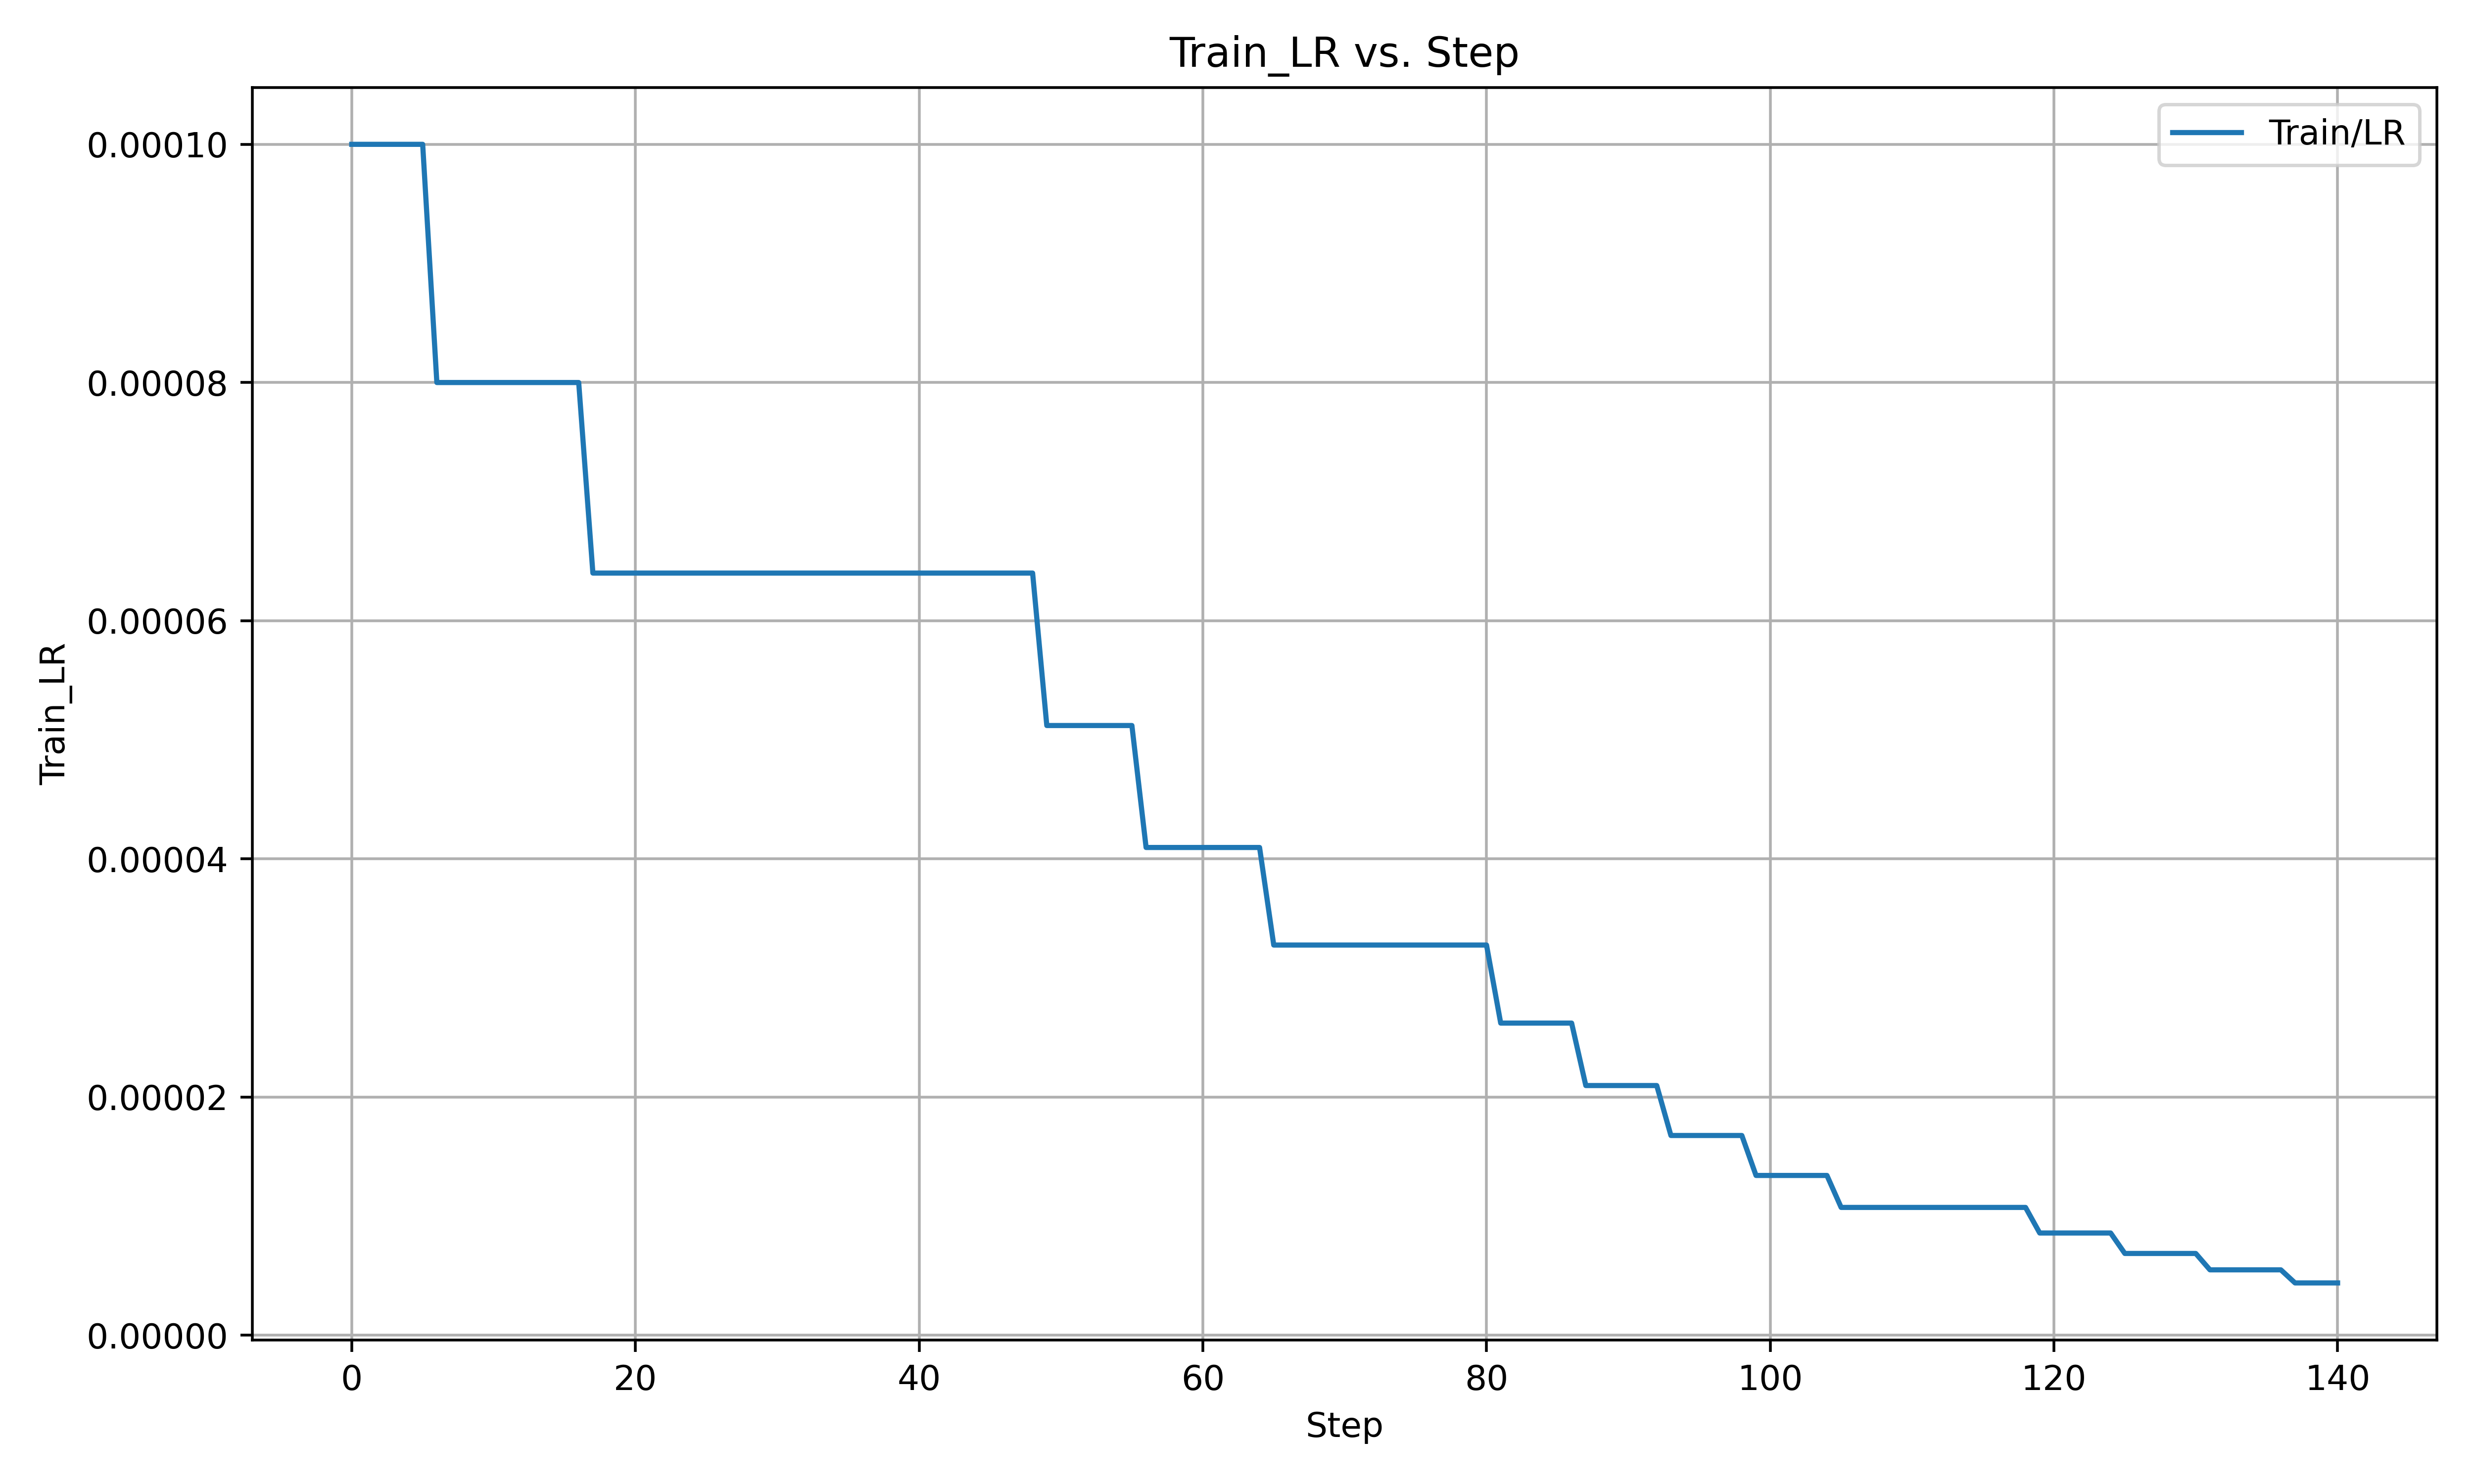
\includegraphics[width=\linewidth]{Train_LR.png}
		\caption{Training Learning Rate}
	\end{subfigure}
	\hfill
	\begin{subfigure}[b]{0.32\textwidth}
		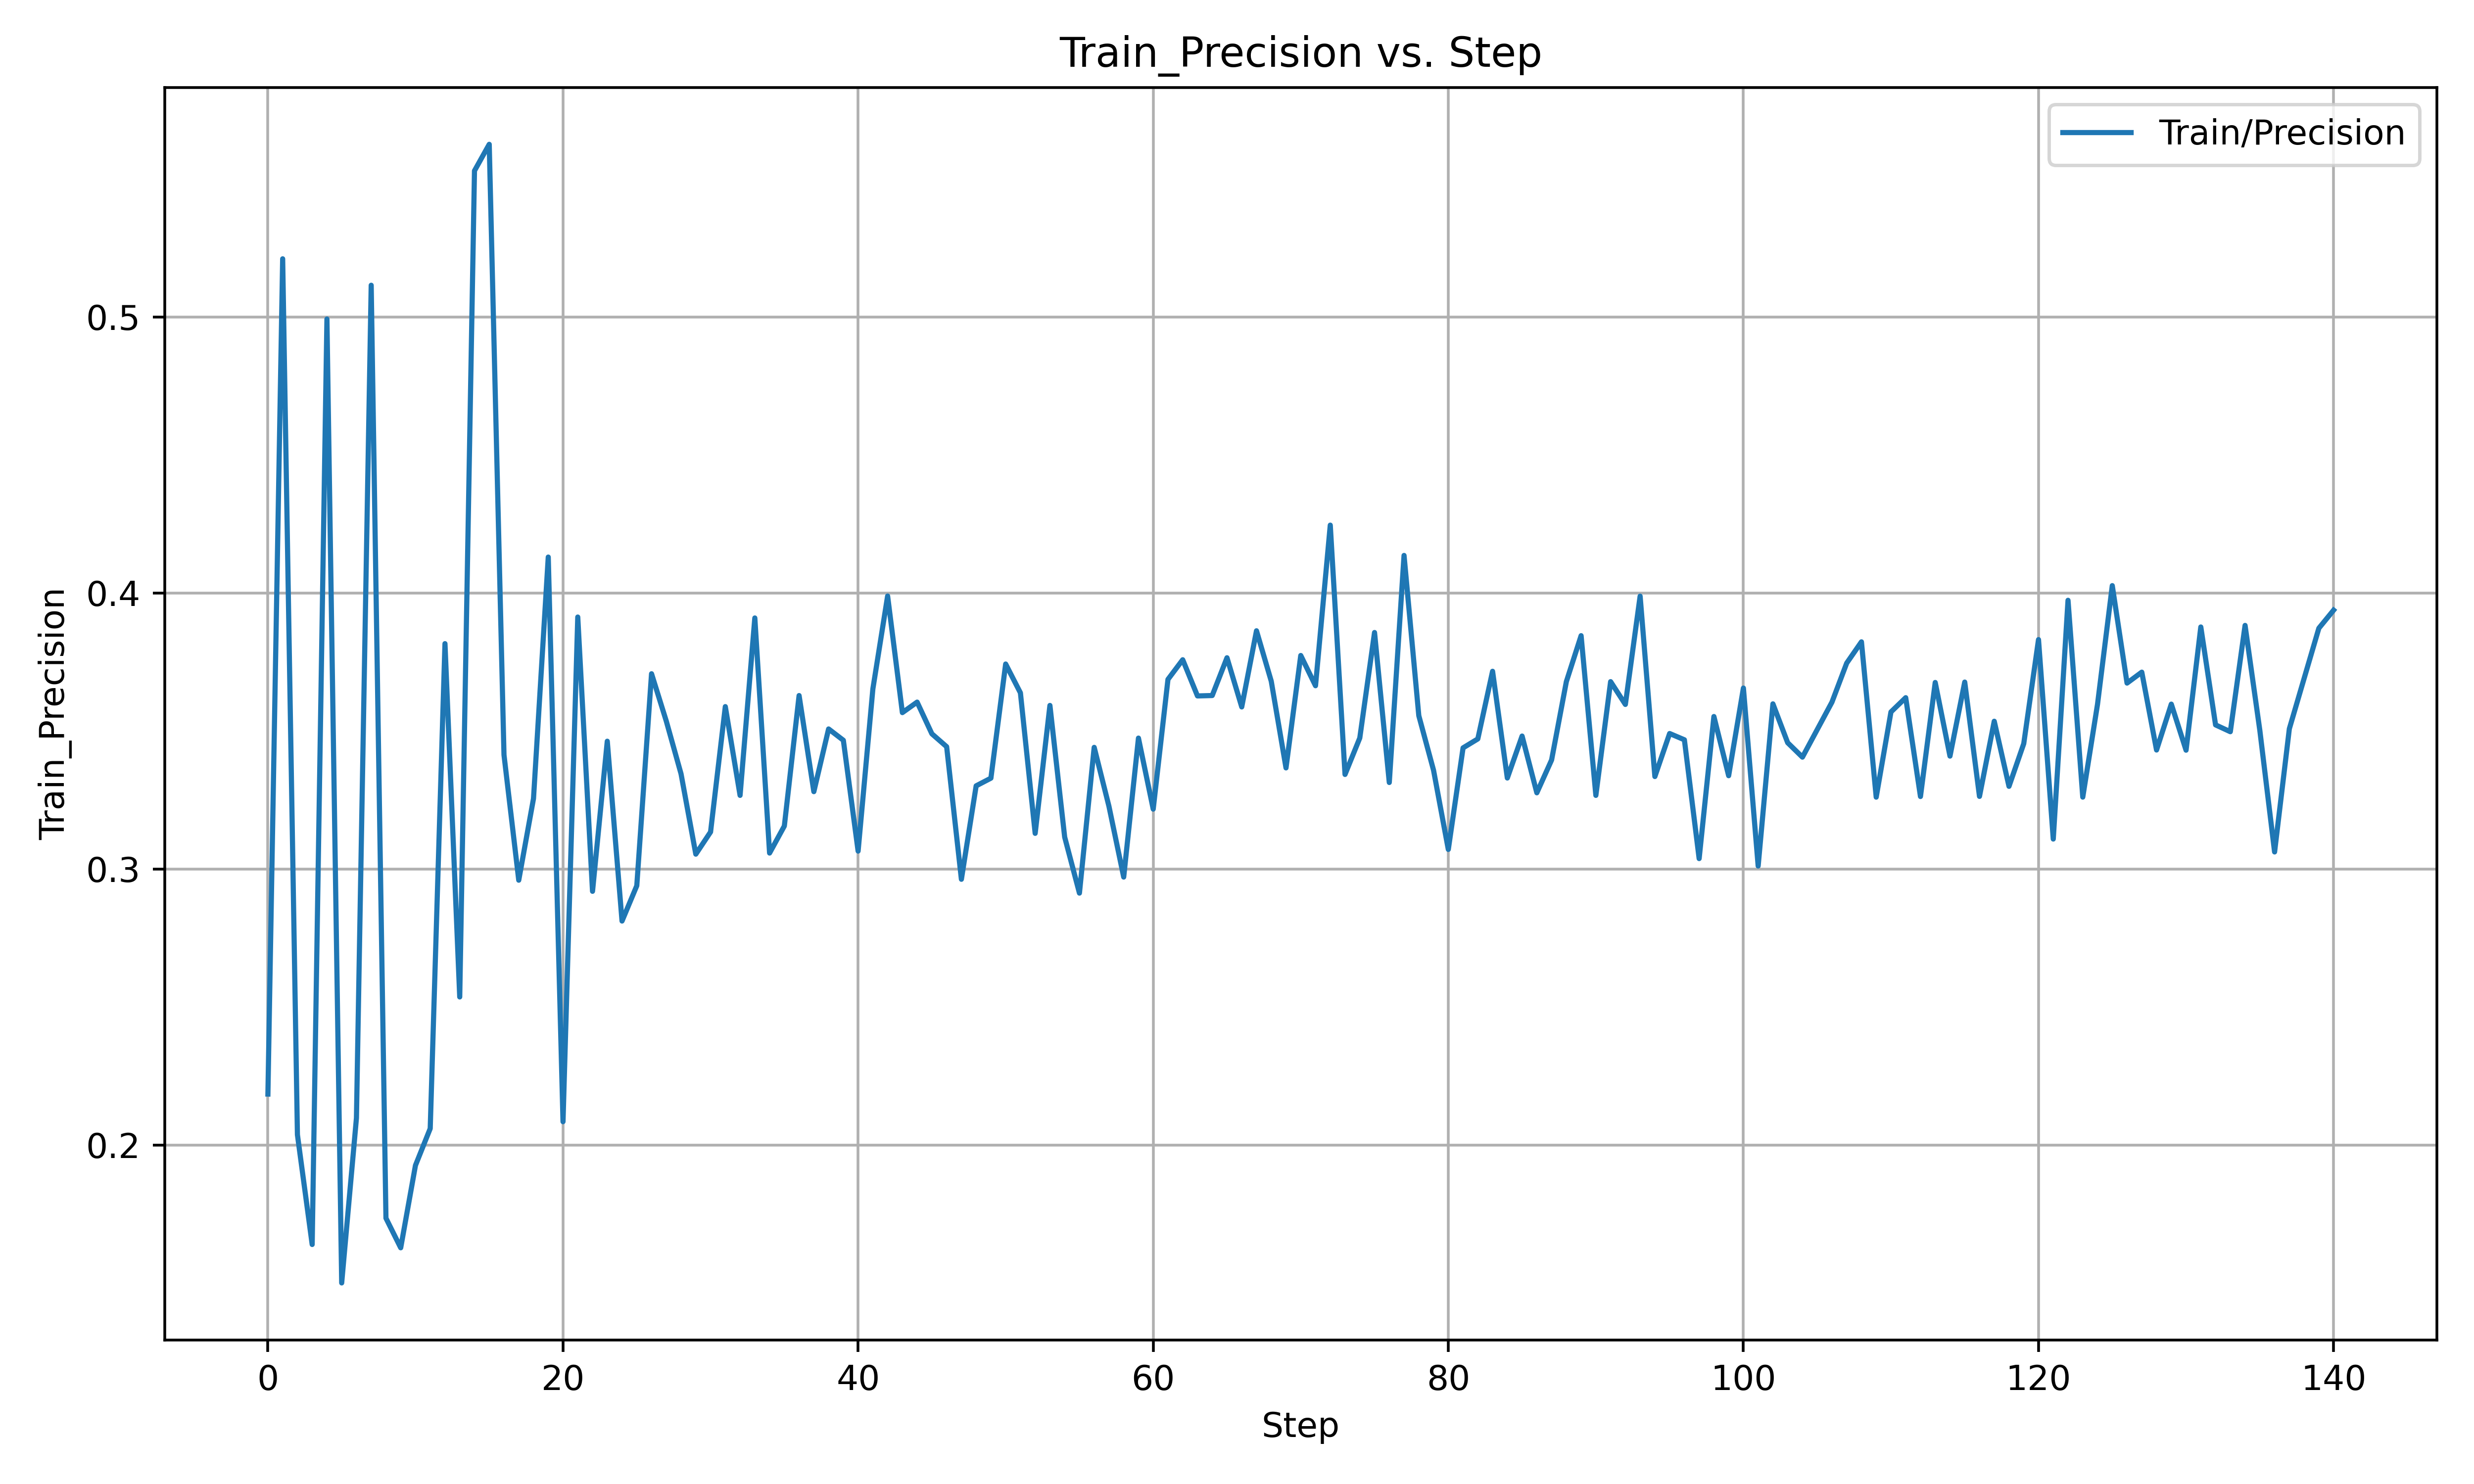
\includegraphics[width=\linewidth]{Train_Precision.png}
		\caption{Precision Curve}
	\end{subfigure}
	\hfill
	\begin{subfigure}[b]{0.32\textwidth}
		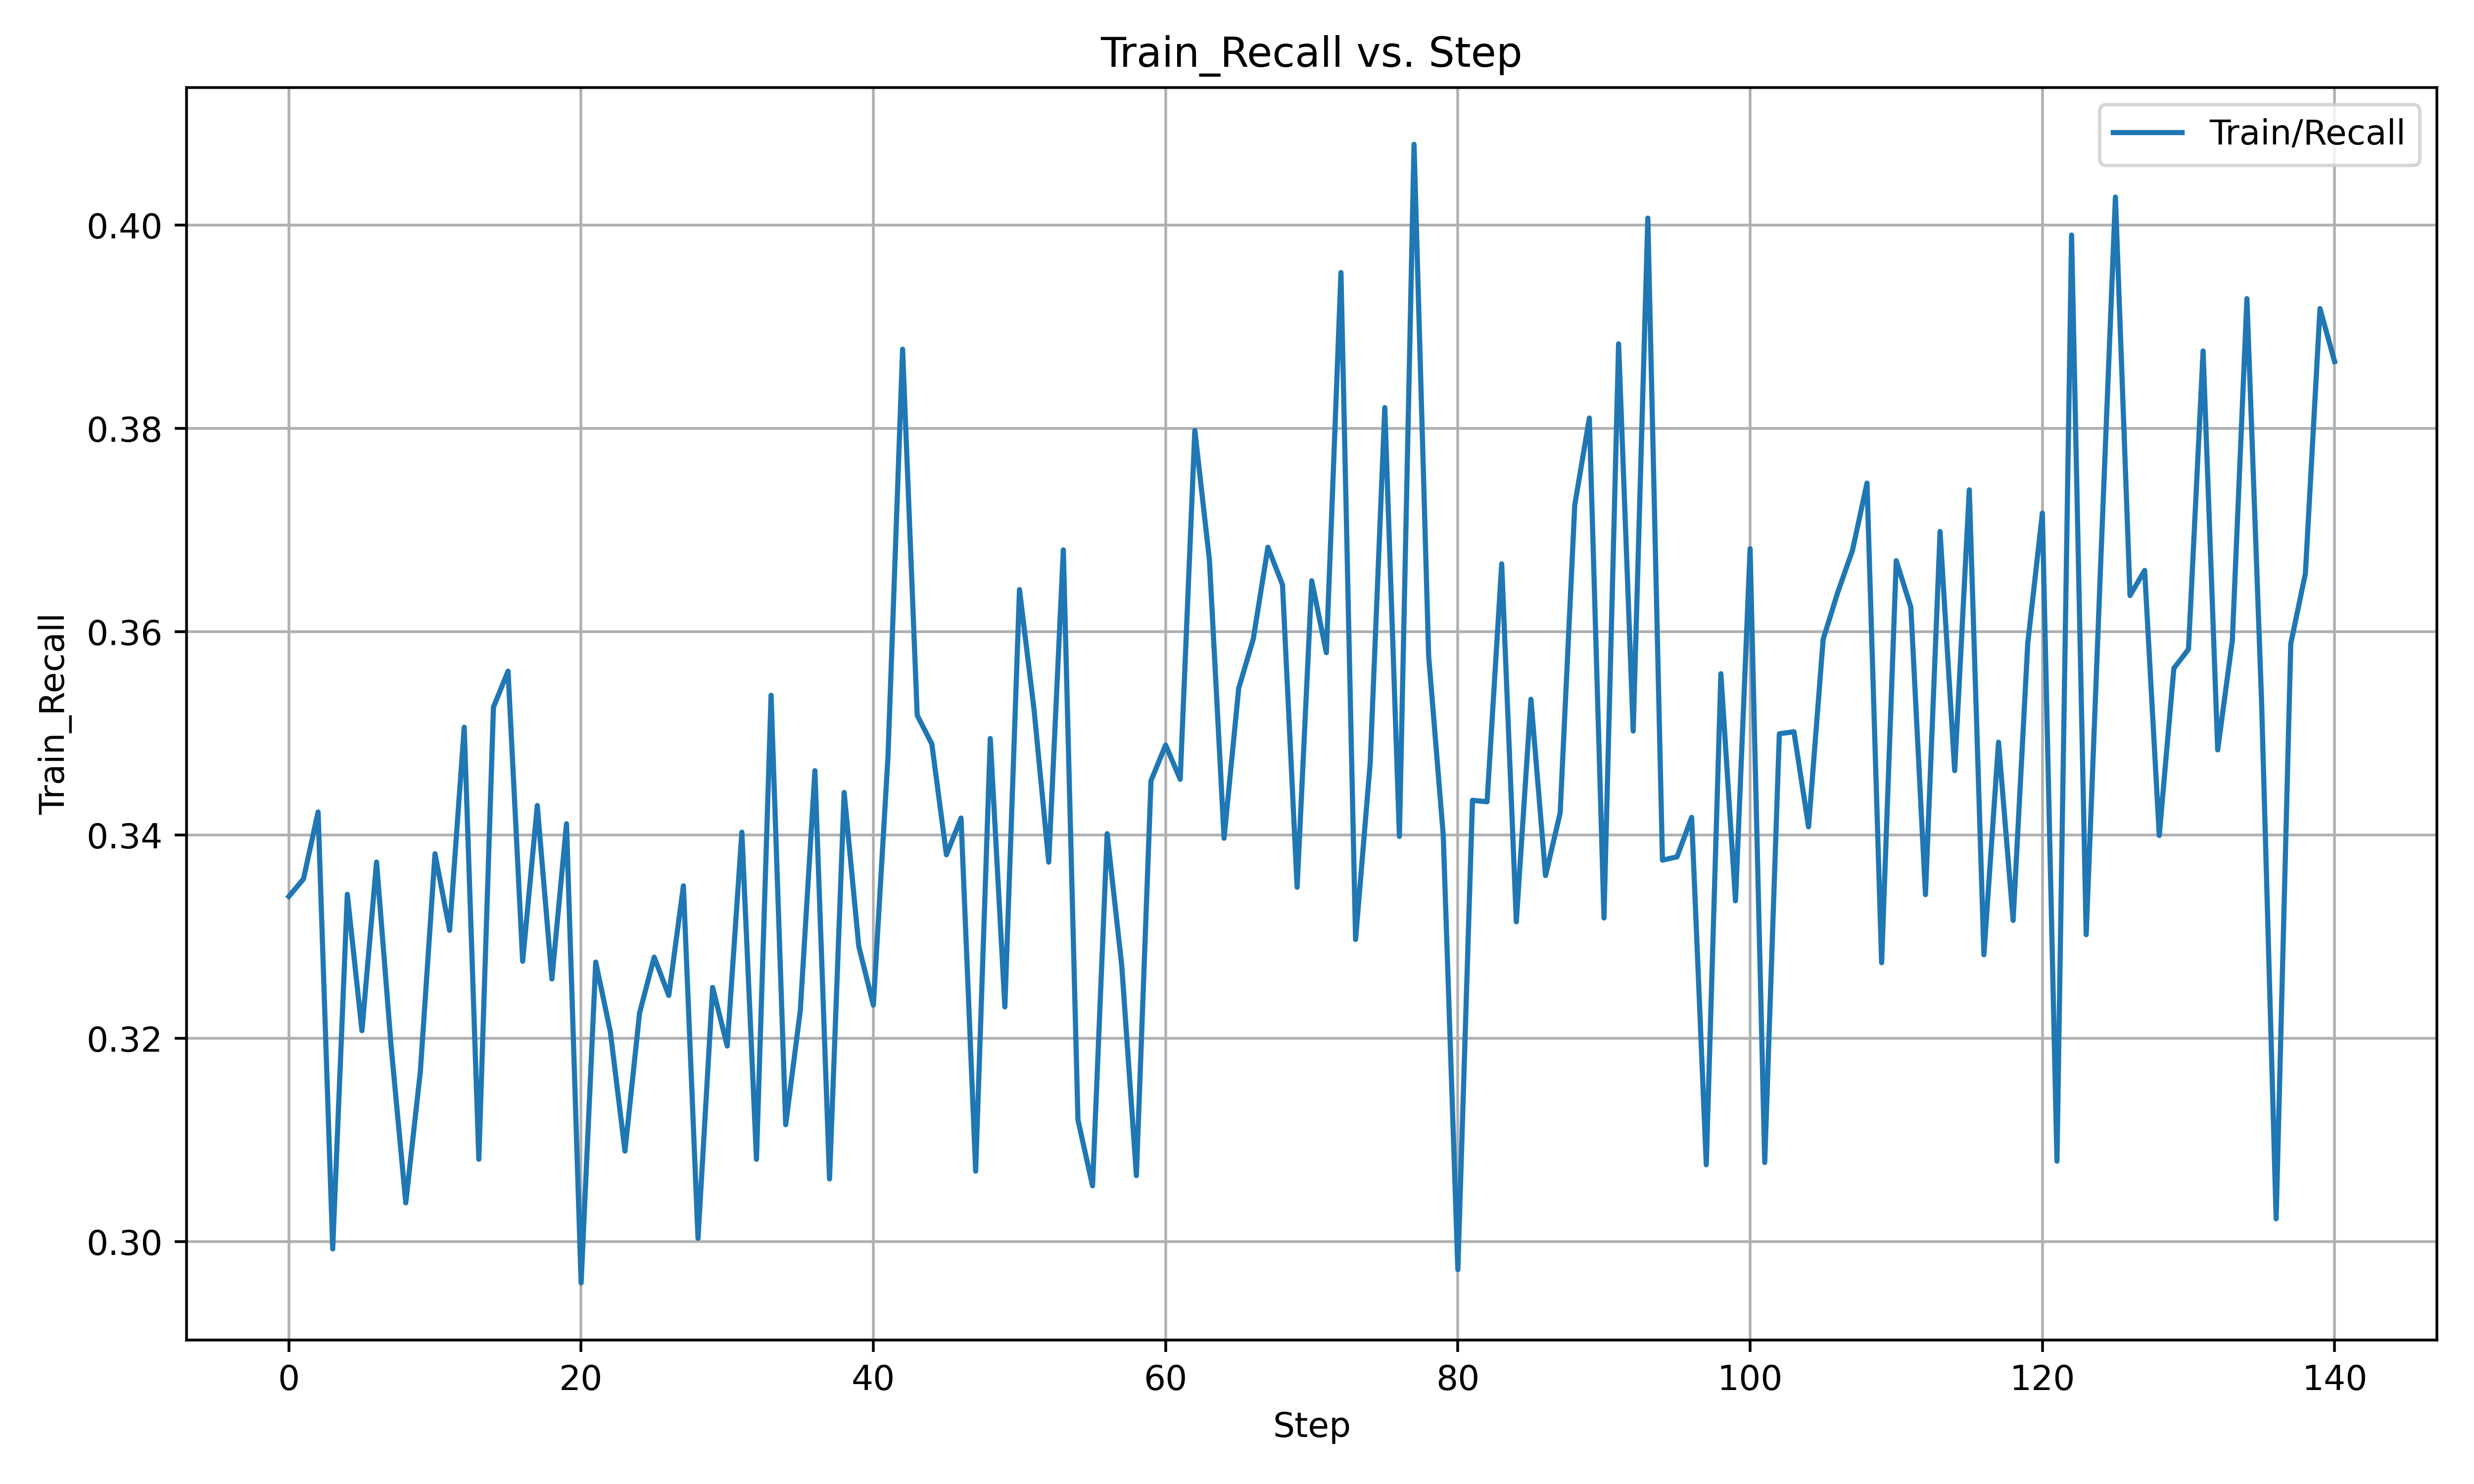
\includegraphics[width=\linewidth]{Train_Recall.png}
		\caption{Recall Curve}
	\end{subfigure}
	\caption{BERT model training performance.}
	\label{fig:bert_training_performance}
\end{figure}

Although BERT ultimately achieves our goal of improving Chinese financial sentiment classification, the presence of "meaningless" tokens in word clouds suggests that the model may struggle with specialized financial terminology. Furthermore, the low accuracy and F1 score indicate that the model may not be well-suited or well tune for the financial sentiment analysis task. Future work will focus on refining translation techniques, exploring Bayesian or traditional machine learning methods, and enhancing data filtering mechanisms to improve classification accuracy and interpretability.

%----------------------------------------
% 5. DISCUSSION
%----------------------------------------
\section{Discussion}
\label{sec:discussion}

Our multi-stage pipeline leverages translation to alleviate data scarcity, yet the performance and interpretability challenges remain. “Meaningless” tokens in word clouds reflect inadequate mapping of specialized English financial phrases into Chinese. Potential remedies include domain-specific dictionaries and graph-based methods that unify semantic representations across languages.

\paragraph{BERT vs. Bayesian Methods}
While BERT excels at capturing subtle sentiment cues, Bayesian and other classic machine learning models (e.g., random forests, SVM) can outperform deep neural networks, particularly when data are limited or transparency is critical. Bayesian frameworks, for example, provide posterior probabilities that quantify uncertainty, enhancing the trustworthiness of modeling outcomes in high-stakes environments like finance.

\paragraph{Alternative Approaches and Future Outlook}
We also foresee the growing importance of knowledge graphs or ontology-based approaches to better unify semantic representations, particularly when bridging linguistic gaps between English and Chinese. Future work will address these limitations by refining translation modules, exploring multi-lingual pre-training strategies, and examining simpler but interpretable classification algorithms.

%----------------------------------------
% 6. CONCLUSION AND FUTURE WORK
%----------------------------------------
\section{Conclusion and Future Work}
\label{sec:conclusion}

This paper proposed a comprehensive solution to Chinese financial sentiment analysis, underscoring the value of translation-based data augmentation, lexicon-assisted labeling, and BERT fine-tuning. Our empirical investigations confirm that the workflow substantially improves classification metrics compared to purely lexicon-based or simpler machine learning baselines. Nonetheless, translation quality shortfalls, noisy lexicon coverage, and interpretability gaps suggest the need for continued innovation:

\begin{itemize}
    \item \textbf{Refined Translation Techniques:} Incorporating domain-specific glossaries or graph-based representations may minimize semantic distortions.
    \item \textbf{Bayesian Interpretability:} Further exploration of Bayesian or conventional ML methods could yield comparable or superior performance while offering clearer insights into model uncertainty.
    \item \textbf{Advanced Data Filtering:} Enhanced mechanisms for filtering, verifying, and curating translated texts will boost final classification accuracy.
    \item \textbf{Expanded Modalities:} Future research might integrate other data sources (e.g., images, audio from earnings calls, or social media metrics) into a multi-modal sentiment model.
\end{itemize}

By addressing these fronts, we aim to develop robust automated sentiment systems that not only detect subtle emotional signals but also support transparent, accountable decision-making for financial market participants.

%----------------------------------------
% ACKNOWLEDGEMENTS
%----------------------------------------

\section*{Acknowledgements: Contribution of Authors}
The authors extend their profound gratitude to the instructors for their invaluable guidance and unwavering support throughout the duration of the course. Furthermore, they express sincere appreciation for the constructive feedback provided by their peers and the intellectually stimulating discussions that have significantly deepened their comprehension of the subject matter. In the course of this project, all members contributed equally to its completion. Specifically, Chuan Jia undertook the responsibility of drafting the report/paper, Bo Li contributed by providing the conceptual inspiration for the topic and delivering the presentation, while Sheng Su was responsible for the implementation of the code, as well as the revision and refinement of the report/paper. Notably, no group leader was designated for this project, as all members collaborated on an equal footing.

\section*{Acknowledgements: Observation}
The course itself is both vibrant and intellectually invigorating; however, the sheer breadth and density of the material prove overwhelming, leaving us thoroughly fatigued. While we have undoubtedly derived substantial intellectual enrichment from it, our diverse backgrounds and varying capacities have rendered it challenging to keep pace with the demands of the curriculum. We hold the utmost respect for the instructor's noble intentions and acknowledge the profound benefits we have reaped from this learning experience. Nevertheless, we humbly propose the possibility of dividing the content into at least two distinct courses in the future. Such an adjustment would enable students to assimilate the material more effectively and engage with the subject matter on a deeper level. We remain profoundly grateful for the privilege of participating in this course and are confident that the knowledge and skills acquired will serve as invaluable assets in our future endeavors.

\section*{Certification}
%----------------------------------------
% REFERENCES
%----------------------------------------
\bibliographystyle{unsrt}
\begin{thebibliography}{100}

\bibitem{ref1}
Vaswani, A.; Shazeer, N.; Parmar, N.; Uszkoreit, J.; Jones, L.; Gomez, A.~N.; Kaiser, {\L}.; Polosukhin, I. 
\newblock Attention is all you need.
\newblock {\em Advances in Neural Information Processing Systems}, 2017.

\bibitem{ref2}
Devlin, J.; Chang, M.~W.; Lee, K.; Toutanova, K.
\newblock BERT: Pre-training of Deep Bidirectional Transformers for Language Understanding.
\newblock In {\em Proceedings of the 2019 Conference of the North American Chapter of the Association for Computational Linguistics: Human Language Technologies (NAACL HLT)}, Minneapolis, MN, USA, 2--7 June 2019.

\bibitem{ref3}
Jiang, F.; Lee, J.~A.; Martin, X.; Zhou, G.
\newblock Manager sentiment and stock returns.
\newblock {\em Journal of Financial Economics}, \textbf{132}(1):126--149, 2019.

\bibitem{ref4}
Jiang, F.; Meng, L.; Tang, G.
\newblock Prediction of Stock Returns Using Media Text Sentiment.
\newblock {\em Economics Quarterly}, \textbf{20}(4):1323--1344, 2021.

\end{thebibliography}

\end{document}
